% Generated by Sphinx.
\def\sphinxdocclass{report}
\documentclass[letterpaper,10pt,spanish]{sphinxmanual}
\usepackage[utf8]{inputenc}
\DeclareUnicodeCharacter{00A0}{\nobreakspace}
\usepackage{cmap}
\usepackage[T1]{fontenc}
\usepackage{babel}
\usepackage{times}
\usepackage[Sonny]{fncychap}
\usepackage{longtable}
\usepackage{sphinx}
\usepackage{multirow}


\addto\captionsspanish{\renewcommand{\figurename}{Figura }}
\addto\captionsspanish{\renewcommand{\tablename}{Tabla }}
\floatname{literal-block}{Lista }



\title{libertya-doc Documentation}
\date{05 de February de 2016}
\release{1.0}
\author{Cooperativa Geneos Ltda.}
\newcommand{\sphinxlogo}{}
\renewcommand{\releasename}{Publicación}
\makeindex

\makeatletter
\def\PYG@reset{\let\PYG@it=\relax \let\PYG@bf=\relax%
    \let\PYG@ul=\relax \let\PYG@tc=\relax%
    \let\PYG@bc=\relax \let\PYG@ff=\relax}
\def\PYG@tok#1{\csname PYG@tok@#1\endcsname}
\def\PYG@toks#1+{\ifx\relax#1\empty\else%
    \PYG@tok{#1}\expandafter\PYG@toks\fi}
\def\PYG@do#1{\PYG@bc{\PYG@tc{\PYG@ul{%
    \PYG@it{\PYG@bf{\PYG@ff{#1}}}}}}}
\def\PYG#1#2{\PYG@reset\PYG@toks#1+\relax+\PYG@do{#2}}

\expandafter\def\csname PYG@tok@gd\endcsname{\def\PYG@tc##1{\textcolor[rgb]{0.63,0.00,0.00}{##1}}}
\expandafter\def\csname PYG@tok@gu\endcsname{\let\PYG@bf=\textbf\def\PYG@tc##1{\textcolor[rgb]{0.50,0.00,0.50}{##1}}}
\expandafter\def\csname PYG@tok@gt\endcsname{\def\PYG@tc##1{\textcolor[rgb]{0.00,0.27,0.87}{##1}}}
\expandafter\def\csname PYG@tok@gs\endcsname{\let\PYG@bf=\textbf}
\expandafter\def\csname PYG@tok@gr\endcsname{\def\PYG@tc##1{\textcolor[rgb]{1.00,0.00,0.00}{##1}}}
\expandafter\def\csname PYG@tok@cm\endcsname{\let\PYG@it=\textit\def\PYG@tc##1{\textcolor[rgb]{0.25,0.50,0.56}{##1}}}
\expandafter\def\csname PYG@tok@vg\endcsname{\def\PYG@tc##1{\textcolor[rgb]{0.73,0.38,0.84}{##1}}}
\expandafter\def\csname PYG@tok@m\endcsname{\def\PYG@tc##1{\textcolor[rgb]{0.13,0.50,0.31}{##1}}}
\expandafter\def\csname PYG@tok@mh\endcsname{\def\PYG@tc##1{\textcolor[rgb]{0.13,0.50,0.31}{##1}}}
\expandafter\def\csname PYG@tok@cs\endcsname{\def\PYG@tc##1{\textcolor[rgb]{0.25,0.50,0.56}{##1}}\def\PYG@bc##1{\setlength{\fboxsep}{0pt}\colorbox[rgb]{1.00,0.94,0.94}{\strut ##1}}}
\expandafter\def\csname PYG@tok@ge\endcsname{\let\PYG@it=\textit}
\expandafter\def\csname PYG@tok@vc\endcsname{\def\PYG@tc##1{\textcolor[rgb]{0.73,0.38,0.84}{##1}}}
\expandafter\def\csname PYG@tok@il\endcsname{\def\PYG@tc##1{\textcolor[rgb]{0.13,0.50,0.31}{##1}}}
\expandafter\def\csname PYG@tok@go\endcsname{\def\PYG@tc##1{\textcolor[rgb]{0.20,0.20,0.20}{##1}}}
\expandafter\def\csname PYG@tok@cp\endcsname{\def\PYG@tc##1{\textcolor[rgb]{0.00,0.44,0.13}{##1}}}
\expandafter\def\csname PYG@tok@gi\endcsname{\def\PYG@tc##1{\textcolor[rgb]{0.00,0.63,0.00}{##1}}}
\expandafter\def\csname PYG@tok@gh\endcsname{\let\PYG@bf=\textbf\def\PYG@tc##1{\textcolor[rgb]{0.00,0.00,0.50}{##1}}}
\expandafter\def\csname PYG@tok@ni\endcsname{\let\PYG@bf=\textbf\def\PYG@tc##1{\textcolor[rgb]{0.84,0.33,0.22}{##1}}}
\expandafter\def\csname PYG@tok@nl\endcsname{\let\PYG@bf=\textbf\def\PYG@tc##1{\textcolor[rgb]{0.00,0.13,0.44}{##1}}}
\expandafter\def\csname PYG@tok@nn\endcsname{\let\PYG@bf=\textbf\def\PYG@tc##1{\textcolor[rgb]{0.05,0.52,0.71}{##1}}}
\expandafter\def\csname PYG@tok@no\endcsname{\def\PYG@tc##1{\textcolor[rgb]{0.38,0.68,0.84}{##1}}}
\expandafter\def\csname PYG@tok@na\endcsname{\def\PYG@tc##1{\textcolor[rgb]{0.25,0.44,0.63}{##1}}}
\expandafter\def\csname PYG@tok@nb\endcsname{\def\PYG@tc##1{\textcolor[rgb]{0.00,0.44,0.13}{##1}}}
\expandafter\def\csname PYG@tok@nc\endcsname{\let\PYG@bf=\textbf\def\PYG@tc##1{\textcolor[rgb]{0.05,0.52,0.71}{##1}}}
\expandafter\def\csname PYG@tok@nd\endcsname{\let\PYG@bf=\textbf\def\PYG@tc##1{\textcolor[rgb]{0.33,0.33,0.33}{##1}}}
\expandafter\def\csname PYG@tok@ne\endcsname{\def\PYG@tc##1{\textcolor[rgb]{0.00,0.44,0.13}{##1}}}
\expandafter\def\csname PYG@tok@nf\endcsname{\def\PYG@tc##1{\textcolor[rgb]{0.02,0.16,0.49}{##1}}}
\expandafter\def\csname PYG@tok@si\endcsname{\let\PYG@it=\textit\def\PYG@tc##1{\textcolor[rgb]{0.44,0.63,0.82}{##1}}}
\expandafter\def\csname PYG@tok@s2\endcsname{\def\PYG@tc##1{\textcolor[rgb]{0.25,0.44,0.63}{##1}}}
\expandafter\def\csname PYG@tok@vi\endcsname{\def\PYG@tc##1{\textcolor[rgb]{0.73,0.38,0.84}{##1}}}
\expandafter\def\csname PYG@tok@nt\endcsname{\let\PYG@bf=\textbf\def\PYG@tc##1{\textcolor[rgb]{0.02,0.16,0.45}{##1}}}
\expandafter\def\csname PYG@tok@nv\endcsname{\def\PYG@tc##1{\textcolor[rgb]{0.73,0.38,0.84}{##1}}}
\expandafter\def\csname PYG@tok@s1\endcsname{\def\PYG@tc##1{\textcolor[rgb]{0.25,0.44,0.63}{##1}}}
\expandafter\def\csname PYG@tok@gp\endcsname{\let\PYG@bf=\textbf\def\PYG@tc##1{\textcolor[rgb]{0.78,0.36,0.04}{##1}}}
\expandafter\def\csname PYG@tok@sh\endcsname{\def\PYG@tc##1{\textcolor[rgb]{0.25,0.44,0.63}{##1}}}
\expandafter\def\csname PYG@tok@ow\endcsname{\let\PYG@bf=\textbf\def\PYG@tc##1{\textcolor[rgb]{0.00,0.44,0.13}{##1}}}
\expandafter\def\csname PYG@tok@sx\endcsname{\def\PYG@tc##1{\textcolor[rgb]{0.78,0.36,0.04}{##1}}}
\expandafter\def\csname PYG@tok@bp\endcsname{\def\PYG@tc##1{\textcolor[rgb]{0.00,0.44,0.13}{##1}}}
\expandafter\def\csname PYG@tok@c1\endcsname{\let\PYG@it=\textit\def\PYG@tc##1{\textcolor[rgb]{0.25,0.50,0.56}{##1}}}
\expandafter\def\csname PYG@tok@kc\endcsname{\let\PYG@bf=\textbf\def\PYG@tc##1{\textcolor[rgb]{0.00,0.44,0.13}{##1}}}
\expandafter\def\csname PYG@tok@c\endcsname{\let\PYG@it=\textit\def\PYG@tc##1{\textcolor[rgb]{0.25,0.50,0.56}{##1}}}
\expandafter\def\csname PYG@tok@mf\endcsname{\def\PYG@tc##1{\textcolor[rgb]{0.13,0.50,0.31}{##1}}}
\expandafter\def\csname PYG@tok@err\endcsname{\def\PYG@bc##1{\setlength{\fboxsep}{0pt}\fcolorbox[rgb]{1.00,0.00,0.00}{1,1,1}{\strut ##1}}}
\expandafter\def\csname PYG@tok@kd\endcsname{\let\PYG@bf=\textbf\def\PYG@tc##1{\textcolor[rgb]{0.00,0.44,0.13}{##1}}}
\expandafter\def\csname PYG@tok@ss\endcsname{\def\PYG@tc##1{\textcolor[rgb]{0.32,0.47,0.09}{##1}}}
\expandafter\def\csname PYG@tok@sr\endcsname{\def\PYG@tc##1{\textcolor[rgb]{0.14,0.33,0.53}{##1}}}
\expandafter\def\csname PYG@tok@mo\endcsname{\def\PYG@tc##1{\textcolor[rgb]{0.13,0.50,0.31}{##1}}}
\expandafter\def\csname PYG@tok@mi\endcsname{\def\PYG@tc##1{\textcolor[rgb]{0.13,0.50,0.31}{##1}}}
\expandafter\def\csname PYG@tok@kn\endcsname{\let\PYG@bf=\textbf\def\PYG@tc##1{\textcolor[rgb]{0.00,0.44,0.13}{##1}}}
\expandafter\def\csname PYG@tok@o\endcsname{\def\PYG@tc##1{\textcolor[rgb]{0.40,0.40,0.40}{##1}}}
\expandafter\def\csname PYG@tok@kr\endcsname{\let\PYG@bf=\textbf\def\PYG@tc##1{\textcolor[rgb]{0.00,0.44,0.13}{##1}}}
\expandafter\def\csname PYG@tok@s\endcsname{\def\PYG@tc##1{\textcolor[rgb]{0.25,0.44,0.63}{##1}}}
\expandafter\def\csname PYG@tok@kp\endcsname{\def\PYG@tc##1{\textcolor[rgb]{0.00,0.44,0.13}{##1}}}
\expandafter\def\csname PYG@tok@w\endcsname{\def\PYG@tc##1{\textcolor[rgb]{0.73,0.73,0.73}{##1}}}
\expandafter\def\csname PYG@tok@kt\endcsname{\def\PYG@tc##1{\textcolor[rgb]{0.56,0.13,0.00}{##1}}}
\expandafter\def\csname PYG@tok@sc\endcsname{\def\PYG@tc##1{\textcolor[rgb]{0.25,0.44,0.63}{##1}}}
\expandafter\def\csname PYG@tok@sb\endcsname{\def\PYG@tc##1{\textcolor[rgb]{0.25,0.44,0.63}{##1}}}
\expandafter\def\csname PYG@tok@k\endcsname{\let\PYG@bf=\textbf\def\PYG@tc##1{\textcolor[rgb]{0.00,0.44,0.13}{##1}}}
\expandafter\def\csname PYG@tok@se\endcsname{\let\PYG@bf=\textbf\def\PYG@tc##1{\textcolor[rgb]{0.25,0.44,0.63}{##1}}}
\expandafter\def\csname PYG@tok@sd\endcsname{\let\PYG@it=\textit\def\PYG@tc##1{\textcolor[rgb]{0.25,0.44,0.63}{##1}}}

\def\PYGZbs{\char`\\}
\def\PYGZus{\char`\_}
\def\PYGZob{\char`\{}
\def\PYGZcb{\char`\}}
\def\PYGZca{\char`\^}
\def\PYGZam{\char`\&}
\def\PYGZlt{\char`\<}
\def\PYGZgt{\char`\>}
\def\PYGZsh{\char`\#}
\def\PYGZpc{\char`\%}
\def\PYGZdl{\char`\$}
\def\PYGZhy{\char`\-}
\def\PYGZsq{\char`\'}
\def\PYGZdq{\char`\"}
\def\PYGZti{\char`\~}
% for compatibility with earlier versions
\def\PYGZat{@}
\def\PYGZlb{[}
\def\PYGZrb{]}
\makeatother

\renewcommand\PYGZsq{\textquotesingle}

\begin{document}
\shorthandoff{"}
\maketitle
\tableofcontents
\phantomsection\label{index::doc}


Índice de contenidos:


\chapter{Acerca de Libertya Doc}
\label{all-about-me:acerca-de-libertya-doc}\label{all-about-me::doc}\label{all-about-me:documentacion-de-libertya-erp-mrp}

\section{Libertya ERP}
\label{all-about-me:libertya-erp}
Libertya es un poderoso ERP con toda su funcionalidad desarrollada y distribuida como software libre; está basado en tecnología multiplataforma, y es completamente personalizable y adaptable a las necesidades de cualquier empresa. Su arquitectura y componentes son totalmente escalables. Además, está diseñado para ser integrado fácilmente con cualquier ecosistema de software pre-existente.

\textbf{Beneficios que diferencian a Libertya}
\begin{itemize}
\item {} 
La empresa usuaria posee un completo control de su implementación sin estar obligada a convenios de mantenimiento obligatorios.

\item {} 
El código del producto y toda su documentación asociada están disponibles desde un primer momento.

\item {} 
Independencia total del proveedor y acceso permanente de una numerosa y dinámica comunidad de usuarios.

\item {} 
Capacitación integral y asesoramiento profesional incluyendo - en caso de ser de interés - el diseño de su arquitectura interna y detalles constructivos del producto.

\item {} 
Componentes y aplicaciones complementarias especialmente diseñadas para extender e integrar Libertya a otros productos de software.

\end{itemize}

\textbf{Licencia}

Libertya ERP es un Software de Gestión Libre regulado por la licencia LPLB 1.0 (Licencia Pública Libertya versión 1.0) mediante la cual el producto puede ser utilizado sin costo de licencias con el 100\% de la funcionalidad disponible.

\textbf{Código abierto}

Código abierto (del inglés open source) es el término con el que se conoce al software distribuido y desarrollado libremente. Fue utilizado por primera vez en 1998 por algunos usuarios de la comunidad del software libre, tratando de usarlo como reemplazo al ambiguo nombre original en inglés del software libre (free software).


\section{Proyecto de Documentación}
\label{all-about-me:proyecto-de-documentacion}
Este proyecto busca dotar al sistema, de un paquete de documentación completa. Esta documentación, busca desarrollarse de manera colaborativa.

\textbf{Como Colaborar}


\section{Colaboradores}
\label{all-about-me:colaboradores}

\subsection{Acerca de Geneos}
\label{all-about-geneos:acerca-de-geneos}\label{all-about-geneos::doc}
\textbf{Somos}
\begin{quote}

Una cooperativa conformada por profesionales de la informática, las comunicaciones y el diseño, lo que nos permite trabajar de manera integral en la búsqueda de innovación, la mejora continua y la calidad. Nos dedicamos a implementar proyectos de tecnología, basados en Software Libre, que contribuyan a mejorar y potenciar el modelo de negocios de nuestros clientes.

Ofrecemos nuestra experiencia de más de 15 años desarrollando software para encontrar las mejores soluciones posibles. Contamos además con diversas experiencias en metodología ágiles para la mejora continua, normas y procedimientos, seguridad de la información, posicionamiento en buscadores,presencia digital, publicidad, comunicación y diseño gráfico.
\end{quote}

\textbf{una cooperativa de trabajo}
\begin{quote}

Entendemos el cooperativismo como la forma de resignificar el trabajo y construir nuevas formas de organización en torno a este. Creemos en el cooperativismo como  un herramienta de transformación, que permite lograr una manera democrática y participativa de gestionar las formas y objetivos del trabajo de las personas.
\end{quote}

\textbf{de Tecnología, Innovación y Conocimiento}
\begin{quote}

Nos dedicamos a brindar soluciones informáticas a otras organizaciones, empresas o personas. El trabajo que realizamos consiste en el desarrollo de software, es decir, la creación de sistemas que posibilitan la resolución de una problemática específica. Las cooperativas TICs se dedican al diseño de estas aplicaciones y a garantizar su correcta implementación. Por otro lado, ofrecemos servicio de consultoría o soporte técnico y auditorías sobre los sistemas que una organización ya posee. Otro de los servicios ofrecidos son las capacitaciones a las empresas en el uso de los sistemas.
\end{quote}

\textbf{basados en Software Libre}
\begin{quote}

El software libre fomenta el trabajo colaborativo mediante comunidades de desarrollo, tiene potencial para dar soluciones y respuestas a todo tipo de requerimientos y no necesita licencias para su uso y desarrollo. Además, posee
estándares abiertos y garantiza la seguridad.
\end{quote}

{\hfill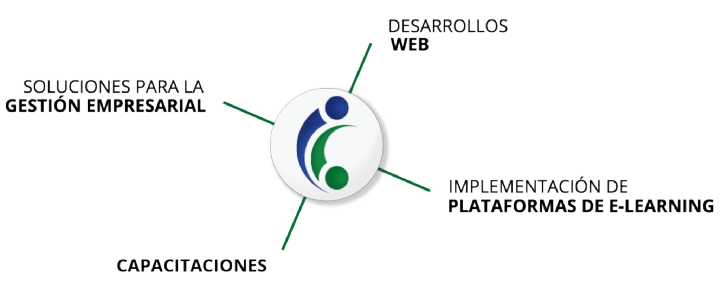
\includegraphics{coop_servicios.png}\hfill}


\chapter{Documentación técnica de Libertya}
\label{tecnica::doc}\label{tecnica:documentacion-tecnica-de-libertya}

\section{Introducción}
\label{tecnica:introduccion}
\textbf{Consideraciones}
\begin{itemize}
\item {} 
La presente guía, es desarrollada en el contecto de la instalación de LIbertya ERP sobre la distribución de Linux \textbf{Ubuntu}, en otras distribuciones, algunas partes de la guía, pueden requerir alternativas que no serán abordadas.

\end{itemize}

\textbf{Pasos}
\begin{enumerate}
\item {} 
Instalación de Java

\item {} 
Instalación de Postgres SQL

\item {} 
Creación de base de datos para Libertya

\item {} 
Instalación de Libertya

\item {} 
Configuración de backups automáticos.

\item {} 
Instalación de Eclipse

\item {} 
Descarga de código de Libertya.

\item {} 
Configuración de Eclipse.

\end{enumerate}


\section{Instalación de Java}
\label{tecnica:instalacion-de-java}

\section{Instalación de Postgres SQL}
\label{tecnica:instalacion-de-postgres-sql}

\section{Creación de base de datos para Libertya}
\label{tecnica:creacion-de-base-de-datos-para-libertya}

\section{Instalación de Libertya}
\label{tecnica:instalacion-de-libertya}

\section{Configuración de backups automáticos}
\label{tecnica:configuracion-de-backups-automaticos}

\section{Instalación de Eclipse}
\label{tecnica:instalacion-de-eclipse}

\section{Descarga de código de Libertya}
\label{tecnica:descarga-de-codigo-de-libertya}

\section{Configuración y ejecusión de Libertya en Eclipse}
\label{tecnica:configuracion-y-ejecusion-de-libertya-en-eclipse}

\section{Configuración y debug de Libertya en Eclipse}
\label{tecnica:configuracion-y-debug-de-libertya-en-eclipse}

\chapter{Primeros Pasos}
\label{acceso:primeros-pasos}\label{acceso::doc}

\section{Acceso}
\label{acceso:acceso}
En la ventana de \textbf{Entrada al Sistema}, en la pestaña \textbf{Conexión}, se debe completar:
\begin{enumerate}
\item {} 
\textbf{Servidor:} Esta dato ya está configurado por el administrador del sistema y no debe ser modificado por el usuario.

\item {} 
\textbf{Usuario:} ingrese su usuario de acceso al sistema. Tenga en cuenta que el sistema es key sensitive, es decir, discrimina mayúsculas y minúsculas en el tipeo. Así entonces, a modo de ejemplo: el usuario Juan no es el mismo que el usuario JUAN.

\item {} 
\textbf{Contraseña:} ingrese su usuario de acceso al sistema.

\item {} 
\textbf{Lenguaje:} Ud. debe seleccionar el lenguaje que corresponda. Para la localización Argentina, Español (Argentina).

\end{enumerate}
\begin{figure}[htbp]
\centering
\capstart

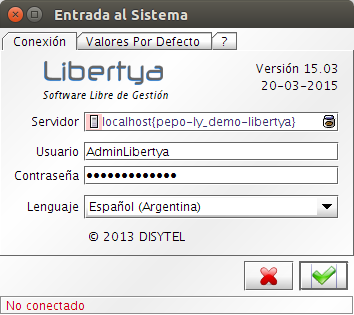
\includegraphics{ly_login.png}
\caption{Imagen 1: Ingreso al Sistema Pantalla 1}\end{figure}

Si Ud. tipea el Usuario y Contraseña correctamente, aparecerá en pantalla la pestaña Valores por Defecto (Imagen 2), donde se debe completar:
\begin{enumerate}
\item {} 
\textbf{Perfil:} El Sistema Libertya viene preconfigurado con cuatro perfiles (más un perfil de Administrador de la Compañía que define parámetros comunes a todos los demás usuarios), a los cuales se pueden agregar más en función de las necesidades de la organización. Elija uno de los perfiles.

\item {} 
\textbf{Compañía:} El Sistema Libertya viene preconfigurado con una compañía, a la cual se pueden agregar otras en función de las necesidades de la organización. Elija en este punto una de las compañías.

\item {} 
\textbf{Organización:} El Sistema Libertya viene preconfigurado con una organización, a la cual se pueden agregar otras en función de las necesidades de la estructura organizacional. Elija una de las organizaciones.

\item {} 
\textbf{Almacén:} El Sistema Libertya viene preconfigurado con un almacén, a la cual se pueden agregar otros en función de las necesidades de la estructura organizacional. Elija una de los almacenes. El almacén en algunos modelos de negocio se suele llamar Depósito, en otros salón de ventas, etc.

\item {} 
\textbf{Fecha:} El sistema Libertya toma del sistema operativo la fecha de trabajo, pero la misma puede ser modificada en este punto. En caso de ser necesario, haga un click con el mouse sobre el botón (31) que aparece sobre el costado derecho de la fecha que muestra el sistema, y seleccione la fecha que desea sobre la opción calendario. Tenga en cuenta que hacer esto implica que los movimientos se registrarán con la fecha que Ud. está indicando en este momento.

\item {} 
\textbf{Impresora:} El sistema Libertya le permite elegir la impresora de trabajo que se utilizará para imprimir los informes y listados del sistema. En este punto Ud. debe seleccionar la impresora que utilizará durante la sesión, pudiendo elegir entre todas las impresoras que Ud. tenga ya configuradas en su sistema operativo.

\end{enumerate}
\begin{figure}[htbp]
\centering
\capstart

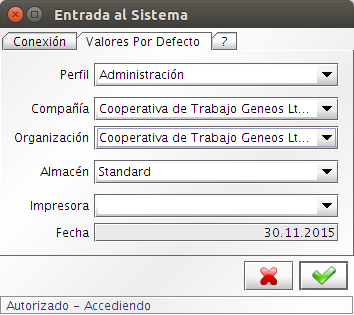
\includegraphics{ly_login_rol.png}
\caption{Imagen 2: Ingreso al Sistema Pantalla 2}\end{figure}


\chapter{Estructura de Aplicación}
\label{estructura:estructura-de-aplicacion}\label{estructura::doc}

\section{Pantalla principal}
\label{estructura:pantalla-principal}
Una vez validados los datos de acceso, el sistema presenta la ventana principal, como puede verse a continuación:
\begin{figure}[htbp]
\centering
\capstart

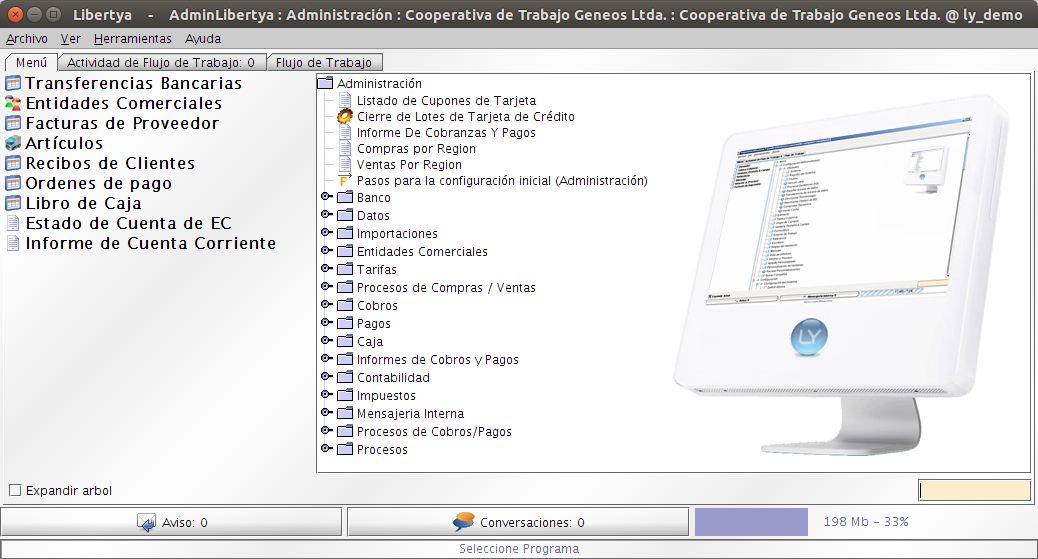
\includegraphics{ly_inicio.png}
\caption{Imagen 3: Pantalla Principal}\end{figure}


\section{Área de Trabajo}
\label{estructura:area-de-trabajo}
En el menú de la aplicación (área a la derecha) aparecen todos los componentes a los que se tiene acceso.

El menú se construye en modo árbol de forma que se pueden agrupar los componentes en carpetas. La configuración depende de los permisos que tenga el usuario y por lo tanto del rol con el que haya hecho login.

Existe dos manera de navegar a través del menú:
\begin{enumerate}
\item {} 
Haciendo doble click con el botón de mouse en las carpetas, y con un solo click para que se abra la ventana, procesos o informe a los que se quiera acceder.

\item {} 
La aplicación cuenta con una búsqueda sobre el menú, abajo a la derecha existe un campo de texto que nos permite ingresar el nombre de la utilidad que deseamos utilizar (Ventana, proceso o informe). Cuando se presiona la tecla Enter va a buscar la palabra ingresada, si existe mas de una palabra presionando de nuevo Enter salta a la siguiente opción. Una vez encontrada la funcionalidad con la tecla Ctrl + Enter se puede acceder a la funcionalidad.

\end{enumerate}


\section{Iconos del menú}
\label{estructura:iconos-del-menu}
En el árbol que forma el menú podemos encontrar cinco clases de iconos:
\begin{enumerate}
\item {} 
\textbf{Carpetas:} Cada carpeta contiene más elementos, ya sea ventanas de trabajo , procesos o informes. Cada carpeta contempla una temática del sistema, así es como podemos encontrar carpetas denominadas VENTAS, ALMACÉN, COMPRAS, etc. Para ver el contenido de una carpeta, haga click con el botón izquierdo del mouse sobre el botón que se encuentra justo a la izquierda de la carpeta a expandir.

\item {} 
\textbf{Ventanas:} Permite la introducción, consulta y modificación de datos, y desde ella se realizan la mayoría de actividades de interacción del usuario y la aplicación.

\item {} 
\textbf{Procesos:} Partiendo de los parámetros, datos o condiciones que asigne e introduzca el usuario, la aplicación realizara operaciones automáticas como la generación de albaranes o facturas, procesos de pedidos, etc.

\item {} 
\textbf{Informes:} Permite visualizar e imprimir la información de la aplicación según las condiciones definidas por el usuario. Por ejemplo permite visualizar los vencimientos, los últimos movimientos de stock, etc. Cualquier documento salida del sistema de gestión es factible de ser procesado como un informe.

\item {} 
\textbf{Flujo de trabajo:} Muestra una serie de actividades relacionadas entre si, que deben de irse completando en un orden dado, a fin de alimentar de datos de las actividades siguientes y obtener un resultado determinado. Ejemplos típicos son la configuración de artículos y entidades comerciales, o todos los sucesivos pasos de un proceso de negocio. Los flujos de trabajo se utilizaran, típicamente, por los usuarios encargados de la carga inicial de datos y mantenimiento de la aplicación con el fin de seguir un protocolo o procedimiento común en todos los casos que normalice un determinado proceso de negocio complejo.

\end{enumerate}

Adicionalmente, se dispone de la barra de acceso rápido situada a todo lo largo de la parte izquierda del menú. Para añadir ventanas o procesos a dicha barra, solo hay que hacer click con el botón derecho sobre el elemento para que se visualice la opción de Añadir a barra, y confirmar dicho mensaje con un click del botón izquierdo del ratón.


\section{Estructura de una ventana}
\label{estructura:estructura-de-una-ventana}
En algunas de las ventanas, debido a la alta cantidad de registros que contiene, aparecerá una ventana inicial de selección o de búsqueda similar a la que muestra la figura siguiente:
\begin{figure}[htbp]
\centering
\capstart

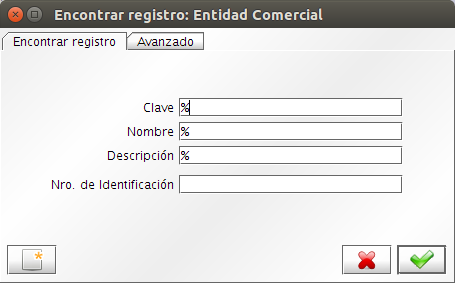
\includegraphics{ly_busqueda.png}
\caption{Imagen 4: Ventana de búsqueda de registros}\end{figure}

En función de los parámetros ingresados el sistema filtra los resultados que aparecen en una ventana con la siguiente estructura:
\begin{figure}[htbp]
\centering
\capstart

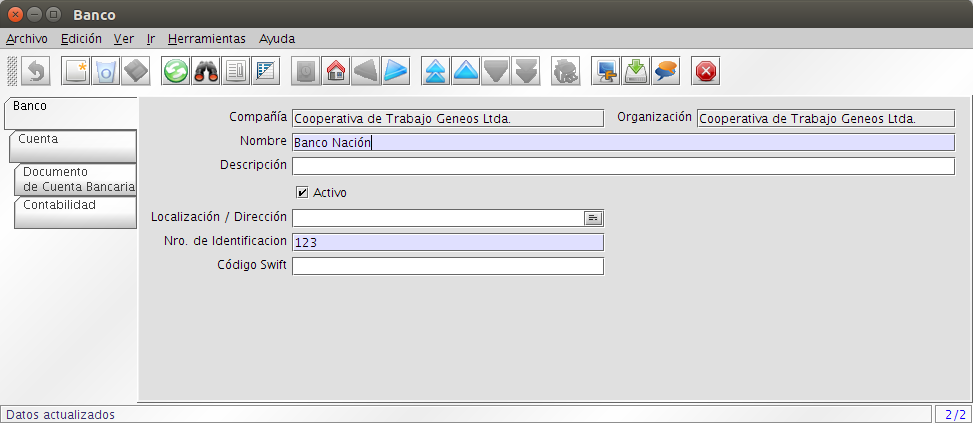
\includegraphics{ly_banco.png}
\caption{Imagen 5: Estructura de Ventanas}\end{figure}

Una ventana se organiza segmentando la información en Pestañas, para este caso como un banco puede tener varias cuentas tendremos esa relación representada en Pestañas anidadas, como puede verse a continuación:
\begin{figure}[htbp]
\centering
\capstart

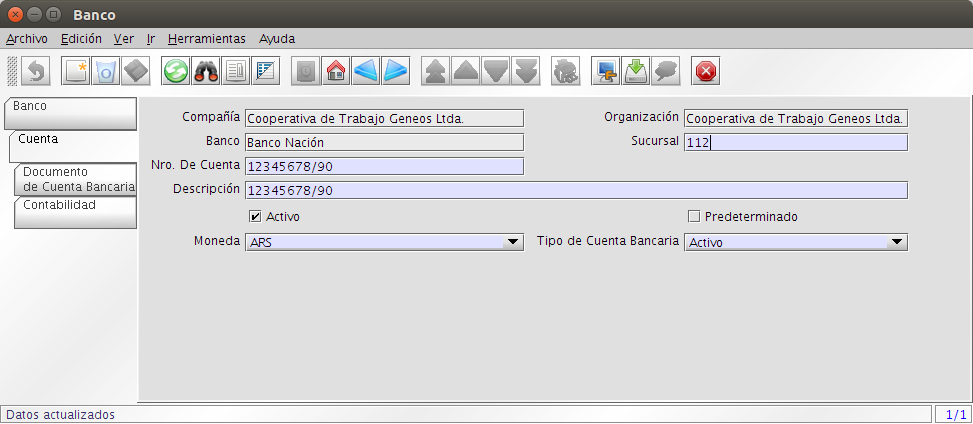
\includegraphics{ly_cuenta.png}
\caption{Imagen 6: Estructura de Ventanas - Pestaña}\end{figure}

En todas las ventanas de la aplicación se encontrara una estructura común en la parte superior. Por una parte, tenemos el menú compuesto por una serie de ventanas desplegables (Archivo, Edición, Ver, Ir, Herramientas, Ayuda).

Como ejemplo, dentro de Herramientas aparece la opción \textbf{Preferencias}. Las preferencias de usuario permite determinar la pantalla del cliente y como reaccionará ante específicas acciones de usuario. Sus opciones son las siguientes:
\begin{enumerate}
\item {} 
\textbf{Interfaz de Usuario:} El botón de interfaz de usuario permite la selección de la apariencia y estilo de Libertya. Se puede seleccionar diferentes estilos y colores y tener una vista previa de su selección antes de guardarla.

\item {} 
\textbf{Guardado Automático:} Si se selecciona Guardado Automático, los cambios se guardaran automáticamente cuando se navegue por una única pestaña. Cuando se cambien pestañas debe confirmar la acción independientemente de la opción.

\item {} 
\textbf{Acceso Automático:} Si se selecciona la casilla de verificación Acceso Automático, la ventana de Acceso no se mostrara cuando se inicie Libertya. Se usara el nombre de usuario, contraseña, perfil, cliente y organización de la sesión anterior. Si se quiere cambiar algún parámetro de estos debe bloquearse, quitando la selección de esta casilla de verificación y salir de Libertya. La próxima vez que se ingrese en la aplicación se mostrara la ventana de acceso y se podrá insertar los valores que se desee. Esta opción puede desactivarse para sistemas que requieran alta seguridad.

\item {} 
\textbf{Contraseña Almacenado:} Si se selecciona la casilla de verificación Recordar Contraseña, Libertya recordará el usuario y la contraseña con el que se accedió en la anterior sesión. Estos valores pueden ser sobrescritos fuera necesario.

\item {} 
\textbf{Mostrar Pestañas Contables / Mostrar Pestañas de Traducción:} Si se selecciona la casilla de verificación Mostrar Pestañas Contables / Mostrar Pestaña de Traducción, Libertya mostrará las pestañas contables y de traducción en aquellas ventana que contengan este tipo de pestañas.

\item {} 
\textbf{Traducción:} Las pestañas de traducción solo debería estar disponibles para los administradores de sistema, y las contables para el departamento de contabilidad o los usuarios debidamente cualificados para la parametrización de cuentas contables de la aplicación. Por esto, lo común será que los usuarios normales tengan estas dos casillas desactivadas y en modo de lectura solamente.

\item {} 
\textbf{Crear Objetos en el Servidor:} Se selecciona la casilla de verificación Crear Objetos en el Servidor solo si esta trabajando remotamente y se quiere reducir el tráfico de red. La contrapartida es que los objetos que son creados en el servidor requieren más recurso de servidor, por lo que puede ser necesario una mayor cantidad de memoria y de espacio de disco.

\item {} 
\textbf{Imprimir Siempre Vista Previa:} Si se selecciona esta casilla de verificación, Libertya mostrará una pantalla de Vista Previa antes de imprimir cualquier documento, informe o pantalla. Una vez visualizado, aprobado y validado dicho documento o informe se puede imprimir directamente.

\item {} 
\textbf{Nivel de Mensajes de Logs:} El nivel de depuración indica el nivel de detalle de los mensajes de la bitácora de errores, información e incidencias que genera Libertya en tiempo real. Se puede querer modificar esta opción cuando requiera soporte para un problema específico y el servicio de soporte solicite la información que esta opción proporciona. Esta utilidad no obstante, solo debería ser modificada por los administradores del sistema o usuarios profesionales debidamente cualificados que entiendan lo que están haciendo.

\item {} 
\textbf{Impresora:} Los campos de Impresión permiten seleccionar la impresora que será usada para los documentos e informes. Sobrescribirá el valor introducido o tomado por defecto cuando se inicio sesión en Libertya.

\item {} 
\textbf{Fecha:} El campo fecha permite seleccionar la fecha que será usada en los documentos. Sobrescribirá el valor entrado o tomado por defecto al iniciar la sesión de Libertya.

\end{enumerate}

Justo debajo se encuentra la barra de herramientas (botonera), con una serie de iconos comunes a todas las ventanas (crear, guardar, eliminar, buscar, imprimir, ver como grilla, etc). A continuación, en la ventana se encuentran los campos de la ventana, que permite visualizar y/o introducir nuevos datos dependiendo de la configuración en cada momento. Los campos en rojo deben contener obligatoriamente algún dato para poder guardar el registro. Para pasar de un campo a otro se realiza con el ratón o bien con la tecla Tab.
\begin{figure}[htbp]
\centering
\capstart


\includegraphics{ly_barra.png}
\caption{Imagen 7: Barra de Herramientas}\end{figure}

De izquierda a derecha:
\begin{enumerate}
\item {} 
Deshacer cambios

\item {} 
Nuevo registro

\item {} 
Eliminar registro

\item {} 
Guardar registro

\item {} 
Actualizar registro

\item {} 
Buscar registros

\item {} 
Adjuntos: permite adjuntar documentos a un registro de la ventana.

\item {} 
Vista:  formulario (ingreso de datos) y grilla (vista tipo tabla).

\item {} 
Historial de registros: en el caso de algunas ventanas los registros quedan ocultos tras un cierto tiempo de antigüedad para facilitar la navegación por la ventana. Con este botón se puede seleccionar la antigüedad de los registros que se muestran, pero solo en ese acceso a la ventana, cuando se vuelva a iniciar la ventana volverá a la vista original. Si siempre se desea ingresar con otro periodo de antigüedad, solo el administrador del sistema podrá configurarlo.

\item {} 
Inicio

\item {} 
Pestaña anterior

\item {} 
Pestaña siguiente

\item {} 
Primer registro

\item {} 
Registro anterior

\item {} 
Registro siguiente

\item {} 
Último registro

\item {} 
Imprimir (en los casos que la ventana lo permite)

\item {} 
Flujos de trabajo activos (en los contextos que tiene sentido)

\item {} 
Exportar

\item {} 
Conversación

\item {} 
Salir

\end{enumerate}


\chapter{Principales Maestros de la Aplicación}
\label{maestros:principales-maestros-de-la-aplicacion}\label{maestros::doc}\begin{itemize}
\item {} \begin{description}
\item[{Entidades Comerciales}] \leavevmode\begin{itemize}
\item {} 
Clientes

\item {} 
Proveedores

\item {} 
Empleados

\end{itemize}

\end{description}

\item {} 
Artículos

\item {} 
Conjuntos de Atributos

\item {} 
Lista de Precios

\end{itemize}


\section{Entidades Comerciales}
\label{maestros:entidades-comerciales}
Las entidades Comerciales se usan para ingresar al sistema Proveedores, Clientes y Empleados.

\textbf{Proveedores}
\begin{enumerate}
\item {} 
Acceder a la opción de menú \textbf{Entidades Comerciales \(\rightarrow\) Entidades Comerciales}, por defecto ingresa a la primera pestaña de \textbf{Entidad Comercial}, el sistema presenta una ventana como lo muestra la Imagen 8.

\item {} \begin{description}
\item[{Campos a ingresar:}] \leavevmode\begin{itemize}
\item {} 
Clave de Búsqueda (si no se ingresa el sistema genera una incremental).

\item {} 
Nombre.

\item {} 
Descripción.

\item {} 
Categoría de IVA

\item {} 
Tipo de Identificación

\item {} 
Número de Identificación

\item {} 
Grupo

\end{itemize}

\end{description}

\item {} 
Guardar

\item {} 
Seleccionar la pestaña \textbf{Proveedor}, el sistema presenta una ventana como lo muestra la Imagen 9.

\item {} \begin{description}
\item[{Campos a ingresar:}] \leavevmode\begin{itemize}
\item {} 
Marcar casilla de verificación Proveedor.

\item {} 
Seleccionar la Tarifa de Compras que corresponda.

\item {} 
Seleccionar la Forma de Pago que corresponda.

\item {} 
Seleccionar el Esquema de Descuentos que corresponda.

\item {} 
Seleccionar el Esquema de Vencimientos que corresponda.

\end{itemize}

\end{description}

\item {} 
Guardar

\item {} 
Seleccionar la pestaña \textbf{Contabilidad}.

\item {} \begin{description}
\item[{Campos a ingresar:}] \leavevmode\begin{itemize}
\item {} 
C x C de Proveedores: es la cuenta contable para los asientos de compras.

\end{itemize}

\end{description}

\item {} 
Guardar

\item {} 
Seleccionar pestaña \textbf{Localización}, el sistema presenta una ventana como lo muestra la Imagen 10.

\item {} \begin{description}
\item[{Campos a ingresar:}] \leavevmode\begin{itemize}
\item {} 
Ingresar los datos de la Dirección del Proveedor.

\end{itemize}

\end{description}

\item {} 
Guardar

\end{enumerate}
\begin{figure}[htbp]
\centering
\capstart

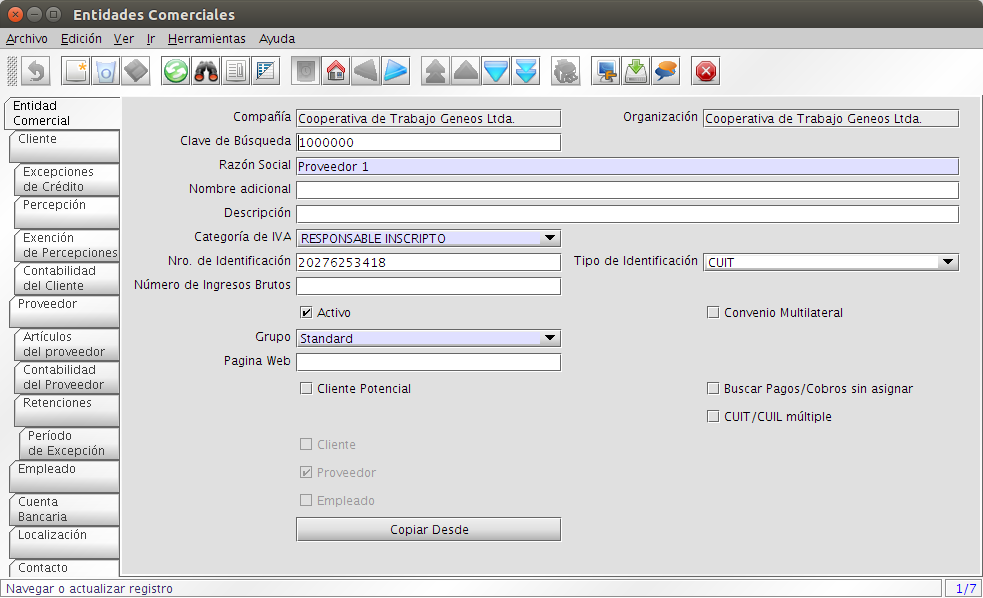
\includegraphics{ly_prov_gen.png}
\caption{Imagen 8: Entidades Comerciales}\end{figure}
\begin{figure}[htbp]
\centering
\capstart

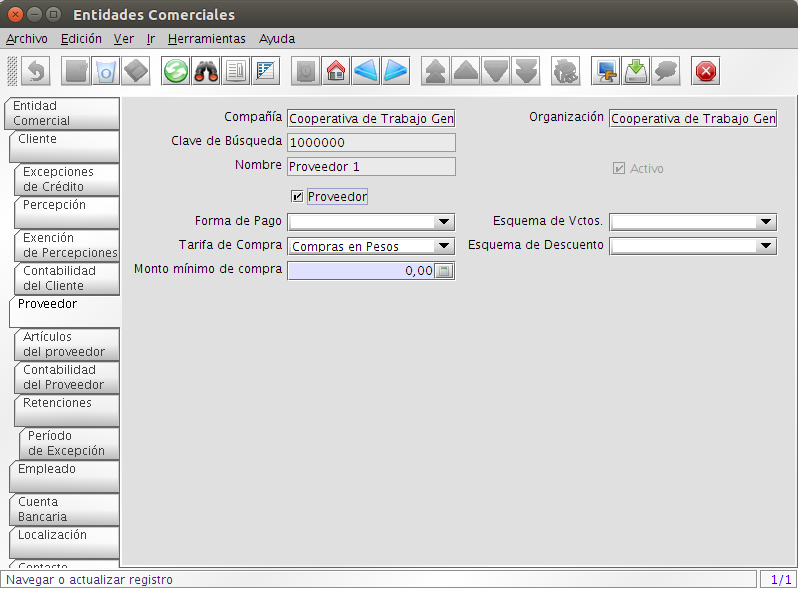
\includegraphics{ly_prov_prov.png}
\caption{Imagen 9: Entidades Comerciales - Proveedor}\end{figure}
\begin{figure}[htbp]
\centering
\capstart

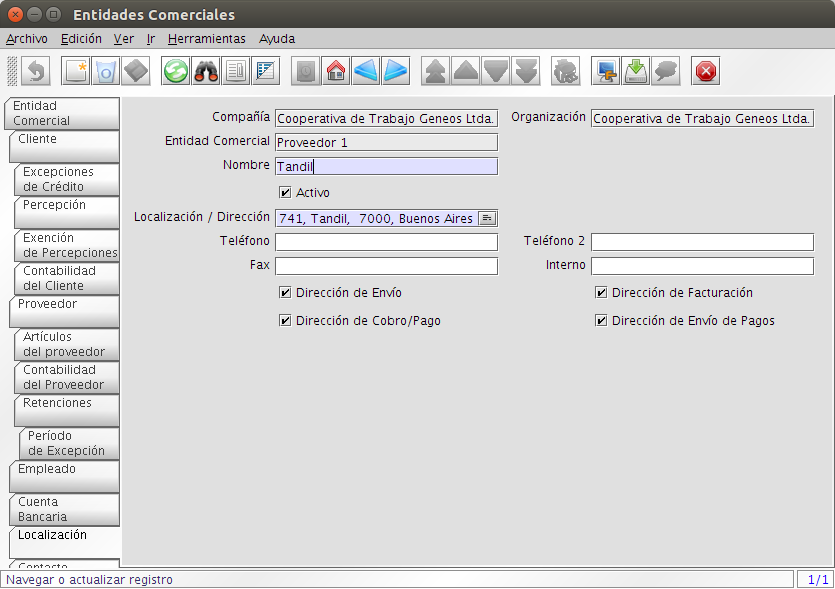
\includegraphics{ly_prov_dir.png}
\caption{Imagen 10: Entidades Comerciales - Localización}\end{figure}

\textbf{Clientes}
\begin{enumerate}
\item {} 
Acceder a la opción de menú \textbf{Entidades Comerciales \(\rightarrow\) Entidades Comerciales}, por defecto ingresa a la primera pestaña de \textbf{Entidad Comercial}, el sistema presenta una ventana como lo muestra la Imagen 8.

\item {} \begin{description}
\item[{Campos a ingresar:}] \leavevmode\begin{itemize}
\item {} 
Clave de Búsqueda (si no se ingresa el sistema genera una incremental).

\item {} 
Nombre.

\item {} 
Descripción.

\item {} 
Categoría de IVA

\item {} 
Tipo de Identificación

\item {} 
Número de Identificación

\item {} 
Grupo

\end{itemize}

\end{description}

\item {} 
Guardar.

\item {} 
Seleccionar la pestaña \textbf{Cliente}, el sistema presenta una ventana como lo muestra la Imagen 11.

\item {} \begin{description}
\item[{Campos a ingresar:}] \leavevmode\begin{itemize}
\item {} 
Marcar casilla de verificación Cliente.

\item {} 
Seleccionar el Estado de Crédito que corresponda.

\item {} 
Ingresar el Límite de Crédito que corresponda.

\item {} 
Seleccionar el Esquema de Descuentos que corresponda.

\item {} 
Seleccionar la Forma de Pago que corresponda.

\item {} 
Seleccionar el Medio de Cobro a Crédito que corresponda.

\end{itemize}

\end{description}

\item {} 
Guardar.

\item {} 
Seleccionar la pestaña \textbf{Contabilidad}.

\item {} \begin{description}
\item[{Campos a ingresar:}] \leavevmode\begin{itemize}
\item {} 
C x C de Clientes: es la cuenta contable para los asientos de ventas.

\end{itemize}

\end{description}

\item {} 
Guardar.

\item {} 
Seleccionar pestaña \textbf{Localización}, el sistema presenta una ventana como lo muestra la Imagen 10.

\item {} \begin{description}
\item[{Campos a ingresar:}] \leavevmode\begin{itemize}
\item {} 
Ingresar los datos de la Dirección del Proveedor.

\end{itemize}

\end{description}

\item {} 
Guardar.

\end{enumerate}
\begin{figure}[htbp]
\centering
\capstart

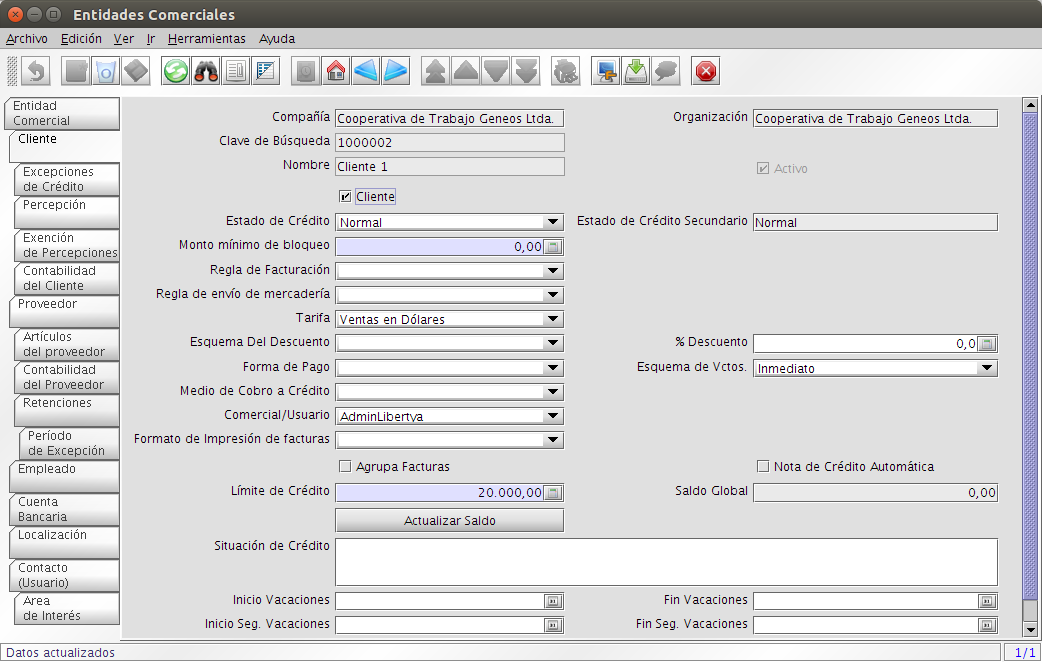
\includegraphics{ly_cli_cli.png}
\caption{Imagen 11: Entidades Comerciales - Cliente}\end{figure}

\textbf{Empleados}
\begin{enumerate}
\item {} 
Acceder a la opción de menú \textbf{Entidades Comerciales \(\rightarrow\) Entidades Comerciales}, por defecto ingresa a la primera pestaña de \textbf{Entidad Comercial}, el sistema presenta una ventana como lo muestra la Imagen 8.

\item {} \begin{description}
\item[{Campos a ingresar:}] \leavevmode\begin{itemize}
\item {} 
Clave de Búsqueda (si no se ingresa el sistema genera una incremental).

\item {} 
Nombre.

\item {} 
Descripción.

\item {} 
Categoría de IVA

\item {} 
Tipo de Identificación

\item {} 
Número de Identificación

\item {} 
Grupo

\end{itemize}

\end{description}

\end{enumerate}
\begin{enumerate}
\setcounter{enumi}{3}
\item {} 
Guardar

\item {} 
Seleccionar la pestaña \textbf{Empleado}, el sistema presenta una ventana como lo muestra la Imagen 12.

\item {} \begin{description}
\item[{Campos a ingresar:}] \leavevmode\begin{itemize}
\item {} 
Marcar casilla de verificación Empleado.

\end{itemize}

\end{description}

\item {} 
Guardar

\end{enumerate}
\begin{figure}[htbp]
\centering
\capstart

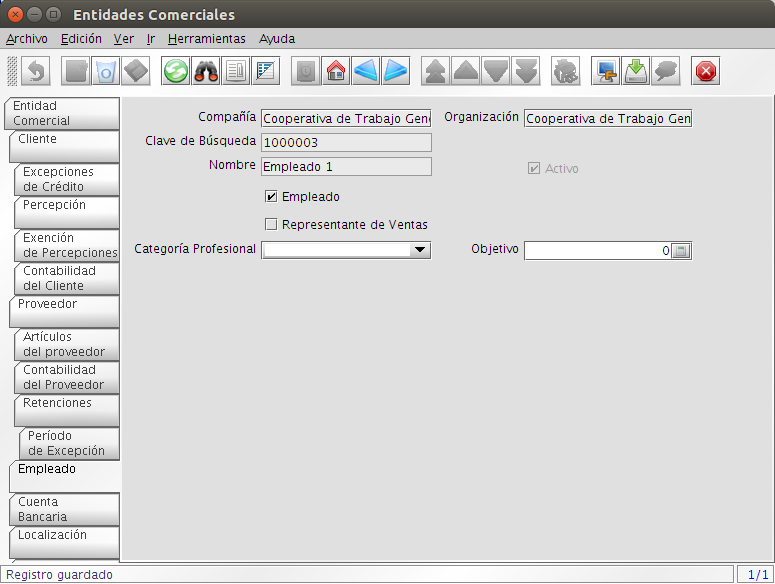
\includegraphics{ly_emp.png}
\caption{Imagen 12: Entidades Comerciales - Empleado}\end{figure}


\section{Artículos}
\label{maestros:articulos}
Los artículos o productos pueden ser aquellos vendibles a clientes, los usados en la fabricación de productos para venta a clientes, los productos comprados por una organización como materias primas, etc. También se utilizan artículos para facturar ítem especiales, en cuyos casos el tipo de artículo varía según la necesidad.
\begin{enumerate}
\item {} 
Acceder a la opción del menú \textbf{Artículos \(\rightarrow\)  Artículos}, por defecto ingresa a la primera pestaña de \textbf{Artículo}, el sistema presenta una ventana como lo muestra la Imagen 13.

\item {} \begin{description}
\item[{Campos a ingresar:}] \leavevmode\begin{itemize}
\item {} 
Nombre

\item {} 
Descripción.

\item {} 
UPC/EAN (Código de barra universal o número de artículo europeo), que con posterioridad permitirá una gestión rápida de stock mediante lectores de código de barra.

\item {} 
Subfamilia.

\item {} 
Marca.

\item {} 
Categoría de Impuesto

\item {} 
Tipo de Producto. Dependiendo de la selección de Tipo de Producto (que puede ser Artículo, Recurso, Servicio o Gasto) la ventana puede cambiar ligeramente.

\item {} 
UM es la Unidad de Medida en la que se almacenara este producto. Si se quiere hacer alguna conversión a otra Unidad de Medida, esta Unidad de Medida debe ser más pequeña. Por ejemplo, si se tiene un producto que puede venderse en unidades individuales o paquetes de 6 unidades, la UM definido para el producto deberá ser la unidad. Adicionalmente deberemos definir una conversión de unidades a paquetes de 6 unidades con una tasa de conversión multiplicadora de seis.

\item {} 
Seleccionar la casilla de Comprado y/o Vendido cuando la organización requiera comprar /vender este producto.

\end{itemize}

\end{description}

\item {} 
Guardar.

\item {} 
Seleccionar la pestaña \textbf{Precio}, el sistema presenta una ventana como lo muestra la Imagen 14.

\item {} \begin{description}
\item[{Campos a ingresar:}] \leavevmode\begin{itemize}
\item {} 
Versión de Tarifa

\item {} 
Precio Tarifa

\item {} 
Precio        Ref.

\item {} 
Precio Límite (en caso de querer controlar el precio por debajo del cual no puedan cargarse registros con el producto).

\end{itemize}

\end{description}

\item {} 
Guardar.

\item {} 
Seleccionar la pestaña \textbf{Contabilidad}, el sistema presenta una ventana como lo muestra la Imagen 15.

\item {} \begin{description}
\item[{Campos a ingresar:}] \leavevmode\begin{itemize}
\item {} 
Inventario de producto: es la cuenta contable para los asientos de ventas.

\item {} 
Discrepancia de producto: es la cuenta contable para los asientos de compras.

\end{itemize}

\end{description}

\item {} 
Guardar

\end{enumerate}
\begin{figure}[htbp]
\centering
\capstart

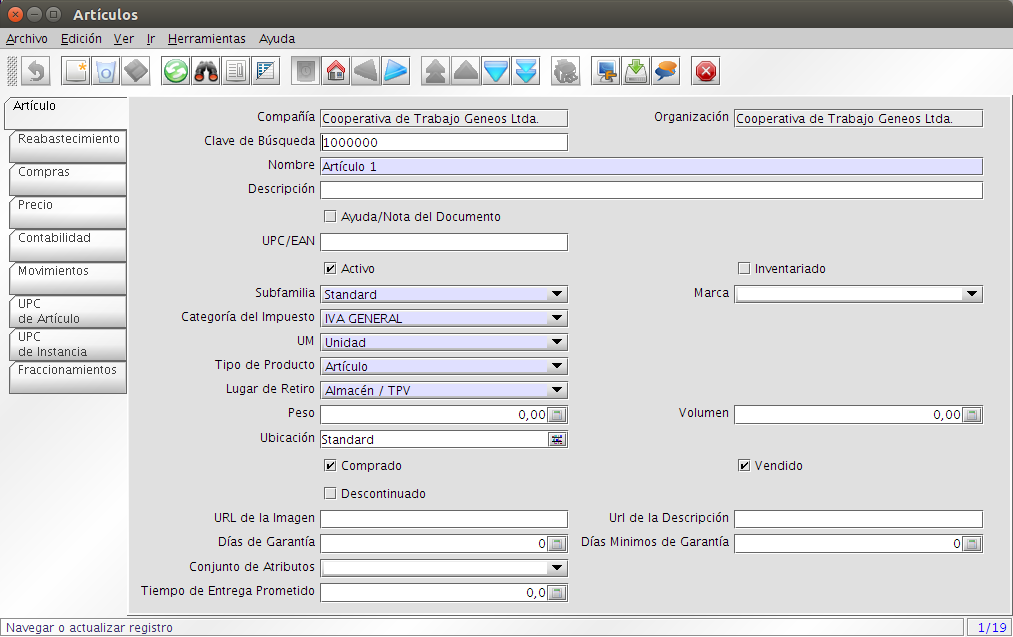
\includegraphics{ly_art_gen.png}
\caption{Imagen 13: Artículo - Datos Generales}\end{figure}
\begin{figure}[htbp]
\centering
\capstart

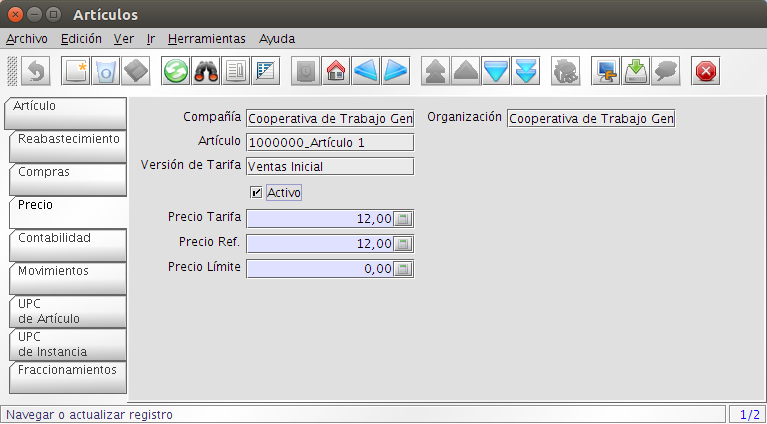
\includegraphics{ly_art_precio.png}
\caption{Imagen 14: Artículo - Datos de Compras}\end{figure}
\begin{figure}[htbp]
\centering
\capstart

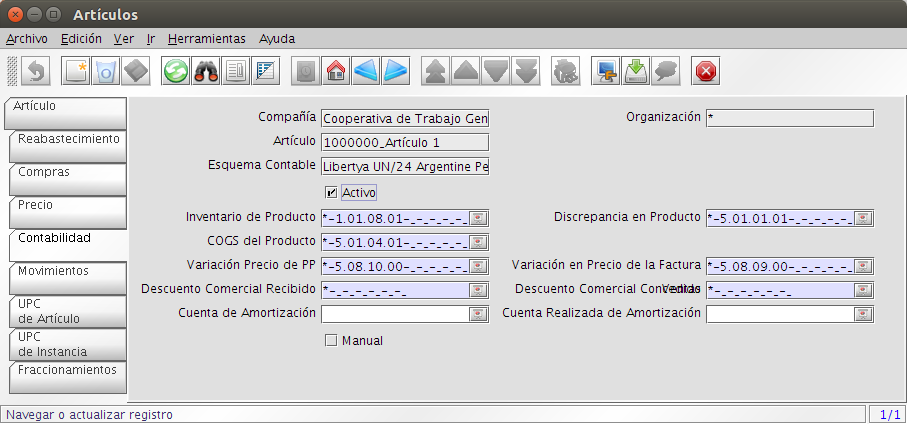
\includegraphics{ly_art_contab.png}
\caption{Imagen 15: Artículo - Datos Contabilidad}\end{figure}


\section{Conjunto de Atributos}
\label{maestros:conjunto-de-atributos}
Los Conjuntos de Atributos, permiten manejar características para diferenciar los lotes de productos y agregar características.

En el contexto del MRP, nos permite gestionar lotes de productos y vencimientos, de modo de poder hacer una trazabilidad, de los lotes que intervienen e cada proceso productivo.
\begin{enumerate}
\item {} 
Acceder a la opción del menú \textbf{Artículos \(\rightarrow\)  Atributos de Artículo}. Por defecto ingresa a la primera pestaña de \textbf{Conjunto de Atributos}, el sistema presenta una ventana como lo muestra la Imagen 16.

\item {} \begin{description}
\item[{Campos a ingresar:}] \leavevmode\begin{itemize}
\item {} 
Compañía:

\item {} 
Organización

\item {} 
Nombre

\item {} 
Descripción

\item {} 
Activo

\item {} 
Instancia del Atributo

\item {} 
Lote

\item {} 
Lote Obligatorio

\item {} 
Control de Lote

\item {} 
Nro de Serie

\item {} 
Nro de Serie Obligatorio

\item {} 
Control de Nro de Serie

\item {} 
Clave de relaciones de prod. prefijada

\item {} 
Fecha de Garantía

\item {} 
Fecha de Garantía Obligatoria

\item {} 
Días de Garantía

\item {} 
Tipo Obligatorio

\item {} 
Caduce

\end{itemize}

\end{description}

\end{enumerate}
\begin{enumerate}
\setcounter{enumi}{3}
\item {} 
Guardar.

\item {} 
En caso de requerir características particulares pueden definirse atributos por medio de la pestaña \textbf{Uso de Atributos}, el sistema presenta una ventana como lo muestra la Imagen 17.

\item {} \begin{description}
\item[{Campos a ingresar:}] \leavevmode\begin{itemize}
\item {} 
Compañía

\item {} 
Organización

\item {} 
Conjunto de Atributos

\item {} 
Atributo

\item {} 
Activo

\item {} 
Secuencia

\item {} 
Mostrado en descripción

\end{itemize}

\end{description}

\item {} 
Guardar.

\end{enumerate}
\begin{figure}[htbp]
\centering
\capstart

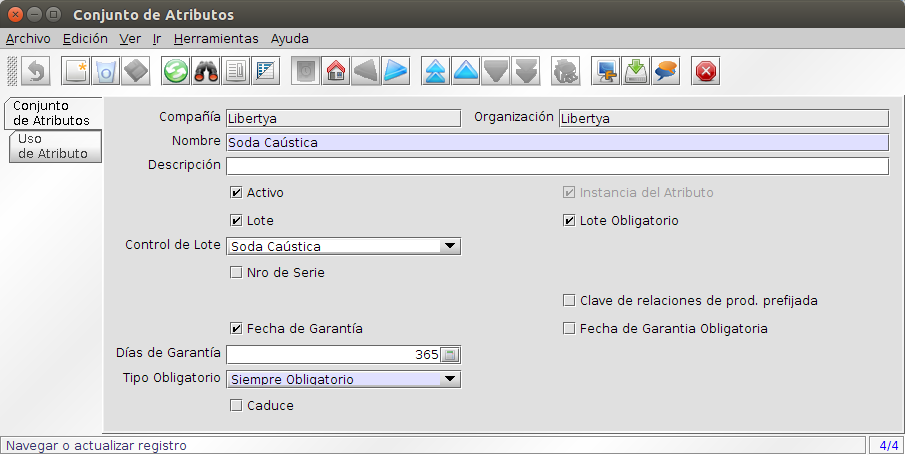
\includegraphics{ly_conjattr_1.png}
\caption{Imagen 16: Conjunto de Atributos}\end{figure}
\begin{figure}[htbp]
\centering
\capstart

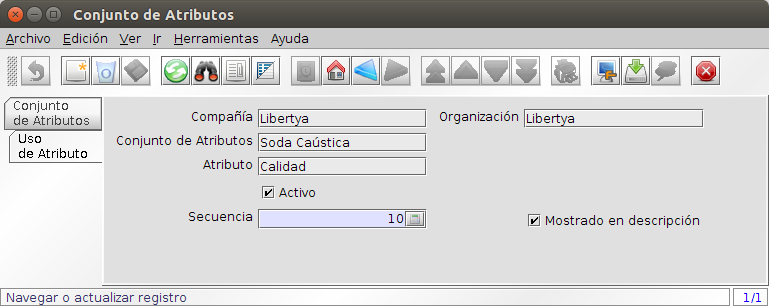
\includegraphics{ly_conjattr_2.png}
\caption{Imagen 17: Uso de Atributo}\end{figure}


\section{Control de Lote}
\label{maestros:control-de-lote}
Permite definir la gestión automática de numeración para los lotes.
\begin{enumerate}
\item {} 
Acceder a la opción del menú \textbf{Artículos \(\rightarrow\)  Atributos de Artículo \(\rightarrow\) Control de Lote del Artículo}. El sistema presenta una ventana como lo muestra la Imagen 18.

\item {} \begin{description}
\item[{Campos a ingresar:}] \leavevmode\begin{itemize}
\item {} 
Compañía

\item {} 
Organización

\item {} 
Nombre

\item {} 
Descripción

\item {} 
Activo

\item {} 
Nro. de Inicio

\item {} 
Incremento

\item {} 
Siguiente Secuencia

\item {} 
Prefijo

\item {} 
Sufijo

\end{itemize}

\end{description}

\item {} 
Guardar

\end{enumerate}
\begin{figure}[htbp]
\centering
\capstart

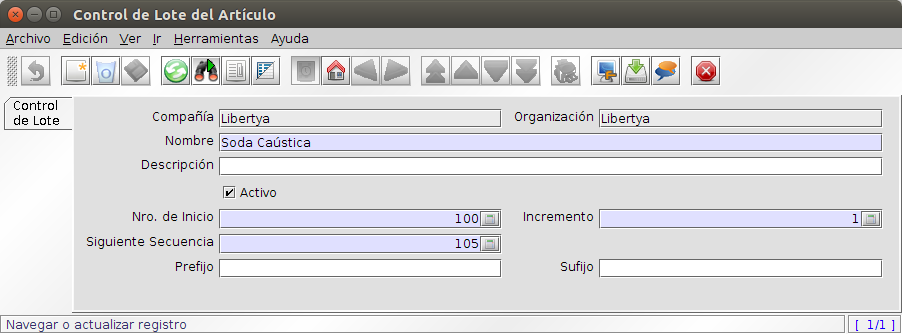
\includegraphics{ly_ctrlote.png}
\caption{Imagen 18: Control de Lote}\end{figure}


\section{Control de No de Serie}
\label{maestros:control-de-no-de-serie}
Permite definir la gestión automática de numeración para gestión de números de serie.
\begin{enumerate}
\item {} 
Acceder a la opción del menú \textbf{Artículos \(\rightarrow\)  Atributos de Artículo \(\rightarrow\) Control de No de Serie}. El sistema presenta una ventana como lo muestra la Imagen 19.

\item {} \begin{description}
\item[{Campos a ingresar:}] \leavevmode\begin{itemize}
\item {} 
Compañía

\item {} 
Organización

\item {} 
Nombre

\item {} 
Descripción

\item {} 
Activo

\item {} 
Nro. de Inicio

\item {} 
Incremento

\item {} 
Siguiente Secuencia

\item {} 
Prefijo

\item {} 
Sufijo

\end{itemize}

\end{description}

\item {} 
Guardar

\end{enumerate}
\begin{figure}[htbp]
\centering
\capstart

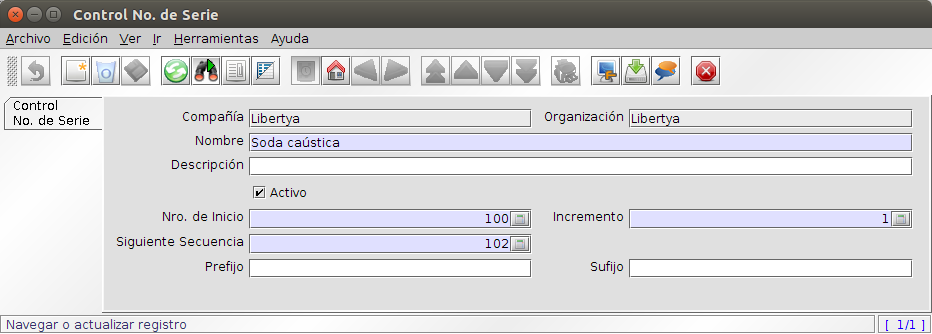
\includegraphics{ly_ctrserie.png}
\caption{Imagen 19: Control de No de Serie}\end{figure}


\section{Atributo}
\label{maestros:atributo}
Permite definir características particulares asociadas a un Conjunto de Atributos. Esto se hace definiendo una lista de posibles valores a ser seleccionados, asociada al atributo.
\begin{enumerate}
\item {} 
Acceder a la opción del menú \textbf{Artículos \(\rightarrow\) Atributos}. Por defecto ingresa a la primera pestaña de \textbf{Atributos}, el sistema presenta una ventana como lo muestra la Imagen 20.

\item {} \begin{description}
\item[{Campos a ingresar:}] \leavevmode\begin{itemize}
\item {} 
Compañía

\item {} 
Organización

\item {} 
Nombre

\item {} 
Descripción

\item {} 
Activo

\item {} 
Sólo Lectura

\item {} 
Tipo de Valor del Atributo

\item {} 
Entrada Obligatoria

\item {} 
Búsqueda por Atributo

\item {} 
Instancia del Atributo

\end{itemize}

\end{description}

\item {} 
Guardar.

\item {} 
Seleccionar la pestaña \textbf{Valor de Atributo}, el sistema presenta una ventana como lo muestra la Imagen 21.

\item {} \begin{description}
\item[{Campos a Ingresar:}] \leavevmode\begin{itemize}
\item {} 
Compañía

\item {} 
Organización

\item {} 
Atributo

\item {} 
Clave de Búsqueda

\item {} 
Nombre

\item {} 
Descripción

\item {} 
Activo

\item {} 
Secuencia

\end{itemize}

\end{description}

\item {} 
Guardar

\end{enumerate}
\begin{figure}[htbp]
\centering
\capstart

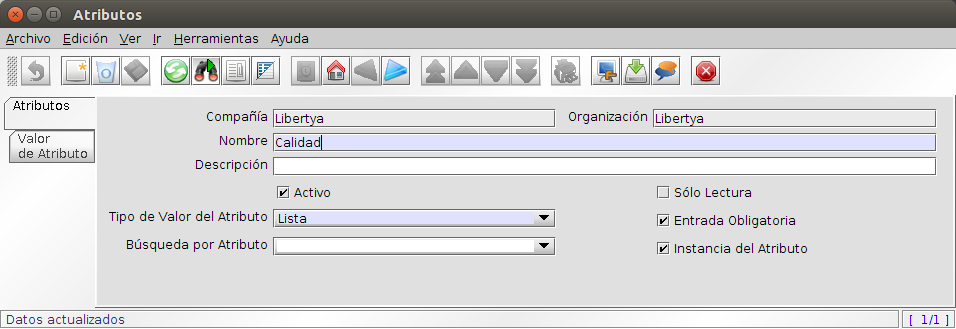
\includegraphics{ly_attr1.png}
\caption{Imagen 20: Artículo - Datos de Compras}\end{figure}
\begin{figure}[htbp]
\centering
\capstart

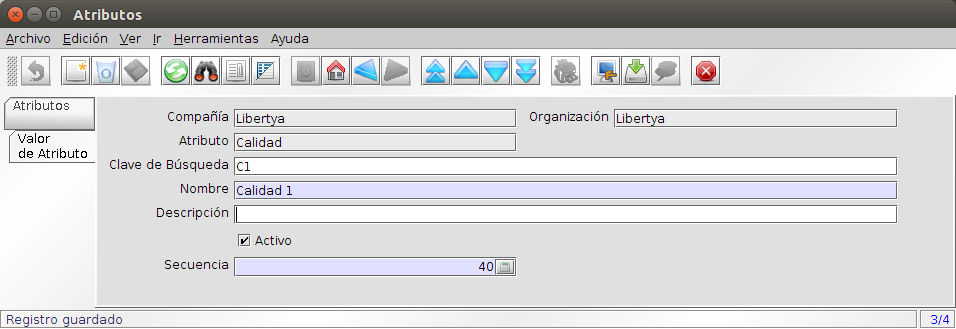
\includegraphics{ly_attr2.png}
\caption{Imagen 21: Artículo - Datos Contabilidad}\end{figure}


\chapter{Módulo de Compras}
\label{compras::doc}\label{compras:modulo-de-compras}
\textbf{Datos previos necesarios}
\begin{enumerate}
\item {} 
Clientes

\item {} 
Artículos

\item {} 
Lista de Precios de Compras

\item {} 
Medios de Cobro

\item {} 
Configuración de TPV

\item {} 
Viajes

\item {} 
Centros de Costos

\item {} 
Puntos de Viajes

\end{enumerate}


\chapter{Módulo de Ventas}
\label{ventas:modulo-de-ventas}\label{ventas::doc}
\textbf{Datos previos necesarios}
\begin{enumerate}
\item {} 
Clientes

\item {} 
Artículos

\item {} 
Lista de Precios de Compras

\item {} 
Medios de Cobro

\item {} 
Configuración de TPV

\item {} 
Centros de Costos

\end{enumerate}


\section{TPV}
\label{ventas:tpv}
La terminal de Punto de Venta (TPV) permite el ingreso rápido de las facturas de clientes.
\begin{figure}[htbp]
\centering
\capstart

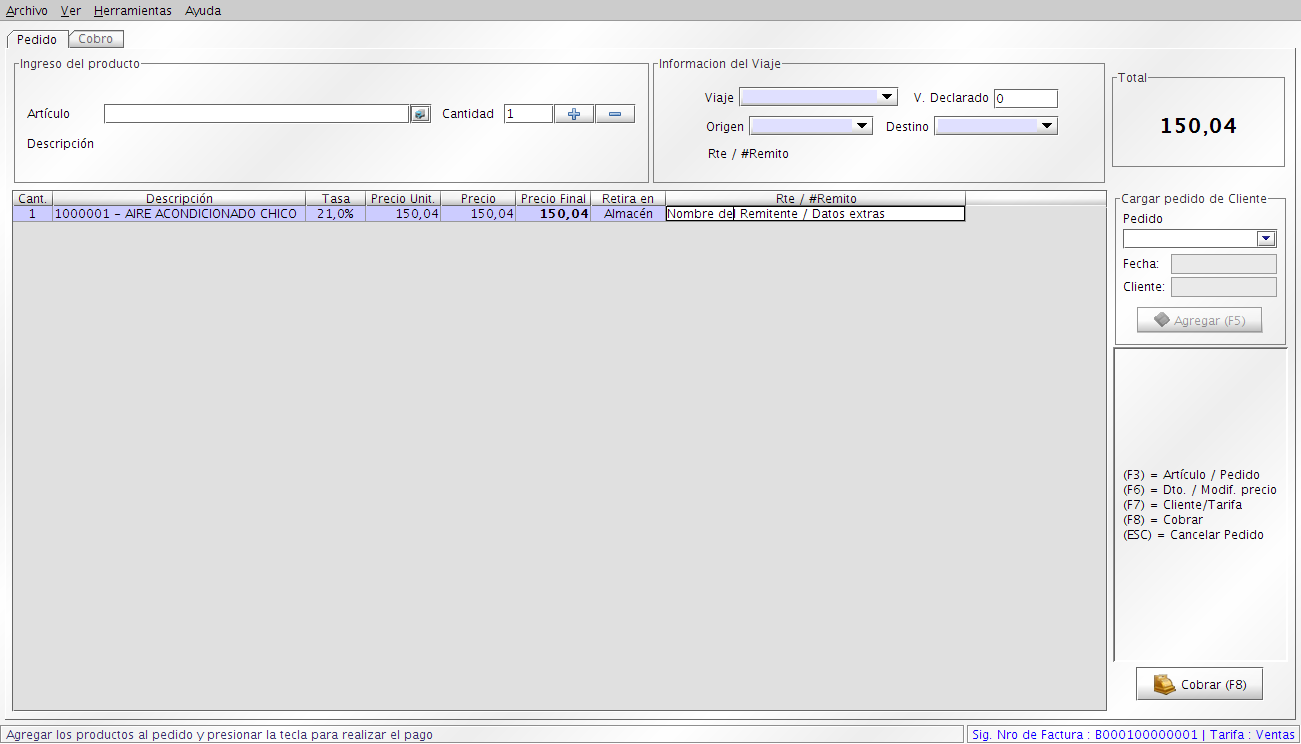
\includegraphics{ly_tpv_19.png}
\caption{Imagen 19: TPV – Ingreso de Ítem}\end{figure}

Acceder con el perfil ``Ventas'' a la opción del menú, menú TPV \(\rightarrow\)  TPV, el sistema presenta una ventana como lo muestra la Imagen 19.

Las referencias para el ingreso de la información de la compra son las siguientes:
\begin{enumerate}
\item {} 
Es el área de selección de los productos y cantidades (la tecla Intro sirve para fijar el producto y la cantidad ingresando la línea al pedido).

\item {} 
Es el área de ingreso del viaje, origen, destino (se mantienen los datos entre diferentes facturas, compartiendo los datos anteriormente registrados, para agilizar la carga de todas las facturas de un viaje) y valor declarado.

\item {} 
Es el área donde va quedando el detalle de las líneas de facturas, tiene una columna editable para ingresar la información de remitente asociada a cada línea.

\item {} 
Es el área de funciones:

\end{enumerate}
\begin{enumerate}
\item {} 
F6: para acceder a cambiar información de cantidades y precios de los productos.

\item {} 
F8: para cambiar a la pantalla de selección de Cliente y Medio de Pago. También puede usarse el botón Cobrar.

\end{enumerate}

La segunda parte de la transacción de ventas consiste en seleccionar el cliente y la forma de cobro.
\begin{enumerate}
\item {} 
Con el botón Cobrar o con F8 accedemos al siguiente paso de la factura que es la selección del Cliente y la Forma de Pago, el sistema presenta una ventana como lo muestra la Imagen 20.

\end{enumerate}
\begin{figure}[htbp]
\centering
\capstart

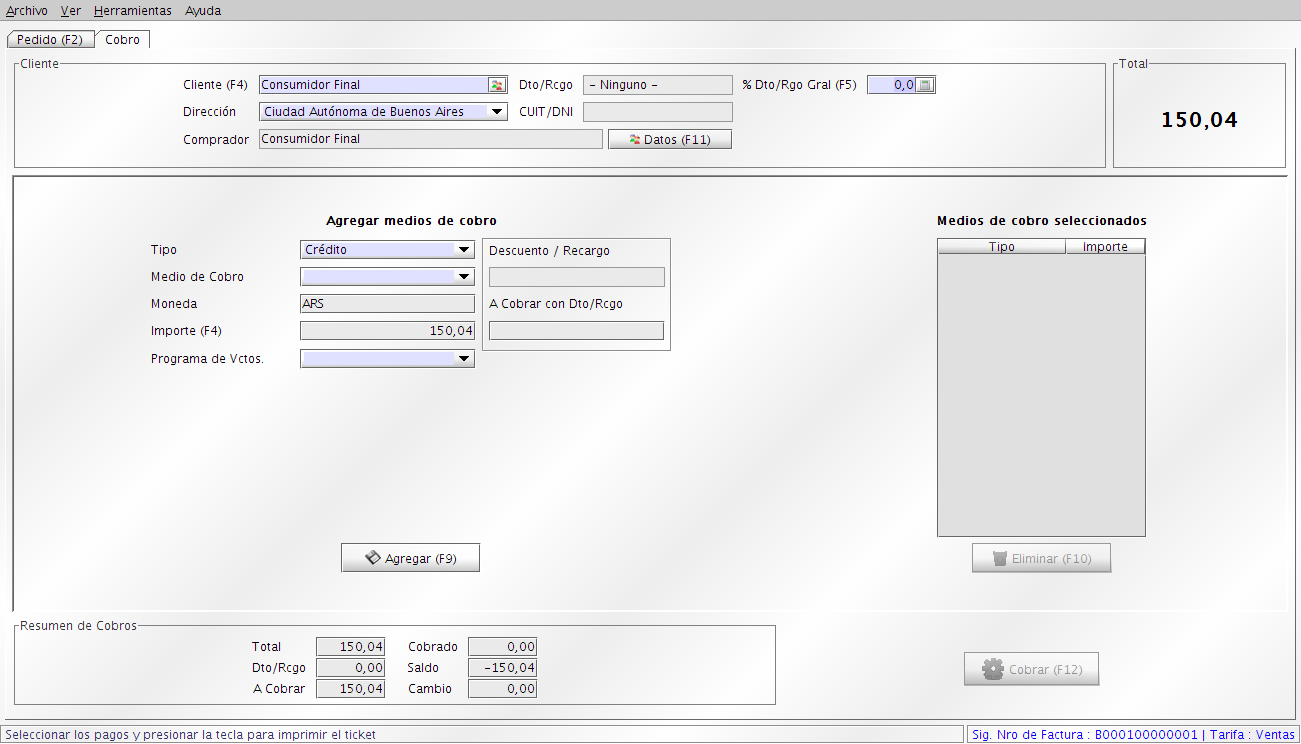
\includegraphics{ly_tpv_20.png}
\caption{Imagen 20: TPV – Ingreso de datos de Cobro}\end{figure}

Las referencias para el ingreso de la información del cliente y la forma de pago son las siguientes:
\begin{enumerate}
\item {} 
Es el área de selección del cliente. Se ingresa la información en el campo o se accede a la ventana de búsqueda.

\item {} 
Es el área de ingreso de la forma de cobro, en este caso siempre va a ser Crédito.

\item {} 
Acceso al botón para confirmar la operación (botón Cobrar o F12).

\end{enumerate}

Una vez confirmado el sistema emite el comprobante correspondiente.


\section{Cobranzas}
\label{ventas:cobranzas}
Permite registrar el cobro a un cliente.
\begin{enumerate}
\item {} 
Acceder con el perfil ``\textbf{Administración}'' a la opción del menú, menú Pagos \(\rightarrow\)  Orden de Pago, el sistema presenta una ventana como lo muestra la Imagen 21.

\item {} \begin{description}
\item[{\textbf{Cabecera} \(\rightarrow\) Campos a ingresar:}] \leavevmode\begin{itemize}
\item {} 
Entidad Comercial

\item {} 
Tipo de documento (determina el Nro. Documento)

\item {} 
Fecha del Recibo

\end{itemize}

\end{description}

\item {} \begin{description}
\item[{\textbf{Selección de Cobro} \(\rightarrow\) Campos a ingresar:}] \leavevmode\begin{itemize}
\item {} 
Seleccionar si es Cobro Normal o Cobro Adelantado (sin asignación de facturas)

\item {} 
Seleccionar Punto de Venta.

\item {} 
Seleccionar si se muestran todos los documentos o los vencidos a una fecha.

\item {} 
Indicar si se cobra todo lo pendiente o indicar en la columna a pagar el monto de la las facturas seleccionadas para pagar.

\item {} 
Con el botón Siguiente o F8 se avanza a la siguiente sección.

\end{itemize}

\end{description}

\item {} \begin{description}
\item[{\textbf{Forma de Cobro} (Imagen 22) \(\rightarrow\) Campos a ingresar:}] \leavevmode\begin{itemize}
\item {} 
Moneda

\item {} 
Tipo de Cobro/Pago

\item {} 
Datos correspondientes al tipo de cobro.

\item {} 
Guardar Cambios o F9

\end{itemize}

Repetir los últimos dos pasos en casos de cobrar con diferentes medios de cobro.
Una vez que el Saldo sea 0 completa con el botón \textbf{Emitir Recibo} o F8

\end{description}

\end{enumerate}
\begin{figure}[htbp]
\centering
\capstart

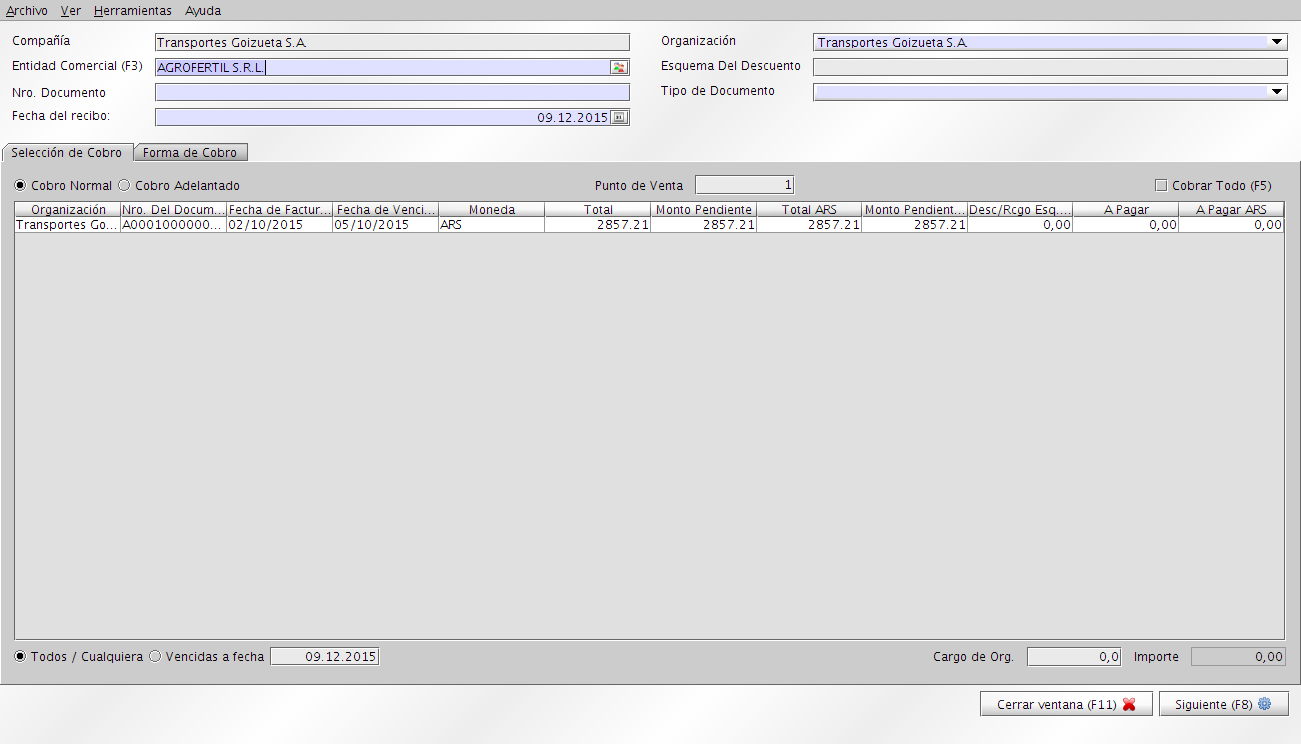
\includegraphics{ly_ventas21.png}
\caption{Imagen 21: Cobranzas – Ingreso de comprobantes a cobrar}\end{figure}
\begin{figure}[htbp]
\centering
\capstart

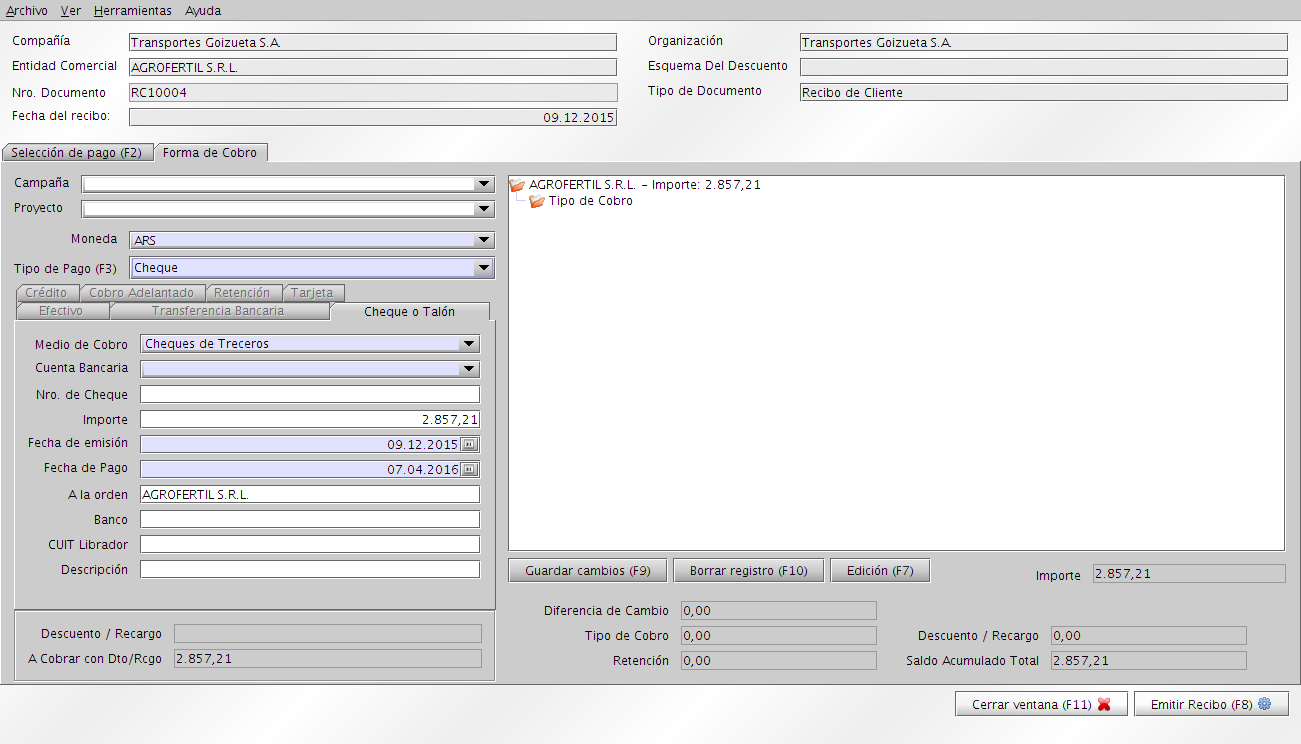
\includegraphics{ly_ventas22.png}
\caption{Imagen 22: Cobranzas – Ingreso de medios de cobro}\end{figure}


\section{Informes}
\label{ventas:informes}
\textbf{Cuenta Corriente}

Permite ver la información consolidada, de la cuenta corriente de un Cliente.
\begin{enumerate}
\item {} 
Acceder con el perfil ``Administración'' a la opción del menú, menú Informes de Cobros y Pagos \(\rightarrow\)  Informe de Cuenta Corriente, el sistema presenta una ventana como lo muestra la Imagen 23.

\item {} \begin{description}
\item[{Parámetros del informe (Imagen 23) \(\rightarrow\) Campos a ingresar:}] \leavevmode\begin{itemize}
\item {} 
Entidad Comercial

\item {} 
Organización (por defecto lo que viene)

\item {} 
Rango de Fechas

\item {} 
Tipo de Documentos

\item {} 
Tipo de Reporte (Cliente / Proveedor)

\end{itemize}

\end{description}

\item {} 
Emitir informe (Imagen 24) con el botón verde.

\end{enumerate}
\begin{figure}[htbp]
\centering
\capstart

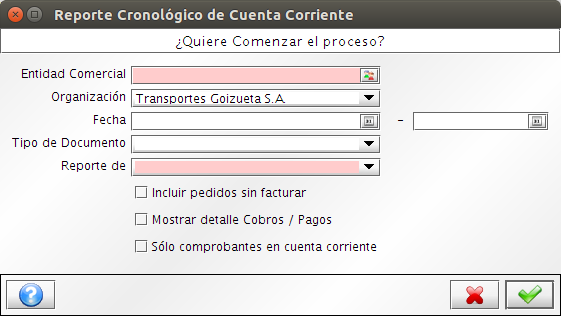
\includegraphics{ly_informe_23.png}
\caption{Imagen 23: Informe de Cta. Cte. - Parámetros}\end{figure}
\begin{figure}[htbp]
\centering
\capstart

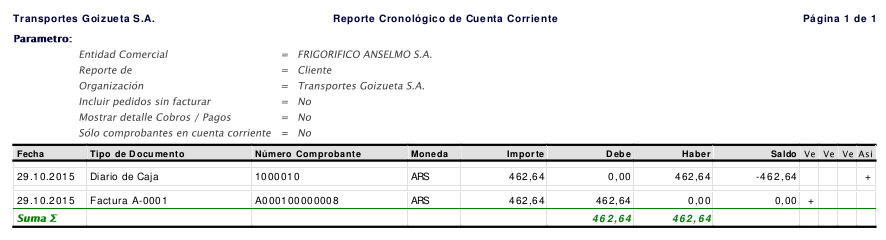
\includegraphics{ly_informe_24.png}
\caption{Imagen 24: Informe de Cta. Cte. - Resultados}\end{figure}


\chapter{Módulo de Finanzas}
\label{finanzas:modulo-de-finanzas}\label{finanzas::doc}

\section{Bancos}
\label{finanzas:bancos}
Desde esta ventana se configuran todas las cuentas bancarias con las que vaya a trabajar la compañía. En la primera pestaña se definirán los datos generales de la cuenta bancaria, su nombre, dirección, etc.

Adicionalmente se se activa la selección de Banco Propio, se podrá utilizar para las operaciones bancarias de cobros y pagos de la propia compañía. Donde podemos operar con varios bancos y cuentas a la vez.
\begin{enumerate}
\item {} 
Acceder con el perfil ``Administración'' a la opción del menú, \textbf{Banco} \(\rightarrow\)  \textbf{Banco}, el sistema presenta una ventana como lo muestra la Imagen 25.

\item {} \begin{description}
\item[{Datos Generales \(\rightarrow\) Campos a ingresar:}] \leavevmode\begin{itemize}
\item {} 
Nombre

\item {} 
Descripción

\item {} 
Dirección

\item {} 
Identificador

\end{itemize}

\end{description}

\end{enumerate}
\begin{figure}[htbp]
\centering
\capstart

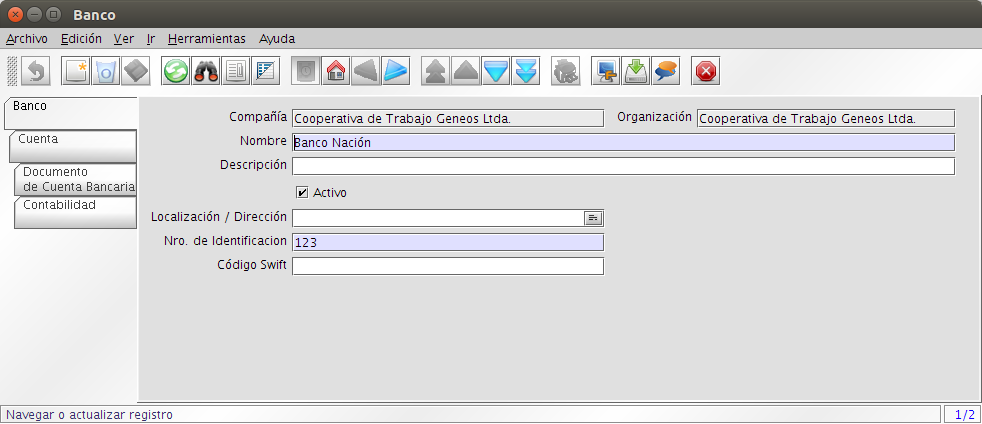
\includegraphics{ly_bancos_25.png}
\caption{Imagen 25: Bancos}\end{figure}

\textbf{Cuenta}
\begin{enumerate}
\item {} 
Acceder a la pestaña Cuenta, el sistema presenta una ventana como lo muestra la Imagen 26.

\item {} \begin{description}
\item[{Datos Generales \(\rightarrow\) Campos a ingresar:}] \leavevmode\begin{itemize}
\item {} 
Sucursal.

\item {} 
Nro. Cuenta.

\item {} 
Moneda.

\item {} 
Tipo de cuenta bancaria.

\item {} 
Cuenta de Cheques en Cartera, se habilita si el tipo de cuenta es Cheque, sirve para definir las cuentas que van a funcionar para mantener la cartera de cheques de Terceros.

\end{itemize}

\end{description}

\end{enumerate}
\begin{figure}[htbp]
\centering
\capstart

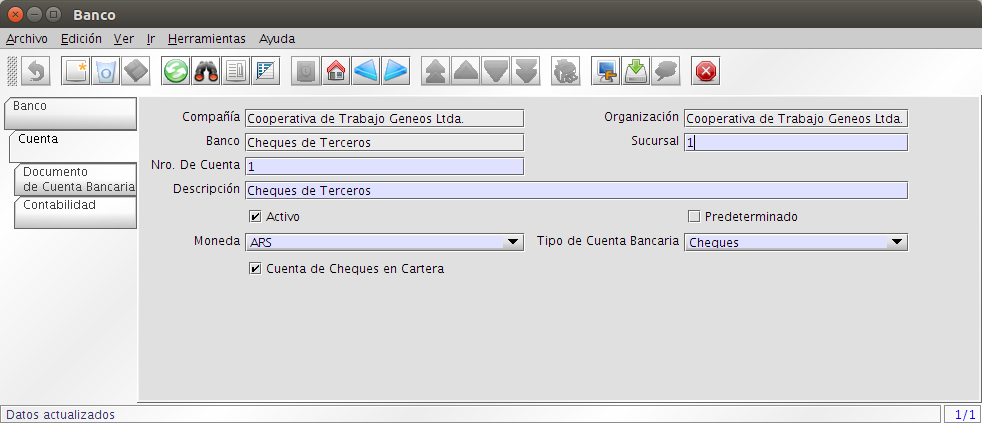
\includegraphics{ly_bancos_26.png}
\caption{Imagen 26: Cuentas}\end{figure}

\textbf{Documentos de Cuenta Bancarias}

Se usan para definir las chequeras en las cuentas de cheques propios.
\begin{enumerate}
\item {} 
Acceder a la pestaña \textbf{Documento de Cuenta Bancaria}, el sistema presenta una ventana como lo muestra la Imagen 27.

\item {} \begin{description}
\item[{Datos Generales \(\rightarrow\) Campos a ingresar:}] \leavevmode\begin{itemize}
\item {} 
Nombre.

\item {} 
Forma de Pago.

\item {} 
Secuencia.

\end{itemize}

\end{description}

\end{enumerate}
\begin{figure}[htbp]
\centering
\capstart

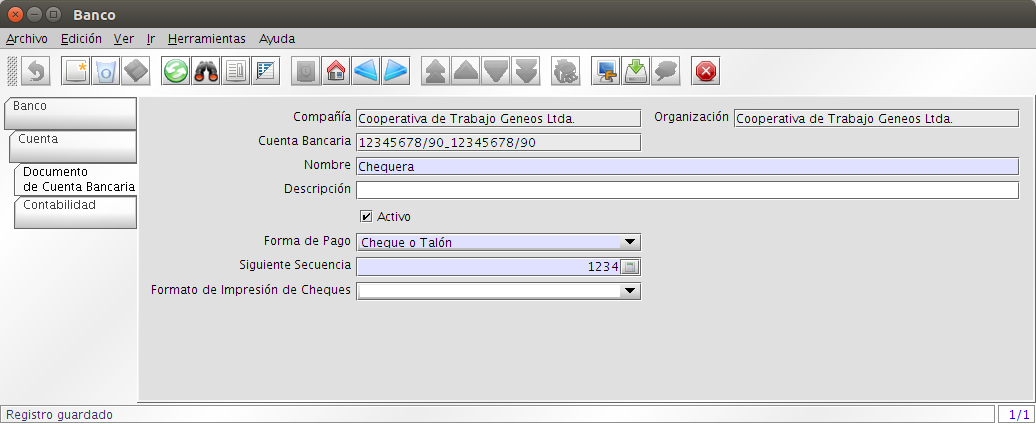
\includegraphics{ly_bancos_27.png}
\caption{Imagen 27: Documento de Cuenta Bancaria}\end{figure}


\section{Operaciones con Bancos}
\label{finanzas:operaciones-con-bancos}
\textbf{Transferencias Bancarias}

Permite realizar transferencias desde cuentas de terceros a cuentas propias, desde cuentas propias a cuentas de terceros y entre cuentas propias.
\begin{enumerate}
\item {} 
Acceder con el perfil ``\textbf{Administración}'' a la opción del menú, \textbf{Banco} \(\rightarrow\)  \textbf{Transferencia Bancaria}, el sistema presenta una ventana como lo muestra la Imagen 28.

\item {} \begin{description}
\item[{Datos Generales \(\rightarrow\) Campos a ingresar:}] \leavevmode\begin{itemize}
\item {} 
Fecha.

\item {} 
Entidad Comercial.

\item {} 
Cuenta Origen.

\item {} 
Cuenta Destino.

\item {} 
Importe.

\end{itemize}

\end{description}

\end{enumerate}
\begin{figure}[htbp]
\centering
\capstart

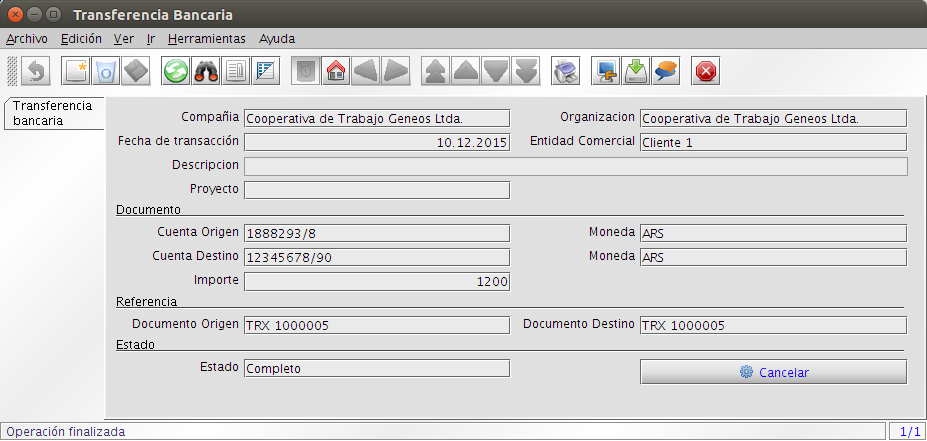
\includegraphics{ly_bancos_28.png}
\caption{Imagen 28: Transferencia Bancaria}\end{figure}

\textbf{Boleta de Depósitos}

Permite hacer el depósito de valores a una cuenta bancaria propia o de terceros. Primero se ingresan los datos generales y luego se ingresan los valores a depositar.
\begin{enumerate}
\item {} 
Acceder con el perfil ``Administración'' a la opción del menú, Banco \(\rightarrow\)  Boletas de Depósito, el sistema presenta una ventana como lo muestra la Imagen 29.

\item {} \begin{description}
\item[{Datos Generales \(\rightarrow\) Campos a ingresar:}] \leavevmode\begin{itemize}
\item {} 
Nro. de Documento (lo puede dar automático el sistema)

\item {} 
Entidad Comercial.

\item {} 
Cuenta Bancaria.

\item {} 
Fecha de Depósito.

\item {} 
Fecha de Acreditación.

\item {} 
Moneda.

\item {} 
Acción.

\end{itemize}

\end{description}

\end{enumerate}
\begin{figure}[htbp]
\centering
\capstart

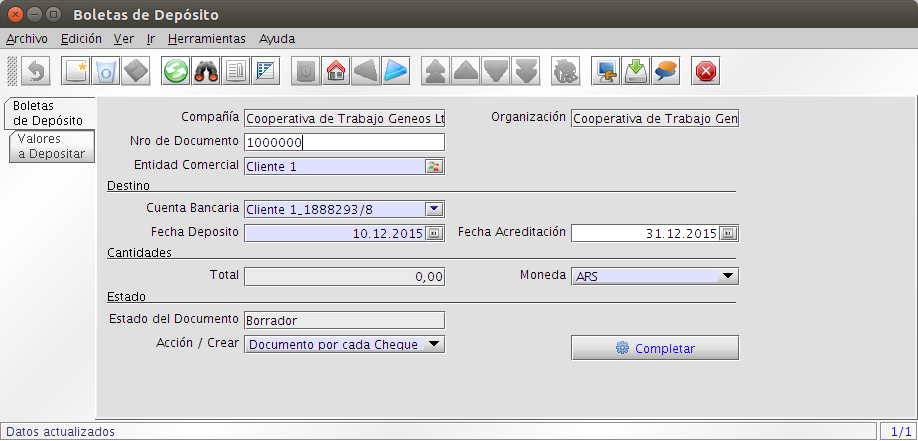
\includegraphics{ly_bancos_29.png}
\caption{Imagen 29: Boleta de Depósito - Datos generales}\end{figure}

\textbf{Valores a Depositar}
\begin{enumerate}
\item {} 
Acceder a la pestaña Valores a Depositar, el sistema presenta una ventana como lo muestra la Imagen 30. El ingreso de los valores actualiza el monto de la cabecera de la boleta.

\item {} \begin{description}
\item[{Campos a ingresar:}] \leavevmode\begin{itemize}
\item {} 
Cuenta origen.

\item {} 
Cheque.

\end{itemize}

\end{description}

\end{enumerate}
\begin{figure}[htbp]
\centering
\capstart

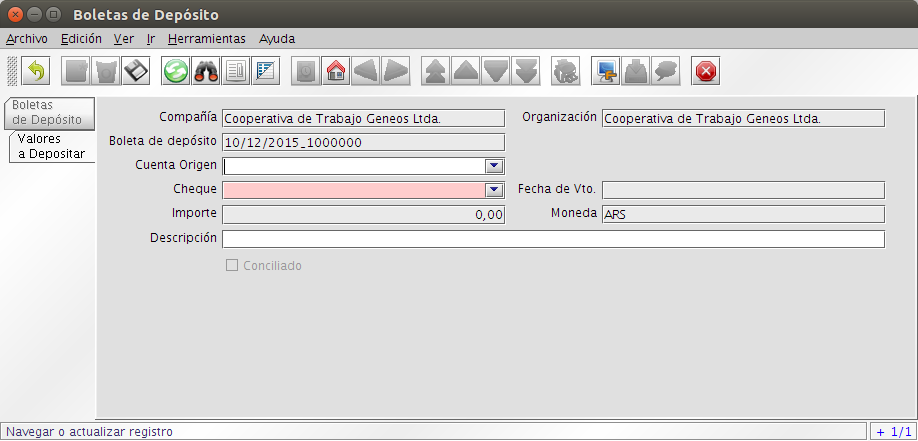
\includegraphics{ly_bancos_30.png}
\caption{Imagen 30: Boleta de Depósito - Valores a depositar}{\small 
Cajas
}\end{figure}


\bigskip\hrule{}\bigskip


\textbf{Configuración de Libro de Caja}

Define la estructura general de los tipos de cajas diarias.
\begin{enumerate}
\item {} 
Acceder con el perfil ``\textbf{Administración}'' a la opción del menú, \textbf{Caja} \(\rightarrow\)  \textbf{Configuración de Libro de Caja}, el sistema presenta una ventana como lo muestra la Imagen 31.

\item {} \begin{description}
\item[{Datos Generales \(\rightarrow\) Campos a ingresar:}] \leavevmode\begin{itemize}
\item {} 
Nombre.

\item {} 
Descripción.

\item {} 
Moneda.

\item {} 
Predeterminado.

\item {} 
Tipo de Caja, en esta instancia trabajamos siempre con el tipo Caja General.

\end{itemize}

\end{description}

\end{enumerate}
\begin{figure}[htbp]
\centering
\capstart

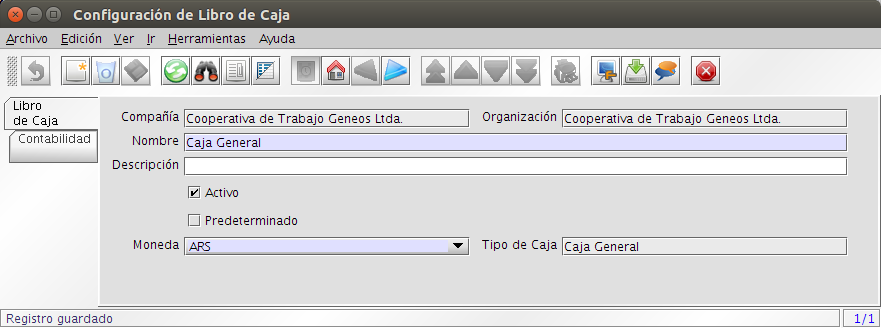
\includegraphics{ly_cajas_31.png}
\caption{Imagen 31: Configuración de Libro de Caja}\end{figure}

\textbf{Libro de Caja}

El libro de caja es donde se maneja el efectivo. Aquí se pueden registrar los ingresos y egresos de efectivo, ingresos de cheques y demás. Por ejemplo, si se paga una factura en efectivo, se debe crear una línea con la factura y el importe, para que se registre la cancelación de la misma.
\begin{enumerate}
\item {} 
Acceder con el perfil ``\textbf{Administración}'' a la opción del menú, \textbf{Caja} \(\rightarrow\)  \textbf{Libro de Caja}, el sistema presenta una ventana como lo muestra la Imagen 32.

\item {} \begin{description}
\item[{Datos Generales \(\rightarrow\) Campos a ingresar:}] \leavevmode\begin{itemize}
\item {} 
Libro de Caja.

\item {} 
Nombre, es asignado por el sistema con la referencia del Libro de Caja y la fecha, pero puede modificarse

\item {} 
Fecha de Estado de Cuenta.

\item {} 
Fecha de Aplicación CG (Contabilidad General).

\item {} 
Saldo Inicial, se carga de forma automática con el saldo de la última caja cerrada.

\item {} 
Completar, es la opción para cerrar el Libro de Caja y completar las transacciones.

\end{itemize}

\end{description}

\end{enumerate}
\begin{figure}[htbp]
\centering
\capstart

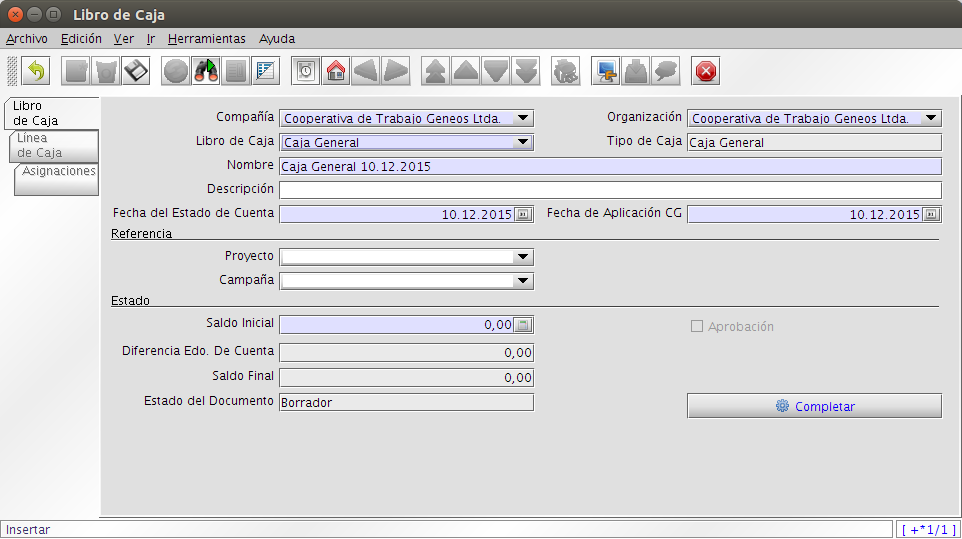
\includegraphics{ly_cajas_32.png}
\caption{Imagen 32: Libro de Caja}\end{figure}

Línea de Caja

Permite el ingreso de transacciones de caja. Los tipos que soporta son:

Gastos Generales, permite registrar gastos o egresos sin comprobantes.
Cobros Generales, permite registrar cobros o ingresos sin comprobantes.
Diferencia de Caja
Transferencia a Caja, permite transferir fondos desde una cuenta a la caja.
Transferencia a Cuenta Bancaria, permite transferir fondos desde la caja a una cuenta.
Factura, permite registrar el pago o la cobranza de facturas en efectivo.
\begin{enumerate}
\item {} 
Acceder a la pestaña Línea de Caja, el sistema presenta una ventana como lo muestra la Imagen 33.

\item {} \begin{description}
\item[{Datos Generales \(\rightarrow\) Campos a ingresar:}] \leavevmode\begin{itemize}
\item {} 
Descripción.

\item {} 
Entidad Comercial.

\item {} 
Tipo de Efectivo.

\item {} 
Importe.

\item {} 
Completar, es la opción para cerrar el registro en la Línea de Caja y completar la transacción.

\end{itemize}

\end{description}

\end{enumerate}
\begin{figure}[htbp]
\centering
\capstart

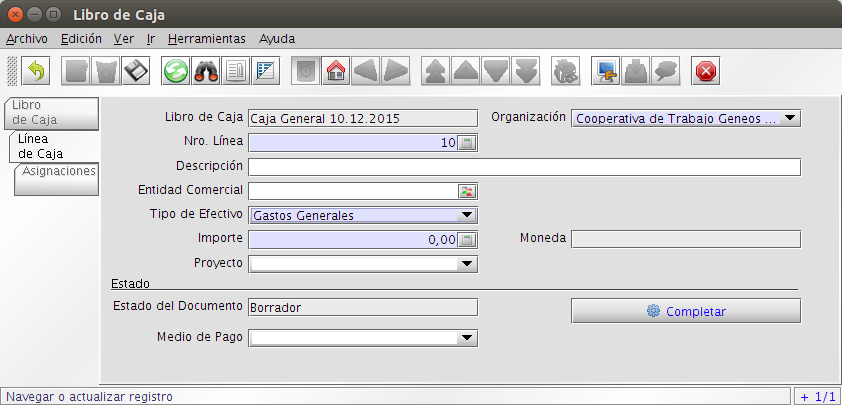
\includegraphics{ly_cajas_33.png}
\caption{Imagen 33: Línea de Caja}\end{figure}


\section{Operaciones con Cajas}
\label{finanzas:operaciones-con-cajas}
\textbf{Gastos Generales}

Permite registrar gastos o egresos sin comprobantes.
\begin{figure}[htbp]
\centering
\capstart

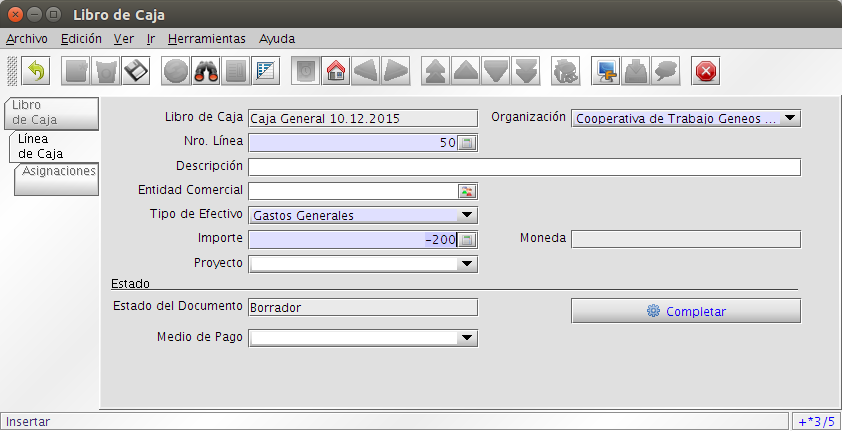
\includegraphics{ly_cajas_34.png}
\caption{Imagen 34: Linea de Caja – Gastos Generales}\end{figure}

\textbf{Cobros Generales}

Permite registrar cobros o ingresos sin comprobantes.
\begin{figure}[htbp]
\centering
\capstart

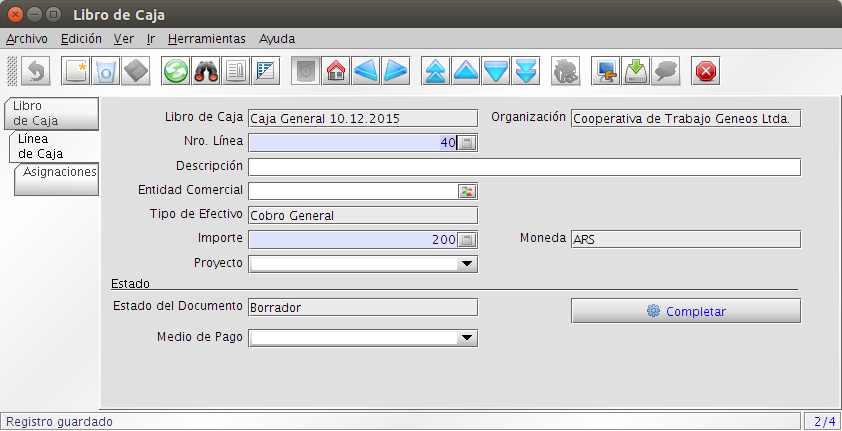
\includegraphics{ly_cajas_35.png}
\caption{Imagen 35: Linea de Caja – Cobros Generales}\end{figure}

\textbf{Diferencia de Caja}

Permite registrar diferencias de efectivo.
\begin{figure}[htbp]
\centering
\capstart

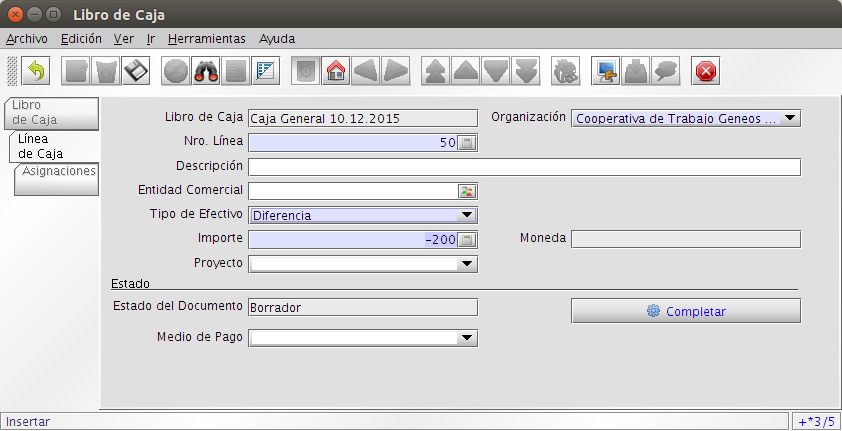
\includegraphics{ly_cajas_36.png}
\caption{Imagen 36: Linea de Caja – Diferencias de Efectivo}\end{figure}

\textbf{Transferencia a Caja}

Permite transferir fondos desde un Libro de Caja activo a otro.
\begin{figure}[htbp]
\centering
\capstart

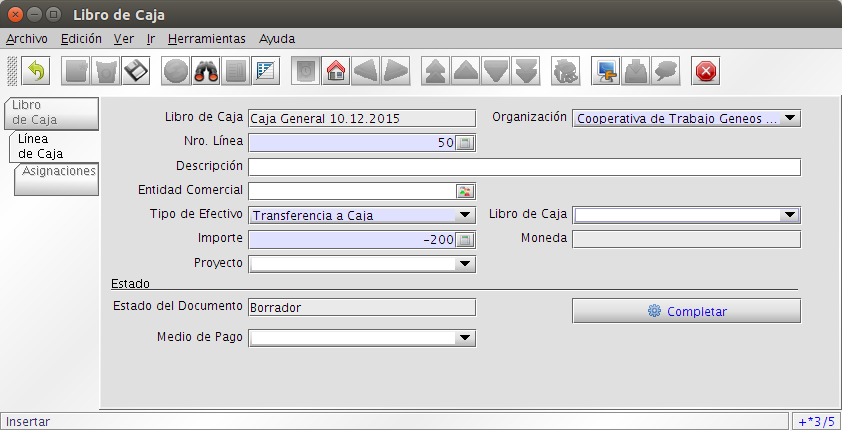
\includegraphics{ly_cajas_37.png}
\caption{Imagen 37: Linea de Caja – Transferencias entre Libros de Caja}\end{figure}

\textbf{Transferencia a Cuenta Bancaria}

Permite transferir fondos desde o hacia una cuenta bancaria.
\begin{figure}[htbp]
\centering
\capstart

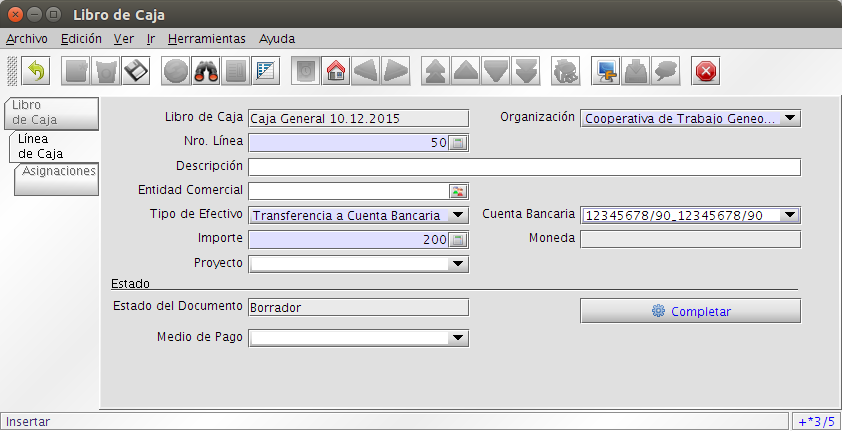
\includegraphics{ly_cajas_38.png}
\caption{Imagen 38: Linea de Caja – Transferencias entre Libros de Caja}\end{figure}

\textbf{Factura}

Permite registrar el pago o la cobranza de facturas en efectivo.
\begin{quote}
\begin{figure}[htbp]
\centering
\capstart

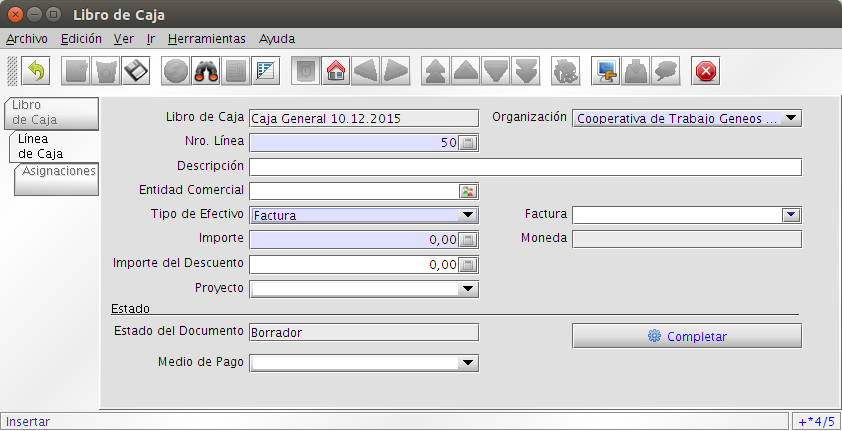
\includegraphics{ly_cajas_39.png}
\caption{Imagen 39: Linea de Caja – Cobranzas o Pagos de facturas en efectivo.}\end{figure}
\end{quote}


\chapter{Módulo de Contabilidad}
\label{contabilidad::doc}\label{contabilidad:modulo-de-contabilidad}

\section{Información General}
\label{contabilidad:informacion-general}
Un Esquema Contable es una combinación de los principios contables estándar nacionales, un método de coste y una moneda.

No hay que preocuparse acerca de que elementos introducir con cada transacción,  Libertya genera todas las operaciones contables automáticamente ya que las cuentas de derivan de la operación del documento. Para esto, el Esquema Contable define las cuentas por defecto para uso en transacciones generadas por el sistema. Ejemplo contabilidad de las facturas.

Estas cuentas se usan como valor por defecto para las Entidades Comerciales, Almacenes, Proyectos, Banco, Impuesto y Libro de Caja. Puede ser cambiadas a nivel individual.

El objetivo es generar todos los registros contables. Consecuentemente, todas las
cuentas necesarias están predeterminadas. Por ejemplo, si se vende un producto, se usara la cuenta de ventas para este producto. Esto permite definir las cuentas una única vez para ese producto. Entonces definimos una única vez y así no hay que preocuparse con las consecuencias contables cuando se crean nuevos documentos.

En Libertya el proceso de generar el asiento automático, también denominado procesado de contabilidad, puede ocurrir cuando un documento es procesado o puede hacerse en un modo por lotes cuando el servidor de aplicaciones esta configurado y corriendo, en este caso es automático para el usuario.

Con la arquitectura única de Libertya se puede también restablecer la contabilidad para toda o parte de su organización para acomodar cambios hechos en una organización. Cuando se genera un asiento en un periodo contable cerrado, causa un fallo en el procesamiento del asiento.

En la mayor parte de los casos no hay necesidad de realizar asientos manuales. Al contrario de la mayoría de los sistemas Libertya automáticamente genera y asienta las consecuencias contables o asientos en el libro diario para cada documento procesado, no hay necesidad de introducir asientos en el libro diario para las ventas diarias.

Algunos procedimientos sin embargo requieren de asientos manuales, incluyendo la depreciación de activo fijo, pago de dividendos, etc. en esas situaciones se debe introducir los asientos utilizando la ventan Carga de Asientos Manuales.


\section{Esquema Contable}
\label{contabilidad:esquema-contable}\begin{enumerate}
\item {} 
Acceder con el perfil ``Administración'' a la opción del menú, Contabilidad \(\rightarrow\)  Esquema Contable, el sistema presenta una ventana como lo muestra la Imagen 40.

\item {} \begin{description}
\item[{Datos Generales}] \leavevmode\begin{itemize}
\item {} 
Control de Período Automático, permite controlar la apertura y cierre de períodos de forma manual, permitiendo el ingreso de comprobantes con fechas de meses anteriores.

\end{itemize}

\end{description}

\end{enumerate}
\begin{figure}[htbp]
\centering
\capstart

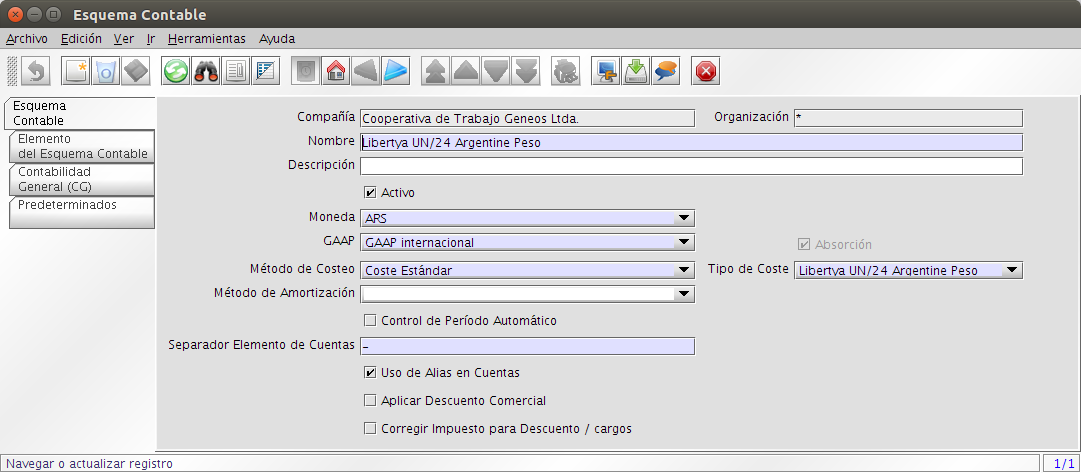
\includegraphics{ly_contabilidad_40.png}
\caption{Imagen 40: Esquema Contable \(\rightarrow\) Datos Generales}\end{figure}


\subsection{Configuración de cuentas contables por defecto}
\label{contabilidad:configuracion-de-cuentas-contables-por-defecto}\begin{enumerate}
\item {} 
Acceder a la pestaña \textbf{Predeterminados}, el sistema presenta una ventana como lo muestra la Imagen 41.

\item {} 
En esta pestaña puede modificarse los valores que por defecto el sistema asigna en el alta de entidades.

\end{enumerate}
\begin{figure}[htbp]
\centering
\capstart

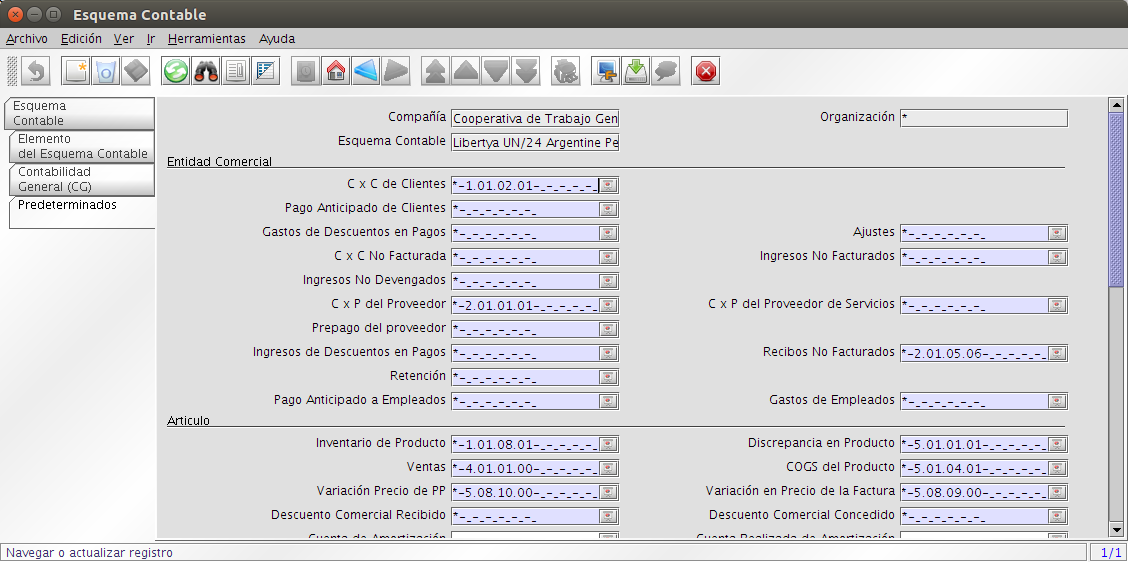
\includegraphics{ly_contabilidad_41.png}
\caption{Imagen 41: Esquema Contable \(\rightarrow\) Cuentas por Defecto}\end{figure}


\subsection{Elemento Contable}
\label{contabilidad:elemento-contable}
Permite la gestión del Plan de Cuentas de la organización.
\begin{enumerate}
\item {} 
Acceder con el perfil ``\textbf{Administración}'' a la opción del menú, \textbf{Contabilidad} \(\rightarrow\) \textbf{Elemento Contable}, el sistema presenta una ventana como lo muestra la Imagen 42.

\item {} 
Acceder a la pestaña Valor del Elemento, , el sistema presenta una ventana como lo muestra la Imagen 43. Despliega en forma de árbol el plan de cuentas, permitiendo su gestión, modificando elementos, agregando y reubicando en el árbol y eliminando.

\end{enumerate}
\begin{figure}[htbp]
\centering
\capstart

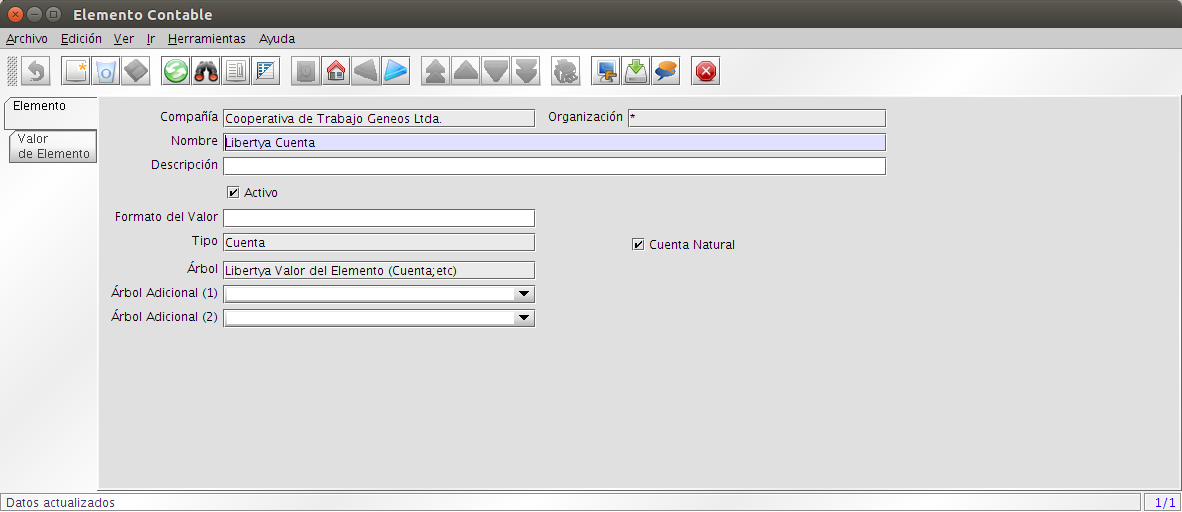
\includegraphics{ly_contabilidad_42.png}
\caption{Imagen 42: Elemento Contable \(\rightarrow\) Datos Generales}\end{figure}
\begin{figure}[htbp]
\centering
\capstart

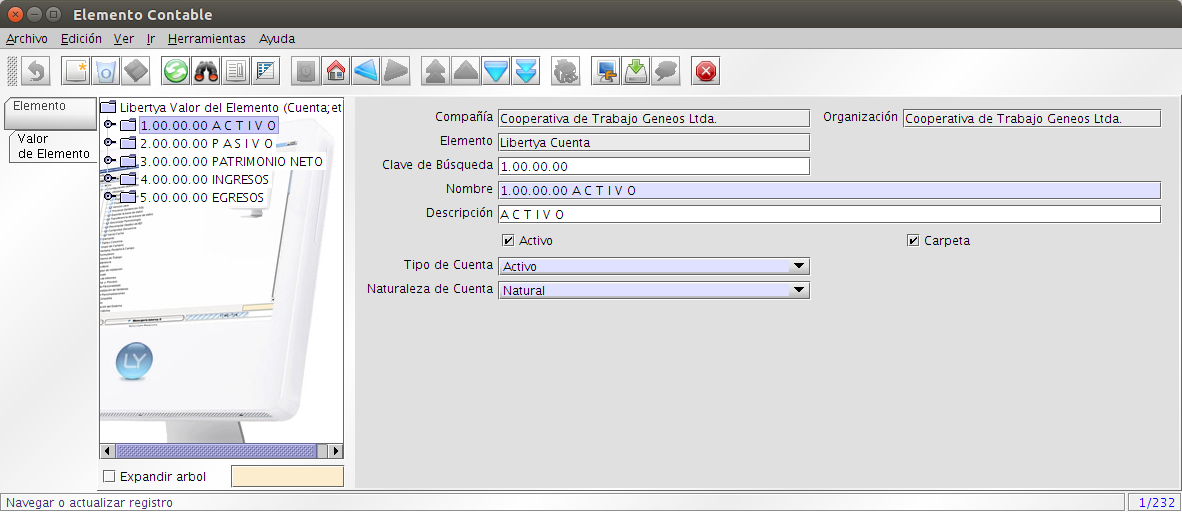
\includegraphics{ly_contabilidad_43.png}
\caption{Imagen 43: Elemento Contable \(\rightarrow\) Cuentas Contables}\end{figure}

\textbf{Nota}: es necesario respetar las convenciones de nomenclatura de las cuentas contables a la vez que su correcto agrupamiento en el árbol.

\textbf{Modificación de Cuentas Contables por defecto en registros}

Para cualquier ítem se debe seguir el mismo procedimiento:
\begin{enumerate}
\item {} 
Acceder a la pestaña Contabilidad del registro. En nuestro ejemplo de la Cuenta de un Banco, el sistema presenta una ventana como lo muestra la Imagen 44.

\item {} 
Seleccionar la Organización.

\item {} 
Seleccionar en el campo Cuenta, la cuenta a cambiar.

\item {} 
Guardar los cambios.

\item {} 
Confirmar la operación presionando el botón verde.

\end{enumerate}
\begin{figure}[htbp]
\centering
\capstart

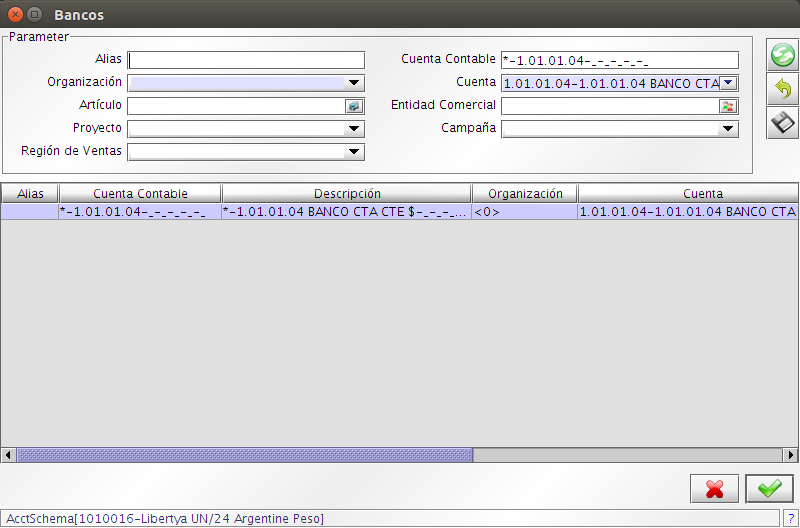
\includegraphics{ly_contabilidad_44.png}
\caption{Imagen 44: Cambio de Cuentas Contables}\end{figure}


\subsection{Asientos Manuales}
\label{contabilidad:asientos-manuales}\begin{enumerate}
\item {} 
Acceder con el perfil ``Administración'' a la opción del menú, Contabilidad \(\rightarrow\) Carga de Asientos Manuales, el sistema presenta una ventana como lo muestra la Imagen 45.

\item {} \begin{description}
\item[{\textbf{Lote},  el sistema presenta una ventana como lo muestra la Imagen 45:}] \leavevmode\begin{itemize}
\item {} 
Nro. de Documento, el sistema lo ingresa de forma automática en caso que no se especifique.

\item {} 
Descripción.

\item {} 
Tipo de Documento.

\item {} 
Fecha del Documento.

\item {} 
Fecha de Aplicación de CG.

\end{itemize}

\end{description}

\end{enumerate}

Completar, es la opción para procesar el asiento una vez cargados el Diario y Líneas.

3. \textbf{Diario},  el sistema presenta una ventana como lo muestra la Imagen 46.
Tipo de Documento.
Fecha del Documento.
Fecha de Aplicación de CG.
\begin{enumerate}
\setcounter{enumi}{3}
\item {} \begin{description}
\item[{\textbf{Línea},  el sistema presenta una ventana como lo muestra la Imagen 47.}] \leavevmode\begin{itemize}
\item {} 
Cuenta Contable

\item {} 
Descripción.

\item {} 
Debe.

\item {} 
Haber.

\end{itemize}

\end{description}

\end{enumerate}
\begin{figure}[htbp]
\centering
\capstart

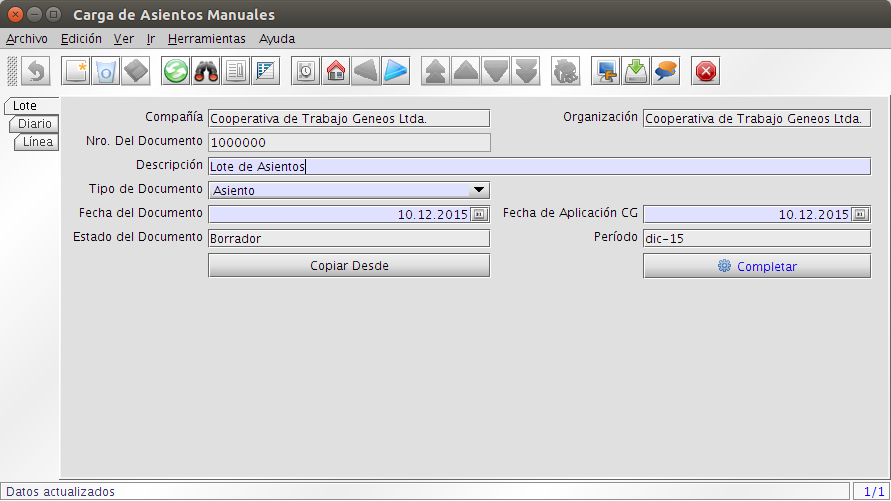
\includegraphics{ly_contabilidad_45.png}
\caption{Imagen 45: Carga de Asientos Manuales - Lote}\end{figure}
\begin{figure}[htbp]
\centering
\capstart

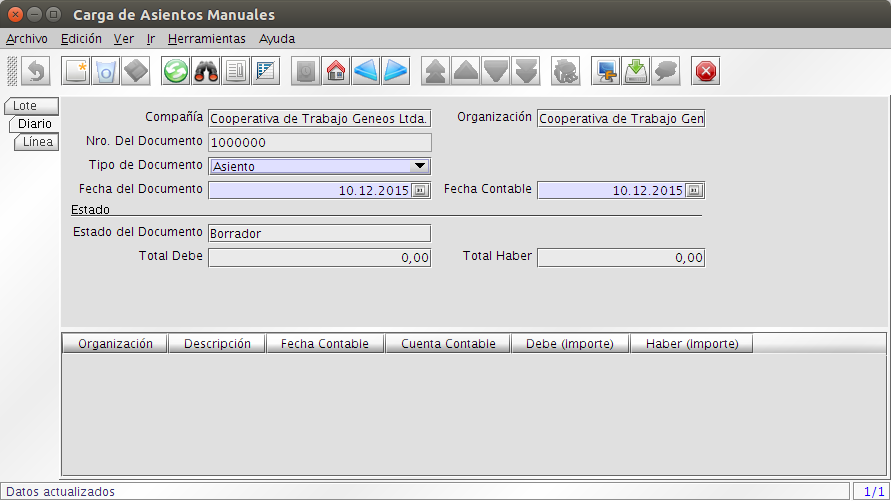
\includegraphics{ly_contabilidad_46.png}
\caption{Imagen 46: Carga de Asientos Manuales - Diario}\end{figure}
\begin{figure}[htbp]
\centering
\capstart

\includegraphics{ly_contabilidad_47.png}
\caption{Imagen 47: Carga de Asientos Manuales - Línea}\end{figure}


\chapter{Módulo de Stock}
\label{stock:modulo-de-stock}\label{stock::doc}
\textbf{Datos previos necesarios}
\begin{enumerate}
\item {} 
Almacenes y Ubicaciones

\item {} 
Artículos

\item {} 
Conjunto de Atributos (Opcional)

\item {} 
Cargos

\end{enumerate}


\section{Proceso de gestión de stock}
\label{stock:proceso-de-gestion-de-stock}\begin{enumerate}
\item {} \begin{description}
\item[{Ingresos de Artículos al Stock}] \leavevmode\begin{enumerate}
\item {} 
Ingresos por \textbf{Remito de Compras} (Ver módulo de Compras).

\item {} 
Ingresos por ajuste de \textbf{Inventario Físico}.

\item {} 
Ingresos por \textbf{Remito de Devolución de Clientes} (Ver módulo de Ventas).

\item {} 
Ingresos por \textbf{Devolución de Materiales para Producción}  (Ver módulo de Producción).

\item {} 
Cambio de Artículo.

\end{enumerate}

\end{description}

\item {} \begin{description}
\item[{Movimientos de Stock entre Almacenes}] \leavevmode\begin{enumerate}
\item {} 
\textbf{Movimiento de Inventario}.

\item {} \begin{description}
\item[{\textbf{Transferencia de Mercadería}.}] \leavevmode\begin{enumerate}
\item {} 
\textbf{Transferencia en dos Etapas}.

\item {} 
\textbf{Movimiento en dos Etapas}. Por ejemplo para envíos a garantía.

\end{enumerate}

\end{description}

\item {} 
\textbf{Entradas y Salidas Simples}. Por ejemplo para pérdidas.

\end{enumerate}

\end{description}

\item {} \begin{description}
\item[{Bajas de Stock}] \leavevmode\begin{enumerate}
\item {} 
Baja por ajuste de \textbf{Inventario Físico}.

\item {} 
Baja por \textbf{Entrega de Materiales para Producción} (Ver módulo de Producción).

\item {} 
Baja lógica por Movimientos de Inventario a almacenes de descarte.

\item {} 
Baja por \textbf{Remito de Entrega a Clientes} (Ver módulo de Compras).

\item {} 
Baja por \textbf{Remito de Devolución a Proveedores} (Ver módulo de Ventas).

\item {} 
Cambio de Artículo.

\end{enumerate}

\end{description}

\end{enumerate}


\section{Almacenes y Ubicaciones}
\label{stock:almacenes-y-ubicaciones}
Para poder almacenar artículos y tenerlos disponibles como stock, primero se han de definir una serie de Almacenes o Ubicaciones donde se almacenaran dichos productos.

\textbf{Almacén}

Para esto se utiliza la ventana de Almacén. En la pestaña principal se introduce un nombre y una dirección física para nuestro almacén, a fin de que dicha dirección pueda constar en los documentos que se generen. Este último dato es obligatorio.
\begin{enumerate}
\item {} 
Acceder a la opción de menú \textbf{Entidades Configuración de la Compañía \(\rightarrow\) Almacén y Ubicaciones}, por defecto ingresa a la primera pestaña de \textbf{Almacén}, el sistema presenta una ventana como lo muestra la Imagen 22.

\item {} \begin{description}
\item[{Campos a ingresar:}] \leavevmode\begin{itemize}
\item {} 
Compañía

\item {} 
Organización

\item {} 
Clave de Búsqueda

\item {} 
Nombre

\item {} 
Descripción

\item {} 
Activo

\item {} 
Localización / Dirección

\item {} 
Cargo de Fraccionamiento

\item {} 
Cargo de Merma

\item {} 
Cargo x Cambio de Artículo

\end{itemize}

\end{description}

\end{enumerate}
\begin{figure}[htbp]
\centering
\capstart

\includegraphics{ly_alm1.png}
\caption{Imagen 22: Almacenes}\end{figure}

\textbf{Ubicación}

En la siguiente pestaña se define cada una de las ubicaciones de las que costara el almacén.

Una ubicación es una combinación de un pasillo, una estantería y un nivel de profundidad. Esto permite definir todas las combinaciones de almacenamiento posibles. Adicionalmente, se puede definir una prioridad para que los artículos salgan primero de una determinada ubicación.
\begin{enumerate}
\item {} 
Acceder a la pestaña \textbf{Ubicación}, el sistema presenta una ventana como lo muestra la Imagen 23.

\item {} \begin{description}
\item[{Campos a ingresar:}] \leavevmode\begin{itemize}
\item {} 
Compañía

\item {} 
Organización

\item {} 
Almacén

\item {} 
Clave de Búsqueda

\item {} 
Activo

\item {} 
Prioridad Relativa

\item {} 
Predeterminado

\item {} 
Pasillo (X)

\item {} 
Estanteria (Y)

\item {} 
Nivel (Z)

\end{itemize}

\end{description}

\end{enumerate}
\begin{figure}[htbp]
\centering
\capstart

\includegraphics{ly_alm2.png}
\caption{Imagen 23: Ubicaciones}\end{figure}

\textbf{Almacenamiento}

En la tercera pestaña se podrá consultar a posteriori que artículos ha sido  asignados a la ubicación que se hubieran seleccionado en la pestaña anterior.
\begin{enumerate}
\item {} 
Acceder a la pestaña \textbf{Almacenamiento}, el sistema presenta una ventana como lo muestra la Imagen 24.

\item {} \begin{description}
\item[{Campos que informa la pestaña:}] \leavevmode\begin{itemize}
\item {} 
Compañía

\item {} 
Organización

\item {} 
Ubicación

\item {} 
Artículo

\item {} 
Instancia del Conjunto de Attributos

\item {} 
Activo

\item {} 
Stock

\item {} 
Ultima Fecha de Recuento de Inventarios

\item {} \begin{enumerate}
\setcounter{enumi}{15}
\item {} 
Servir

\end{enumerate}

\item {} \begin{enumerate}
\setcounter{enumi}{15}
\item {} 
Recibir

\end{enumerate}

\end{itemize}

\end{description}

\end{enumerate}
\begin{figure}[htbp]
\centering
\capstart

\includegraphics{ly_alm3.png}
\caption{Imagen 24: Almacenamiento}\end{figure}


\section{Cargos}
\label{stock:cargos}
Para algunas de las operaciones con Stock, se deben configurar elementos especiales, para detallar motivos y/o hacer afectación contable. Para esto se utilizan los \textbf{Cargos}.
\begin{enumerate}
\item {} 
Acceder a la opción de menú \textbf{Contabilidad \(\rightarrow\) Configuración de Contabilidad \(\rightarrow\) Cargo}, por defecto ingresa a la primera pestaña de \textbf{Almacén}, el sistema presenta una ventana como lo muestra la Imagen 25.

\item {} \begin{description}
\item[{Campos que informa la pestaña:}] \leavevmode\begin{itemize}
\item {} 
Compañía

\item {} 
Organización

\item {} 
Clave de Búsqueda

\item {} 
Nombre

\item {} 
Descripción

\item {} 
Activo

\item {} 
Tipo de Cargo

\item {} 
Signo

\item {} 
Importe de Cargo

\item {} 
Categoría del Impuesto

\item {} 
Impuesto Incluido en el Precio

\item {} 
Mismo Impuesto

\end{itemize}

\end{description}

\item {} 
Acceder a la pestaña \textbf{Contabilidad}, el sistema presenta una ventana como lo muestra la Imagen 26.

\item {} \begin{description}
\item[{Campos que informa la pestaña:}] \leavevmode\begin{itemize}
\item {} 
Compañía

\item {} 
Organización

\item {} 
Cargo

\item {} 
Esquema Contable

\item {} 
Activo

\item {} 
Cuenta de Otros Gastos

\item {} 
Cuenta de Otros Ingresos

\end{itemize}

\end{description}

\end{enumerate}
\begin{figure}[htbp]
\centering
\capstart

\includegraphics{ly_cargo.png}
\caption{Imagen 25: Cargo}\end{figure}
\begin{figure}[htbp]
\centering
\capstart

\includegraphics{ly_cargo_cont.png}
\caption{Imagen 26: Contabilidad de Cargo}\end{figure}


\section{Inventario Físico}
\label{stock:inventario-fisico}
Esta ventana se utiliza para realizar ajustes manuales al Stock.
\begin{enumerate}
\item {} 
Acceder a la opción de menú \textbf{Almacén \(\rightarrow\) Inventario Físico}, por defecto ingresa a la primera pestaña de \textbf{Recuento de Inventario}, el sistema presenta una ventana como lo muestra la Imagen 27.

\item {} \begin{description}
\item[{Campos que informa la pestaña:}] \leavevmode\begin{itemize}
\item {} 
Compañía

\item {} 
Organización

\item {} 
Nro. Del Documento

\item {} 
Descripción

\item {} 
Tipo de Documento

\item {} 
Fecha de Movimiento

\item {} 
Almacén

\item {} 
Configuracion de Inventario

\item {} 
Generar Lista

\item {} 
Actualizar Cantidades

\item {} 
Proyecto

\item {} 
Campaña

\item {} 
Aprobación

\item {} 
Cantidad Aprobada

\item {} 
Estado del Documento

\item {} 
Acción en el Documento

\end{itemize}

\end{description}

\item {} 
Acceder a la pestaña \textbf{Línea de Recuento de Inventario}, el sistema presenta una ventana como lo muestra la Imagen 28.

\item {} \begin{description}
\item[{Campos que informa la pestaña:}] \leavevmode\begin{itemize}
\item {} 
Compañía

\item {} 
Organización

\item {} 
Inventario Físico

\item {} 
Nro. Línea

\item {} 
Descripción

\item {} 
Artículo

\item {} 
Ubicación

\item {} 
Cantidad Contada

\item {} 
Cantidad según el sistema

\item {} 
Diferencia

\item {} 
Tipo de Inventario

\item {} 
Cargo (en caso que el Tipo de Inventario sea Cargo en Cuenta)

\end{itemize}

\end{description}

\end{enumerate}
\begin{figure}[htbp]
\centering
\capstart

\includegraphics{ly_invfisico_1.png}
\caption{Imagen 27: Inventario Físico}\end{figure}
\begin{figure}[htbp]
\centering
\capstart

\includegraphics{ly_invfisico_2.png}
\caption{Imagen 28: Inventario Físico - Líneas}\end{figure}


\section{Movimientos de Inventario}
\label{stock:movimientos-de-inventario}
Esta ventana se utiliza para realizar transferencias entre almacenes.
\begin{enumerate}
\item {} 
Acceder a la opción de menú \textbf{Almacén \(\rightarrow\) Movimiento de Inventario}, por defecto ingresa a la primera pestaña de \textbf{Movimiento}, el sistema presenta una ventana como lo muestra la Imagen 29.

\item {} \begin{description}
\item[{Campos que informa la pestaña:}] \leavevmode\begin{itemize}
\item {} 
Compañía

\item {} 
Organización

\item {} 
Nro. Del Documento

\item {} 
Descripción

\item {} 
Fecha de Movimiento

\item {} 
Tipo de Documento

\item {} 
Proyecto

\item {} 
Campaña

\item {} 
Aprobación

\item {} 
Cantidad Aprobada

\item {} 
En Tránsito

\item {} 
Fecha de Recibo

\item {} 
Estado del Documento

\item {} 
Acción en el Documento

\end{itemize}

\end{description}

\item {} 
Acceder a la pestaña \textbf{Línea de Movimiento}, el sistema presenta una ventana como lo muestra la Imagen 30.

\item {} \begin{description}
\item[{Campos que informa la pestaña:}] \leavevmode\begin{itemize}
\item {} 
Compañía

\item {} 
Organización

\item {} 
Movimiento

\item {} 
Nro. Línea

\item {} 
Descripción

\item {} 
Activo

\item {} 
Artículo

\item {} 
Conj. Atributos Origen

\item {} 
Conj. Atributos Destino

\item {} 
Ubicación

\item {} 
A Ubicación

\item {} 
Cantidad del Movimiento

\item {} 
Cantidad Destino

\item {} 
Cantidad Desechada

\item {} 
Cantidad Confirmada

\end{itemize}

\end{description}

\end{enumerate}
\begin{figure}[htbp]
\centering
\capstart

\includegraphics{ly_mov_1.png}
\caption{Imagen 29: Movimiento de Inventario}\end{figure}
\begin{figure}[htbp]
\centering
\capstart

\includegraphics{ly_mov_2.png}
\caption{Imagen 30: Movimiento de Inventario - Líneas}\end{figure}

\textbf{Transferencia de Mercadería}

\textbf{Entradas y Salidas Simples}


\chapter{Módulo de Manufactura}
\label{manufactura:modulo-de-manufactura}\label{manufactura::doc}
El módulo de Manufactura se basa en MRP (Material Resource Planning).

El MRP, consiste esencialmente, en un cálculo de necesidades netas de los artículos
(productos terminados, productos intermedios, materias primas) introduciendo un factor nuevo, no considerado en los métodos tradicionales de gestión de stocks, que es el plazo de fabricación o plazo de entrega en la compra de cada uno de los artículos, lo que en definitiva conduce a modular a lo largo del tiempo las necesidades, ya que indica la oportunidad de fabricar (o aprovisionar) los componentes, con la  debida planificación respecto a su utilización en la fase siguiente de fabricación.

\textbf{Datos utilizados por el MRP}

Fuentes principales
\begin{enumerate}
\item {} 
Plan Maestro detallado de Producción, que nos dice que productos finales hay que fabricar y en que plazos de entrega.

\item {} 
Lista de Materiales, indica de que partes o componentes se forma cada unidad de los productos intermedios y terminados, permitiendo calcular las cantidades de cada componente necesarias para fabricarlos.

\item {} 
Estado del Stock, permite conocer las cantidades disponibles de cada artículo y por diferencia, las cantidades que deben comprarse.

\end{enumerate}

Fuentes complementarias
\begin{enumerate}
\item {} 
Órdenes de Producción en curso, deben considerarse como futuras disponibilidades de producto, siempre y cuando las fechas de finalización de las órdenes coincidan con los plazos en los que se requieren los productos.

\item {} 
Órdenes de Compra en curso, deben considerarse como futuras disponibilidades de producto, siempre y cuando las fechas de entrega de las órdenes coincidan con los plazos en los que se requieren los productos.

\end{enumerate}

\textbf{Síntesis del Proceso MRP}
\begin{figure}[htbp]
\centering
\capstart

\includegraphics{ly_mrp.png}
\caption{Imagen 31: Síntesis MRP}\end{figure}

Contenidos:


\section{Manufactura - Flujos de Trabajo}
\label{manufactura-flujos:manufactura-flujos-de-trabajo}\label{manufactura-flujos::doc}
Los Flujos de Trabajo de Manufactura, definen la estructura de \textbf{Etapas productivas} y \textbf{Recursos} asociados a cada etapa.


\subsection{Tipos de Recursos de Manufactura}
\label{manufactura-flujos:tipos-de-recursos-de-manufactura}
Los \textbf{Tipo de Recurso de Manufactura} proveen un agrupamiento mediante una relación jerárquica: por ejemplo un \textbf{Centro de Trabajo} se puede integrar en una \textbf{Estación de Trabajo}, una \textbf{Línea de Producción}, que a su vez junto a otras líneas se integran en una \textbf{Planta}. Esta agrupación de tipos de recursos, se utilizará para calcular la capacidad requerida y disponible de producción mediante la sumatoria individual de las capacidades de cada recurso.

Un primer nivel de agrupamiento será utilizado para definir una tipología de recursos que tengan en común una serie de características.
\begin{enumerate}
\item {} 
Acceder a la opción del menú \textbf{Gestión de Ingeniería \(\rightarrow\)  Recursos de Manufactura \(\rightarrow\) Tipo de Recurso de Manufactura}. El sistema presenta una ventana como lo muestra la Imagen 32.

\item {} \begin{description}
\item[{Campos a ingresar:}] \leavevmode\begin{itemize}
\item {} 
\textbf{Compañía:} Cliente para esta instalación Compañía o entidad legal

\item {} 
\textbf{Organización:} Entidad organizacional dentro de la compañía.

\item {} 
\textbf{Clave de Búsqueda} Clave de búsqueda para el registro en el formato requerido; debe ser única.

\item {} 
\textbf{Nombre:} Identificador alfanumérico de la entidad. El nombre de una entidad (registro) se usa como una opción de búsqueda predeterminada adicional a la clave de búsqueda. El nombre es de hasta 60 caracteres de longitud.

\item {} 
\textbf{Descripción:} Descripción corta opcional del registro Una descripción esta limitada a 255 caracteres.

\item {} 
\textbf{Activo:} El registro está activo en el sistema Hay dos métodos para que los registros no estén disponibles en el sistema: Uno es eliminar el registro; el otro es desactivarlo. Un registro desactivado no está disponible para selección; pero está disponible para Informes.

\item {} 
\textbf{UM:} Unidad de Medida La UM define una unidad de medida única (dias, horas, kilos, litros).

\item {} 
\textbf{Permitir fracciones de UM:} Permitir fracciones de unidad de medida Si se habilita; se puede entrar fracciones de la unidad de medida.

\item {} 
\textbf{Asignación Única solamente:} Solamente una asignación a la vez (No se puede tener asignaciones dobles de tiempo o asignaciones concurrentes) Si se selecciona; solo se puede tener una asignación a la vez para un momento en el tiempo. No es posible tener asignaciones concurrentes.

\item {} 
\textbf{Tiempo Disponible:} Indica si el recurso está disponible sólo en algún momento, habilita los campos Inicio y Final.

\item {} 
\textbf{Inicio:} Momento cuando el tiempo disponible comienza.

\item {} 
\textbf{Final:} Momento cuando el tiempo disponible finaliza.

\item {} 
\textbf{Día Disponible:} Indica si el recurso está disponible sólo algunos días de la semana, habilita los campos para cada uno de los días (lunes, martes, miércoles, jueves, viernes, sábado y domingo).

\end{itemize}

\end{description}

\item {} 
Guardar.

\end{enumerate}
\begin{figure}[htbp]
\centering
\capstart

\includegraphics{ly_tiporecurso.png}
\caption{Imagen 32: Tipo de Recurso de Manufactura}\end{figure}


\subsection{Recurso de manufactura}
\label{manufactura-flujos:recurso-de-manufactura}
Ahora podemos definir todos los Recursos de Manufactura, clasificados mediante los Tipos de Recursos, para poder utilizarlos luego en el Flujo de Trabajo.

Un \textbf{Recurso de Manufactura} es cualquier cosa requerida como soporte para el proceso de producción. Principalmente responde a la pregunta: ¿En dónde se hace un producto?. Cada recurso de trabajo es único dentro de la organización y puedo definir tantos recursos como sea necesario.
\begin{enumerate}
\item {} 
Acceder a la opción del menú \textbf{Gestión de Ingeniería \(\rightarrow\)  Recursos de Manufactura \(\rightarrow\) Recurso de Manufactura}. El sistema presenta una ventana como lo muestra la Imagen 33.

\item {} \begin{description}
\item[{Campos a ingresar:}] \leavevmode\begin{itemize}
\item {} 
\textbf{Compañía:} Cliente para esta instalación Compañía o entidad legal

\item {} 
\textbf{Organización:} Entidad organizacional dentro de la compañía.

\item {} 
{\color{red}\bfseries{}**}Tipo de Recurso: ** Es el Tipo de Recurso de Manufactura registrado en el paso anterior.

\item {} 
\textbf{Clave de Búsqueda} Clave de búsqueda para el registro en el formato requerido; debe ser única.

\item {} 
\textbf{Nombre:} Identificador alfanumérico de la entidad. El nombre de una entidad (registro) se usa como una opción de búsqueda predeterminada adicional a la clave de búsqueda. El nombre es de hasta 60 caracteres de longitud.

\item {} 
\textbf{Descripción:} Descripción corta opcional del registro Una descripción esta limitada a 255 caracteres.

\item {} 
\textbf{Activo:} El registro está activo en el sistema Hay dos métodos para que los registros no estén disponibles en el sistema: Uno es eliminar el registro; el otro es desactivarlo. Un registro desactivado no está disponible para selección; pero está disponible para Informes.

\item {} 
\textbf{Almacén:} El Almacén indica un Almacén único donde los productos son almacenados.

\item {} 
\textbf{Usuario:} Indica un usuario de referencia o contacto.

\item {} 
\textbf{Disponible:} Indica si el recurso está disponible.

\item {} 
\textbf{Es Recurso Manufactura:} Indica si el recurso es requerido para la producción. Este campo debe estar seleccionado.

\item {} 
\textbf{Tipo de Recurso Manufactura:} Es el Tipo de Recurso Manufactura General, al menos uno de los Recursos debe ser del tipo \textbf{Planta} y deberá configurarse en el Flujo de Trabajo de Manufactura.

\item {} 
\textbf{Tiempo Encolado:} Es una referencia donde se ingresa el tiempo total de encolado del recurso.

\item {} 
\textbf{Tiempo de espera:} El tiempo de preparación es el requerido para ejecutar las actividades necesarias para preparar el recurso de manufactura hasta que esté listo para comenzar con el proceso de fabricación.

\end{itemize}

\end{description}

\item {} 
Guardar.

\end{enumerate}
\begin{figure}[htbp]
\centering
\capstart

\includegraphics{ly_recurso.png}
\caption{Imagen 33: Recurso de Manufactura}\end{figure}


\section{Manufactura - Lista de Materiales}
\label{manufactura-bom:manufactura-lista-de-materiales}\label{manufactura-bom::doc}
Permite definir la composición de los productos fabricados, tanto intermedios como  terminados. Se pueden tener distintos niveles intermedios de producción, los  niveles intermedios definen la fabricación de productos que serán entrada de otros procesos productivos de niveles superiores.


\subsection{Lista de materiales y fórmulas}
\label{manufactura-bom:lista-de-materiales-y-formulas}\begin{enumerate}
\item {} 
Acceder a la opción de menú \textbf{Gestión de Manufactura \(\rightarrow\) Gestión de Ingeniería \(\rightarrow\) Lista de Materiales y Fórmulas \(\rightarrow\) Lista de Materiales y Fórmula}. El sistema presenta una ventana como lo muestra la Imagen 34.

\item {} \begin{description}
\item[{Campos a ingresar en la cabecera:}] \leavevmode\begin{itemize}
\item {} 
\textbf{Compañía:} Cliente para esta instalación compañía o entidad legal

\item {} 
\textbf{Organización:} Entidad organizacional dentro de la compañía. Una organización es una unidad de la compañía o entidad legal.

\item {} 
Producto:** Producto que va a tener una fórmula asociada.

\item {} 
\textbf{UM:} Unidad de Medida se refiere a unidades de medida no monetarias y además define si se permite la conversión entre unidades de medida y cómo se van a calcular.

\item {} 
\textbf{Nombre:} Identificador alfanumérico de la entidad. El nombre de una entidad (registro) se usa como una opción de búsqueda predeterminada adicional a la clave de búsqueda. El nombre es de hasta 60 caracteres de longitud.

\item {} 
\textbf{Descripción:} Descripción corta opcional del registro Una descripción esta limitada a 255 caracteres.

\item {} 
\textbf{Ayuda:} El campo Ayuda contiene una sustento, comentario o ayuda acerca de cómo usar este ítem.

\item {} 
\textbf{Activo:} El registro está activo en el sistema Hay dos métodos para que los registros no estén disponibles en el sistema: Uno es eliminar el registro; el otro es desactivarlo. Un registro desactivado no está disponible para selección; pero está disponible para Informes

\item {} 
\textbf{Aviso de Cambio:} Cuenta de materiales (ingeniería) cambio de aviso (versión).

\item {} 
\textbf{Nro del Documento:} Número de secuencia del documento para cada documento creado. El número del documento es usualmente generado en automático por el sistema y determinado por el tipo del documento. Si el documento no se salva; el número preliminar se despliega entre ``\textless{}\textgreater{}''.

\item {} 
\textbf{Tipo LDM:} Tipo de Lista de Materiales.

\item {} 
\textbf{LDM Usada:} Uso de lista de materiales. El predeterminado de la LDM es usado, Si hay alternativos no están definidos.

\end{itemize}

\end{description}

\item {} 
Guardar.

\item {} 
Seleccionar la pestaña \textbf{Componentes de la LDM \& Fórmula}, el sistema presenta una ventana como lo muestra la Imagen 35.

\item {} \begin{description}
\item[{Campos a ingresar:}] \leavevmode\begin{itemize}
\item {} 
\textbf{Compañía:} Cliente para esta instalación compañía o entidad legal

\item {} 
\textbf{Organización:} Entidad organizacional dentro de la compañía. Una organización es una unidad de la compañía o entidad legal.

\item {} 
\textbf{No. Línea:} Indica el Número de Línea único y controlará el orden de despliegue de las líneas dentro de un documento. Lo define el sistema de forma automática.

\item {} 
\textbf{Artículo:} Identifica un elemento/producto que es parte de una lista de materiales.

\item {} \begin{description}
\item[{\textbf{Tipo de componente:}}] \leavevmode\begin{itemize}
\item {} 
Componente: identifica a una materia prima, ingrediente, parte o subproducto que es utilizado en el ensamblado de un proceso de fabricación superior.

\item {} 
Co producto: esta entidad no es un producto programado obtenido como consecuencia de otro proceso de producción.

\item {} 
Empaque: este producto no será tenido en cuenta para calcular la cantidad total de componentes cuando la opción “Es Porcentaje Cantidad” se encuentre seleccionado.

\item {} 
Fantasma: indica que el producto es un ensamble ficticio, esto es, un conjunto de componentes que se agrupan sólo para hacer más fácil el análisis de forma separada del resto de la LDM. Cuando el MRP genera un requerimiento del fantasma y lo proyectado no está disponible, el proceso va al nivel mínimo y comienza un nuevo ciclo de MRP pero sin crear órdenes del producto fantasma.

\item {} 
Nota: Define el comportamiento del producto en la fórmula.

\end{itemize}

\end{description}

\end{itemize}

\end{description}

\item {} 
Guardar.

\end{enumerate}
\begin{figure}[htbp]
\centering
\capstart

\includegraphics{ly_ldm_1.png}
\caption{Imagen 34: Lista de Materiales}\end{figure}
\begin{figure}[htbp]
\centering
\capstart

\includegraphics{ly_ldm_2.png}
\caption{Imagen 35: Lista de Materiales - Componentes}\end{figure}


\section{Manufactura - Datos de Planificación de producto}
\label{manufactura-plan:manufactura-datos-de-planificacion-de-producto}\label{manufactura-plan::doc}
Para calcular el Plan de Materiales, primero debemos configurar los \textbf{Datos de Planeamiento de los Productos} que intervienen en el proceso productivo.

Los Datos de Planeamiento de los Productos varían según los productos sean comprados o fabricados. Para los primeros se deben configurar los datos relacionados a tiempos y políticas de compra, mientras que para los segundos, los datos y políticas de fabricación, entre ellos la Lista de Materiales y el Flujo de Trabajo.
\begin{enumerate}
\item {} 
Acceder a la opción del menú \textbf{Gestión de Manufactura \(\rightarrow\)  Gestión de Planificación \(\rightarrow\) Datos de Planificación de Productos}. El sistema presenta una ventana como lo muestra la Imagen 36. Buscar el producto a configurar en la primera pestaña.

\item {} 
Acceder a la pestaña \textbf{Línea de Movimiento}, el sistema presenta una ventana como lo muestra la Imagen 37.

\item {} \begin{description}
\item[{Campos a ingresar:}] \leavevmode\begin{itemize}
\item {} 
\textbf{Compañía:} Cliente para esta instalación compañía o entidad legal

\item {} 
\textbf{Organización:} Entidad organizacional dentro de la compañía. Una organización es una unidad de la compañía o entidad legal.

\item {} 
\textbf{Activo:} El registro está activo en el sistema Hay dos métodos para que los registros no estén disponibles en el sistema: Uno es eliminar el registro; el otro es desactivarlo. Un registro desactivado no está disponible para selección; pero está disponible para Informes.

\item {} 
\textbf{Recurso:} Recurso de tipo Planta para esta configuración de Datos de Planeamiento.

\item {} 
\textbf{Almacén:} Almacén para esta configuración de Datos de Planeamiento.

\item {} 
\textbf{Planificador}

\item {} 
\textbf{Lista de Materiales:} En caso de productos fabricados, la Lista de Materiales correspondiente.

\item {} 
\textbf{Flujo de Trabajo:}  En caso de productos fabricados, el Flujo de Trabajo correspondiente.

\item {} 
\textbf{Crear Plan:} Si queremos que en la configuración de Datos de Planeamiento entre en consideración del MRP.

\item {} 
\textbf{Es MRP Requerido:} Lo pone el sistema de forma automática, si algún cambio en las configuraciones, requiere correr nuevamente el MRP.

\item {} \begin{description}
\item[{\textbf{Tiempos de Gestión:}}] \leavevmode\begin{itemize}
\item {} 
\textbf{Tiempo de Entrega Prometido}

\item {} 
\textbf{Protección Tiempo}

\item {} 
\textbf{Tiempo de Trabajo}

\item {} 
\textbf{Tiempo de Transferencia}

\end{itemize}

\end{description}

\item {} 
\textbf{Política de Ordenamiento:}

\item {} 
\textbf{Periodo de Pedido:}

\item {} 
\textbf{Cantidad del Pedido:}

\item {} 
\textbf{Múltiplo a Ordenar:}

\item {} 
\textbf{Cantidad Mínima de Pedido:}

\item {} 
\textbf{Cantidad Máxima del Pedido:}

\item {} 
\textbf{\% Rendimiento:}

\item {} 
\textbf{Cantidad Existencia Seguridad:}

\item {} 
\textbf{Es alternativo:}

\end{itemize}

\end{description}

\item {} 
Guardar.

\end{enumerate}
\begin{figure}[htbp]
\centering
\capstart

\includegraphics{ly_planeam_1.png}
\caption{Imagen 36: Planeamiento}\end{figure}
\begin{figure}[htbp]
\centering
\capstart

\includegraphics{ly_planeam_2.png}
\caption{Imagen 37: Planeamiento - Datos de Planeamiento}\end{figure}


\section{Manufactura - Pronóstico}
\label{manufactura-pronostico:manufactura-pronostico}\label{manufactura-pronostico::doc}
El Pronóstico permite definir la proyección de la producción que va a tener como entrada el proceso del MRP. Los elementos del pronóstico definen fechas y cantidades necesarias, para cada producto, generalmente a nivel de productos finales, lo que no quita que puedan agregarse pronósticos de productos intermedios. El pronóstico puede tener, una o varias de las siguientes entradas:
\begin{itemize}
\item {} 
Producción por ventas planificadas

\item {} 
Producción por ventas regulares

\item {} 
Producción por ventas estacionales

\item {} 
Producción por aprovisionamiento

\item {} 
Otras

\end{itemize}
\begin{enumerate}
\item {} 
Acceder a la opción del menú \textbf{Gestión de Manufactura \(\rightarrow\)  Gestión de Planificación \(\rightarrow\) Provisión/Pronóstico de Materiales}. El sistema presenta una ventana como lo muestra la Imagen 38.

\item {} \begin{description}
\item[{Campos a ingresar en la cabecera:}] \leavevmode\begin{itemize}
\item {} 
\textbf{Compañía:} Cliente para esta instalación compañía o entidad legal

\item {} 
\textbf{Organización:} Entidad organizacional dentro de la compañía. Una organización es una unidad de la compañía o entidad legal.

\item {} 
\textbf{Nombre:} Identificador alfanumérico de la entidad. El nombre de una entidad (registro) se usa como una opción de búsqueda predeterminada adicional a la clave de búsqueda. El nombre es de hasta 60 caracteres de longitud.

\item {} 
\textbf{Descripción:} Descripción corta opcional del registro Una descripción esta limitada a 255 caracteres.

\item {} 
\textbf{Ayuda:} El campo Ayuda contiene una sustento, comentario o ayuda acerca de cómo usar este ítem.

\item {} 
\textbf{Activo:} El registro está activo en el sistema Hay dos métodos para que los registros no estén disponibles en el sistema: Uno es eliminar el registro; el otro es desactivarlo. Un registro desactivado no está disponible para selección; pero está disponible para Informes.

\item {} 
\textbf{Predeterminado:} Indica si el pronóstico es el predeterminado para la corrida del proceso de MRP.

\item {} 
\textbf{Calendario}.

\item {} 
\textbf{Año}.

\end{itemize}

\end{description}

\item {} 
Guardar.

\item {} 
Seleccionar pestaña \textbf{Línea}, el sistema presenta una ventana como lo muestra la Imagen 39.

\item {} \begin{description}
\item[{Campos a ingresar:}] \leavevmode\begin{itemize}
\item {} 
\textbf{Compañía:} Cliente para esta instalación compañía o entidad legal

\item {} 
\textbf{Organización:} Entidad organizacional dentro de la compañía. Una organización es una unidad de la compañía o entidad legal.

\item {} 
\textbf{Comercial/Usuario:} Responsable del registro de pronóstico.

\item {} 
\textbf{Recurso:} Recurso de tipo Planta donde va a ejecutarse el pronóstico.

\item {} 
\textbf{Almacén:} Almacén donde va a ejecutarse el pronóstico.

\item {} 
\textbf{Artículo:} Artículo pedido.

\item {} 
\textbf{UM:} Unidad de Medida asociada al artículo.

\item {} 
\textbf{Cantidad:} Cantidad pedida.

\item {} 
\textbf{Período:} Período del calendario y del año del pronóstico asociado al requerimiento.

\item {} 
\textbf{Fecha Prometida:} fecha para la cual es necesario el requerimiento.

\item {} 
\textbf{Activo:} El registro está activo en el sistema Hay dos métodos para que los registros no estén disponibles en el sistema: Uno es eliminar el registro; el otro es desactivarlo. Un registro desactivado no está disponible para selección; pero está disponible para Informes.

\end{itemize}

\end{description}

\item {} 
Guardar

\end{enumerate}
\begin{figure}[htbp]
\centering
\capstart

\includegraphics{ly_pronost_1.png}
\caption{Imagen 38: Pronóstico}\end{figure}
\begin{figure}[htbp]
\centering
\capstart

\includegraphics{ly_pronost_2.png}
\caption{Imagen 39: Pronóstico - Líneas}\end{figure}

La demanda de producción también puede generarse a través de órdenes de manufactura manuales.


\section{Manufactura - Checklist para correr el proceso de MRP}
\label{manufactura-checklist::doc}\label{manufactura-checklist:manufactura-checklist-para-correr-el-proceso-de-mrp}

\subsection{Consideraciones Generales}
\label{manufactura-checklist:consideraciones-generales}\begin{itemize}
\item {} 
Tanto el producto padre, como todos los componentes del mismo, tienen que tener Datos de Planificación de producto.

\item {} 
Al menos tenemos que tener un recurso de tipo Planta.

\item {} 
Establecer el horizonte de la planta en un valor \textgreater{} 0, tener en cuenta que esto valida las posibles demandas futuras, o sea si tengo una demanda más allá del horizonte no van a ser explotadas.

\item {} 
Tener un pronóstico / demanda para el período actual

\item {} 
Correr el proceso Verificar Lista de Materiales para cada familia

\end{itemize}


\subsection{Si el componente es comprado}
\label{manufactura-checklist:si-el-componente-es-comprado}\begin{itemize}
\item {} 
En la ventana \textbf{Artículo}, pestaña \textbf{Artículo}, desmarcar el casilla de verificación \textbf{Es Manufacturado} y marcar el check \textbf{Comprado}.

\item {} 
En la ventana \textbf{Artículo}, pestaña \textbf{Compras}, cargar un registro con un proveedor asociado por defecto.

\item {} \begin{description}
\item[{En la ventana \textbf{Datos de Planificación del Producto}, pestaña \textbf{Datos de Planificación}, cargar datos que correspondan:}] \leavevmode\begin{itemize}
\item {} 
Recurso (la Planta donde se va a producir).

\item {} 
Almacén.

\item {} 
Política de Ordenamiento.

\item {} 
Tiempos (no es mandatorio, dependen de cada producto y de la Política de Ordenamiento).

\item {} 
Cantidades (no es mandatorio, dependen de cada producto y de la Política de Ordenamiento).

\item {} 
Marcar el check Crear Plan.

\end{itemize}

\end{description}

\end{itemize}


\subsection{Si el componente es fabricado}
\label{manufactura-checklist:si-el-componente-es-fabricado}\begin{itemize}
\item {} 
En la ventana \textbf{Artículo}, pestaña \textbf{Artículo}, marcar el casilla de verificación \textbf{Es Manufacturado} y desmarcar el casilla de verificación \textbf{Comprado}..

\item {} \begin{description}
\item[{En la ventana \textbf{Datos de Planificación del Producto}, pestaña \textbf{Datos de Planificación}, cargar datos que correspondan:}] \leavevmode\begin{itemize}
\item {} 
Recurso (la Planta donde se va a producir).

\item {} 
Almacén.

\item {} 
Lista de Materiales.

\item {} 
Flujo de Trabajo

\item {} 
Política de Ordenamiento.

\item {} 
Tiempos (no es mandatorio, dependen de cada producto y de la Política de Ordenamiento).

\item {} 
Cantidades (no es mandatorio, dependen de cada producto y de la Política de Ordenamiento).

\item {} 
Marcar el casilla de verificación Crear Plan.

\end{itemize}

\end{description}

\end{itemize}


\section{Manufactura - Ejecución del MRP}
\label{manufactura-proceso:manufactura-ejecucion-del-mrp}\label{manufactura-proceso::doc}
La ejecución del Proceso de MRP debe completarse siguiendo los paso detallados a continuación:


\subsection{Paso 1: Calcular Niveles Inferiores}
\label{manufactura-proceso:paso-1-calcular-niveles-inferiores}
Este proceso calcula y registra el nivel menor de un producto dentro de una LDM. Es usado en los cálculos del MRP y debe ser ejecutado cuando ingresa una nueva LDM.
\begin{enumerate}
\item {} 
Acceder a la opción de menú \textbf{Gestión de Manufactura \(\rightarrow\) Gestión de Planificación \(\rightarrow\) MRP \(\rightarrow\) Calcular Niveles Inferiores}. El sistema presenta una ventana como lo muestra la Imagen 40.

\item {} 
Ejecutar Proceso.

\end{enumerate}
\begin{figure}[htbp]
\centering
\capstart

\includegraphics{ly_mrp_niveles.png}
\caption{Imagen 40: Calcular Niveles Inferiores}\end{figure}


\subsection{Paso 2: Crear Registros MRP}
\label{manufactura-proceso:paso-2-crear-registros-mrp}
Este proceso recrea la demanda, órdenes aprobadas y abiertas para un producto.
\begin{enumerate}
\item {} 
Acceder a la opción de menú \textbf{Gestión de Manufactura \(\rightarrow\) Gestión de Planificación \(\rightarrow\) MRP \(\rightarrow\) Crear Registros MRP}. El sistema presenta una ventana como lo muestra la Imagen 41.

\item {} 
Ejecutar Proceso.

\end{enumerate}
\begin{figure}[htbp]
\centering
\capstart

\includegraphics{ly_mrp_registros.png}
\caption{Imagen 41: Crear Registros MRP}\end{figure}


\subsection{Paso 3: Calcular Plan de Materiales}
\label{manufactura-proceso:paso-3-calcular-plan-de-materiales}
Cumplidos los pasos anteriores, podemos calcular el plan de materiales.

Durante este proceso se establece si las existencias y las requisiciones existentes satisfacen las necesidades para la producción. Este proceso calcula la demanda, órdenes aprobadas y abiertas para un producto.

Cuando este proceso finaliza, se muestra un resumen de las Órdenes de Manufactura, los Avisos de Pedido a Proveedores y los Avisos del MRP que fueron generados.
\begin{enumerate}
\item {} 
Acceder a la opción de menú \textbf{Gestión de Manufactura \(\rightarrow\) Gestión de Planificación \(\rightarrow\) MRP \(\rightarrow\) Calcular Plan de Materiales}. El sistema presenta una ventana como lo muestra la Imagen 42.

\item {} 
Ejecutar Proceso.

\end{enumerate}
\begin{figure}[htbp]
\centering
\capstart

\includegraphics{ly_mrp_calcular.png}
\caption{Imagen 42: Calcular Plan de Materiales}\end{figure}


\subsection{Avisos del MRP}
\label{manufactura-proceso:avisos-del-mrp}
Contiene un grupo de mensajes generados por el proceso MRP. Indica al usuario que acciones son necesarias, para poder alcanzar el Planeamiento de Producción correctamente.
\begin{enumerate}
\item {} 
Acceder al botón \textbf{Aviso} de la pantalla principal de la aplicación (barra inferior a la izquierda). El sistema presenta una ventana como lo muestra la Imagen 43.

\end{enumerate}
\begin{figure}[htbp]
\centering
\capstart

\includegraphics{ly_avisos.png}
\caption{Imagen 43: Avisos}\end{figure}

\textbf{Referencias}


\section{Manufactura - Orden de Manufactura}
\label{manufactura-om:manufactura-orden-de-manufactura}\label{manufactura-om::doc}
\textless{}\textless{}\textless{}\textless{}\textless{}\textless{}\textless{} HEAD
Una Orden de Manufactura es un documento que indica a la planta el compromiso de
fabricar un producto en una cantidad establecida y en una fecha específica.
Para  generar  o  modificar  manualmente  una  Orden  de  Manufactura  debemos ir a:
Manufactura -\textgreater{} Control de Producción -\textgreater{} Manufactura Discreta -\textgreater{} Orden de Manufactura.

La Orden de Manufactura integra componentes de la lista de materiales, del flujo de
trabajo y de los datos de planeamiento.

\textbf{Fecha de última Entrega}:Es la fecha de la última vez que el material de esta orden
fue entregado al almacén.

\textbf{Fecha de Inicio programada}: Es la fecha en que el MRP establece que la orden
debe ser surtida a la planta.

\textbf{Fecha de Terminación Programada}: Es la fecha en que el MRP establece que la
orden debe ser entregada al almacén.

\textbf{Fecha de Inicio Real}: Es la fecha en que la orden es liberada a la planta para ser
producida.

\textbf{Fecha de Terminación Real}: Es la fecha en que se elabora el cierre de la orden.

\textbf{Flotación Anterior} – Se utilizará posteriormente para el proceso de balanceo de la
carga de Recursos.

\textbf{Flotación Posterior} – Se utilizará posteriormente para el balanceo de la carga de
Recursos.

En el \textbf{Grupo Cantidades} se introduce la cantidad de producto a fabricar con  la Orden de Manufactura y su Unidad de Medida.

La \textbf{Cantidad del Lote} y la \textbf{Cantidad del Tamaño del lote} nos indica cuantos lotes de producción integran la OM y de que tamaño serán. Estos datos son tomados del Flujo de Trabajo de la OM.

En el campo \textbf{Cantidad Entregada} se muestra la cantidad que ha sido entregada al almacén de producto terminado hasta el momento.

La \textbf{cantidad Rechazada}: en este campo se muestra la cantidad que no ha cubierto las  especificaciones  de  calidad  hasta  el  momento  y  que  por  lo  tanto  deberá  ser posteriormente  reprocesada  o  enviada  al  desperdicio,  en  éste  último  caso  esa cantidad se desplegará en el campo Desperdicio.

En  el  campo \textbf{Rendimiento} se  despliega  la  cantidad  de  producto  que  reúne  las especificaciones de calidad dividida entre la cantidad total de la orden a producir.


\subsection{\textbf{Proyecto y Campaña} se refieren a las dimensiones estándar de Libertya.}
\label{manufactura-om:proyecto-y-campana-se-refieren-a-las-dimensiones-estandar-de-libertya}
Una \textbf{Orden de Manufactura} es un documento que indica a la planta el compromiso de fabricar un producto en una cantidad establecida y en una fecha específica.

Si bien las Ordenes de anufactura sn generadas de formaq automática por el MRP, también pueden ser modificadas y/o creadas manualmente.
\begin{enumerate}
\item {} 
Acceder a la opción del menú \textbf{Gestión de Manufactura \(\rightarrow\)  Gestión de la Producción \(\rightarrow\) Orden de Manufactura}. El sistema presenta una ventana como lo muestra la Imagen 43.

\item {} \begin{description}
\item[{Campos a ingresar:}] \leavevmode\begin{itemize}
\item {} 
\textbf{Compañía:} Compañía o empresa que utiliza ésta instalación. Compañía, empresa o entidad legal. No se puede compartir datos entre compañías.

\item {} 
\textbf{Organización:} Entidad organizacional dentro de la compañía. Una organización es una unidad de la compañía o entidad legal - Ej. Tiendas y departamentos.

\item {} 
\textbf{Nro. Del Documento:} Número identificador de la Orden de Manufactura. Es usualmente generado automáticamente por el sistema y determinado por el tipo del documento.

\item {} 
\textbf{Tipo Documento Destino:} Debe ser Orden de Manufactura.

\item {} 
\textbf{Activo:} El registro está activo en el sistema. Hay dos métodos para que los registros no estén disponibles en el sistema: Uno es eliminar el registro; el otro es desactivarlo. Un registro desactivado no está disponible para selección; pero está disponible para reportes.

\item {} 
\textbf{Descripción:} Descripción corta opcional del registro. Una descripción esta limitada a 255 caracteres.

\item {} 
\textbf{Artículo:} Artículo objeto de la producción asociada a esta Orden de Manufactura.

\item {} 
\textbf{Lista de Materiales:} Lista de Materiales asociada al artículo objeto de la producción asociada a esta Orden de Manufactura.

\item {} 
\textbf{Recurso:} Planta donde se realiza la producción.

\item {} 
\textbf{Flujo de Trabajo:} Flujo de trabajo o combinación de tareas, asociado al artículo objeto de la producción asociada a esta Orden de Manufactura.

\item {} 
\textbf{Almacén:} Almacén asociado al artículo objeto de la producción asociada a esta Orden de Manufactura.

\item {} 
\textbf{Prioridad:} Prioridad de un documento. La prioridad indica la importancia (alta; media; baja) de este documento.

\item {} 
\textbf{Fecha de la Orden}

\item {} 
\textbf{Fecha Prometida:} Indica la fecha en la que se espera la Orden de Manufactura este finalizada. Indica la fechaen que la orden fue prometida al cliente.

\item {} 
\textbf{Fecha de Confirmación}

\item {} 
\textbf{Fecha de la Entrega}

\item {} 
\textbf{Fecha Inicio programada:} Fecha Inicio Programada para la OM.

\item {} 
\textbf{Fecha Final Programada:} Fecha Final Programada para la OM.

\item {} 
\textbf{Fecha de Inicio:} Es la fecha cuando el primer movimiento de la orden de manufactura fue reportado, este movimiento puede ser un inventario o movimiento de labor.

\item {} 
\textbf{Fecha de Terminación:} La fecha final se usa para indicar cuando se espera que el proyecto se complete o cuando ha sido completado.

\item {} 
{\color{red}\bfseries{}**}Flotante Antes

\item {} 
{\color{red}\bfseries{}**}Flotante Despues

\item {} 
\textbf{Cantidad:} Cantidad de la Orden de Manufactura.

\item {} 
\textbf{UM:} Unidad de Medida del Producto de la Orden de Manufactura.

\item {} 
\textbf{CantidadLotes}

\item {} 
\textbf{Tamaño Cantidad Lote}

\item {} 
\textbf{Cantidad Entregada:} La Cantidad Entregada indica la cantidad de un producto que ha sido entregada.

\item {} 
\textbf{Cantidad Rechazada:} La Cantidad Rechazada indica la cantidad de un producto que ha sido rechazada.

\item {} 
\textbf{\% de Rendimiento}

\item {} 
{\color{red}\bfseries{}**}Cantidad Desperdicio

\item {} 
\textbf{Proyecto:} Identifica un proyecto único. La ID de un proyecto es un identificador definido por el usuario para un proyecto.

\item {} 
\textbf{Estado del Documento:} El Estado del Documento indica el estado del documento en este momento. Si usted quiere cambiar el Estado del Documento; use el campo Acción del Documento.

\item {} 
\textbf{Acción en el Documento:} El estado destino del documento .

\item {} 
\textbf{Tipo de Documento:} Tipo de documento o reglas. El tipo de documento determina la secuencia del documento y las reglas de proceso.

\item {} 
\textbf{Copiar Desde}

\item {} 
\textbf{Estado Contable}

\item {} 
\textbf{Impreso}

\item {} 
\textbf{Procesado}

\end{itemize}

\end{description}

\item {} 
Guardar

\end{enumerate}
\begin{figure}[htbp]
\centering
\capstart

\includegraphics{ly_om_1.png}
\caption{Imagen 44: Orden de Manufactura}\end{figure}

De forma automática, el sistema carga los datos referidos a la fórmula y flujo de trabajo definidos como se muestra en las pestañas de la ventana:

Pestaña de Fórmula
\begin{figure}[htbp]
\centering
\capstart

\includegraphics{ly_om_2.png}
\caption{Imagen 45: Fórmula}\end{figure}

Pestaña de Componentes de la Fórmula
\begin{figure}[htbp]
\centering
\capstart

\includegraphics{ly_om_3.png}
\caption{Imagen 46: Componentes de la Fórmula}\end{figure}

Pestaña de Flujo de Trabajo
\begin{figure}[htbp]
\centering
\capstart

\includegraphics{ly_om_4.png}
\caption{Imagen 47: Flujo de Trabajo}\end{figure}

Pestaña de Actividades o Nodos del Flujo de Trabajo
\begin{figure}[htbp]
\centering
\capstart

\includegraphics{ly_om_5.png}
\caption{Imagen 48: Actividades o Nodos del Flujo de Trabajo}\end{figure}

Pestaña de Costos asociados (se generan cuando se procesa la orden y se calculan al cerrar la orden).
\begin{figure}[htbp]
\centering
\capstart

\includegraphics{ly_om_6.png}
\caption{Imagen 49: Costos}\end{figure}

\textgreater{}\textgreater{}\textgreater{}\textgreater{}\textgreater{}\textgreater{}\textgreater{} fa6e9a28e75d36a2f03b7838d038b1c9c52a8176


\section{Manufactura - Revisión a detalle}
\label{manufactura-revision::doc}\label{manufactura-revision:manufactura-revision-a-detalle}\begin{enumerate}
\item {} 
Acceder a la opción del menú \textbf{Gestión de Planificación \(\rightarrow\)  MRP \(\rightarrow\) Revisión a detalle}. El sistema presenta una ventana como lo muestra la Imagen 50.

\end{enumerate}
\begin{figure}[htbp]
\centering
\capstart

\includegraphics{ly_revision.png}
\caption{Imagen 49: Revisión a detalle}\end{figure}

En el encabezado se debe seleccionar el Artículo, planta y Almacén y el período de tiempo para el que se quiere analizar las demandas y los suministros. Alguno de estos parámetros pueden ser dejados en blanco.

Al presionar el botón para actualizar (verde en la parte inferior izquierda), se visualizan la información relacionada con el Recurso de Manufactura donde el producto va a ser manufacturado, los almacenes de demanda y suministro, las fechas, las cantidades y si corresponden a demanda o a suministro.

\textbf{Los campos detallados son:}
\begin{itemize}
\item {} 
\textbf{Cantidad de la demanda:} El origen de la demanda puede ser tanto demanda independiente, cómo componentes requeridos por una orden de manufactura.

\item {} 
\textbf{Fecha prometida:} Es la fecha establecida para la demanda o el suministro.

\item {} 
\textbf{Emitido en firme:} Muestra las cantidades de las órdenes de suministro que serán recibidas en la fecha prometida. El origen de esta recepción puede ser una orden de compra abierta, una requisición, una orden de manufactura abierta o una orden planeada.

\item {} 
\textbf{Stock proyectado:} Se calcula a partir de la cantidad inicial del stock disponible con el agregado de suministros y retiros. Las cantidades negativas indican que es necesaria generar una orden de planeamiento para satisfacer la demanda, de forma tal que al finalizar el proceso de producción el Stock Proyectado sea igual a cero.

\item {} 
\textbf{Demanda/Suministro:} Tiene dos posibles valores: Demanda para si el producto es un componente alcanzado por una OM o suministro si se trata de un producto terminado o una requisición.

\item {} 
\textbf{Tipo de Documento:} Indica el tipo de demanda: Orden de venta, Orden de compra abierta, Orden de Manufactura.

\item {} 
\textbf{Nro. de documento:} Muestra el número del documento relacionado.

\item {} 
\textbf{Estados del documento:} Muestra el estado del documento relacionado.

\end{itemize}


\section{Manufactura - Operaciones con Ordenes de Manufactura}
\label{manufactura-operaciones:manufactura-operaciones-con-ordenes-de-manufactura}\label{manufactura-operaciones::doc}
Las operaciones con Ordenes de Manufactura son:
\begin{enumerate}
\item {} 
\textbf{Imprimir y Liberar Orden:} procesa la Orden de Manufactura y si existe stock disponible para los componentes críticos, genera la reserva de stock de los componentes de la fórmula y para a Completo el documento permitiendo operaciones de surtimiento y devoluciones de materiales, recepción de productos terminados y cierre de la orden.

\item {} 
\textbf{Entrega de Materiales para Producción:} permite hacer el surtimiento de materiales para la Orden de Manufactura.

\item {} 
\textbf{Devolución de Materiales de Producción:} permite hacer la devolución de los materiales sobrates en el proceso de la Orden de Manufactura.

\item {} 
\textbf{Recepción de Producto Terminado:} permite registrar el rendimiento final de la Orden de Manufactura.

\item {} 
\textbf{Cierre de la Orden de Manufactura:} permite liberar los materiales reservados, que ya no van a utilizarse y realizar los cálculos de costos asociados a la Orden de Manufactura, finalizando así las transacciones.

\end{enumerate}


\subsection{Imprimir y Liberar Orden}
\label{manufactura-operaciones:imprimir-y-liberar-orden}\begin{enumerate}
\item {} 
Acceder a la opción del menú \textbf{Gestión de Manufactura \(\rightarrow\)  Gestión de la Producción \(\rightarrow\) Imprimir y Liberar Orden}. El sistema presenta una ventana como lo muestra la Imagen 50.

\item {} \begin{description}
\item[{Campos a ingresar:}] \leavevmode\begin{itemize}
\item {} 
\textbf{Orden de Manufactura:} Documento a procesar.

\item {} 
\textbf{Imprime Lista de Utilización:} Imprime el documento asociado.

\item {} 
\textbf{Imprime Flujo de Trabajo:} Imprime el documento asociado.

\item {} 
\textbf{Imprime Lista de Empaque y Herramientas:} Imprime el documento asociado.

\item {} 
\textbf{Completar:} Procesa el documento, caso contrario funciona como prueba.

\end{itemize}

\end{description}

\end{enumerate}

Finalizado el proceso puede verificarse la reserva de materiales en los componentes de la fórmula explotada en la ventana de la Orden de Manufactura.
\begin{figure}[htbp]
\centering
\capstart

\includegraphics{ly_imp&lib.png}
\caption{Imagen 50: Imprimir y Liberar Orden}\end{figure}


\subsection{Entrega de Materiales para Producción}
\label{manufactura-operaciones:entrega-de-materiales-para-produccion}
Permite realizar el surtimiento de materiales afectados a la producción. Detalla el stock disponible en el almacen de la Orden de Manufactura, posibilitando seleccionar los lotes específicos o generales desde los que se va a hacer la entrega, dependiendo si el producto tiene o no control de lotes asociado.
\begin{enumerate}
\item {} 
Acceder a la opción del menú \textbf{Gestión de Manufactura \(\rightarrow\)  Gestión de la Producción \(\rightarrow\) Recibo Orden y Salida de Componentes}.

\item {} 
Seleccionar la \textbf{Orden de Manufactura}.

\item {} \begin{description}
\item[{El sistema presenta información de los siguientes datos:}] \leavevmode\begin{itemize}
\item {} 
\textbf{Recurso}.

\item {} 
\textbf{Almacén}.

\item {} 
\textbf{Artículo}.

\item {} 
\textbf{UM}.

\item {} 
\textbf{Cantidad Ordenada}.

\item {} 
\textbf{Cantidad Entregada}.

\item {} 
\textbf{Pendiente de Recibir}.

\item {} 
\textbf{Cantidad de Lotes}.

\item {} 
\textbf{Tamaño Cantidad de Lote}.

\end{itemize}

\end{description}

\item {} \begin{description}
\item[{Seleccionar la \textbf{Regla de Entrega \(\rightarrow\) Es Entrega}, El sistema presenta una ventana como lo muestra la Imagen 51. Campos a ingresar:}] \leavevmode\begin{itemize}
\item {} 
\textbf{Fecha del Movimiento}:.

\item {} 
\textbf{Selección de Productos y/o Lotes:} Seleccionando el check disponible en la primera columna, determinamos desde que productos y/o que lotes de cada producto (para productos que tengan conjunto de atributos) entregar para producción.

\item {} 
\textbf{Cantidad a Entregar}: Determinar que cantidad se va a entregar.

\item {} 
\textbf{Cantidad Desperdicio}: Determinar que cantidad se desperdicia en el proceso.

\end{itemize}

\end{description}

\item {} 
Confirmar la operación con \textbf{Aceptar}.

\item {} 
Confirmar resumen de operación en la ventana como la que muestra la Imagen 52.

\end{enumerate}
\begin{figure}[htbp]
\centering
\capstart

\includegraphics{ly_entrega.png}
\caption{Imagen 51: Entrega de Materiales para Producción}\end{figure}
\begin{figure}[htbp]
\centering
\capstart

\includegraphics{ly_entrega_confirmar.png}
\caption{Imagen 52: Confirmar Operación de Entrega o Recibo.}\end{figure}


\subsection{Devolución de Materiales de Producción}
\label{manufactura-operaciones:devolucion-de-materiales-de-produccion}
Permite realizar la devolución de materiales afectados a la producción. Detalla el stock disponible en el almacen de la Orden de Manufactura, posibilitando seleccionar los lotes específicos o generales desde los que se va a hacer la devolución, dependiendo si el producto tiene o no control de lotes asociado.
\begin{enumerate}
\item {} 
Acceder a la opción del menú \textbf{Gestión de Manufactura \(\rightarrow\) Gestión de la Producción \(\rightarrow\) Recibo Orden y Salida de Componentes}.

\item {} 
Seleccionar la \textbf{Orden de Manufactura}.

\item {} \begin{description}
\item[{El sistema presenta información de los siguientes datos:}] \leavevmode\begin{itemize}
\item {} 
\textbf{Recurso}.

\item {} 
\textbf{Almacén}.

\item {} 
\textbf{Artículo}.

\item {} 
\textbf{UM}.

\item {} 
\textbf{Cantidad Ordenada}.

\item {} 
\textbf{Cantidad Entregada}.

\item {} 
\textbf{Pendiente de Recibir}.

\item {} 
\textbf{Cantidad de Lotes}.

\item {} 
\textbf{Tamaño Cantidad de Lote}.

\end{itemize}

\end{description}

\item {} \begin{description}
\item[{Seleccionar la \textbf{Regla de Entrega \(\rightarrow\) Es Devolución}, El sistema presenta una ventana como lo muestra la Imagen 53. Campos a ingresar:}] \leavevmode\begin{itemize}
\item {} 
\textbf{Fecha del Movimiento}:.

\item {} 
\textbf{Selección de Productos y/o Lotes:} Seleccionando el check disponible en la primera columna, determinamos desde que productos y/o que lotes de cada producto (para productos que tengan conjunto de atributos) hacer la devolución.

\item {} 
\textbf{Cantidad a Entregar}: Determinar que cantidad se va a entregar.

\item {} 
\textbf{Cantidad Desperdicio}: Determinar que cantidad se desperdicia en el proceso.

\end{itemize}

\end{description}

\item {} 
Confirmar la operación con \textbf{Aceptar}.

\item {} 
Confirmar resumen de operación en la ventana como la que muestra la Imagen 52.

\end{enumerate}
\begin{figure}[htbp]
\centering
\capstart

\includegraphics{ly_devolucion.png}
\caption{Imagen 53: Devolución de Materiales para Producción}\end{figure}


\subsection{Recepción de Producto Terminado}
\label{manufactura-operaciones:recepcion-de-producto-terminado}
Permite realizar el ingreso de materiales de la orden como resultado de la producción.
\begin{enumerate}
\item {} 
Acceder a la opción del menú \textbf{Gestión de Manufactura \(\rightarrow\) Gestión de la Producción \(\rightarrow\) Recibo Orden y Salida de Componentes}.

\item {} 
Seleccionar la \textbf{Orden de Manufactura}.

\item {} \begin{description}
\item[{El sistema presenta información de los siguientes datos:}] \leavevmode\begin{itemize}
\item {} 
\textbf{Recurso}.

\item {} 
\textbf{Almacén}.

\item {} 
\textbf{Artículo}.

\item {} 
\textbf{UM}.

\item {} 
\textbf{Cantidad Ordenada}.

\item {} 
\textbf{Cantidad Entregada}.

\item {} 
\textbf{Pendiente de Recibir}.

\item {} 
\textbf{Cantidad de Lotes}.

\item {} 
\textbf{Tamaño Cantidad de Lote}.

\end{itemize}

\end{description}

\item {} \begin{description}
\item[{Seleccionar la \textbf{Regla de Entrega \(\rightarrow\) Es Recibo}. El sistema presenta una ventana como lo muestra la Imagen 54. Campos a ingresar:}] \leavevmode\begin{itemize}
\item {} 
\textbf{Fecha del Movimiento}:.

\item {} 
\textbf{Instancia de Conjunto de Atributos:} Permite seleccionar a que lote corresponde el recibo de la Orden de Manufactura.

\item {} 
\textbf{Ubicación}: Determinar en que ubicación ingresa el stock resultante.

\item {} 
\textbf{Cantidad a Entregar}: Cantidad de la Entrega.

\item {} 
\textbf{Cantidad Desperdicio}: Cantidad desperdiciada si la hubiera.

\item {} 
\textbf{Cantidad Rechazada}: Cantidad rechazada si la hubiera.

\end{itemize}

\end{description}

\item {} 
Confirmar la operación con \textbf{Aceptar}.

\item {} 
Confirmar resumen de operación en la ventana como la que muestra la Imagen 52.

\end{enumerate}
\begin{figure}[htbp]
\centering
\capstart

\includegraphics{ly_recepcion.png}
\caption{Imagen 54: Recepción de Producto Terminado}\end{figure}


\subsection{Cierre de la Orden de Manufactura}
\label{manufactura-operaciones:cierre-de-la-orden-de-manufactura}
El cierre de la Orden de Manufactura, completa el circuito de operación de la misma. Libera el reservado de los componentes de la fórmula y realiza el cálculo de los costos.
\begin{enumerate}
\item {} 
Acceder a la opción del menú \textbf{Gestión de Manufactura \(\rightarrow\)  Gestión de la Producción \(\rightarrow\) Orden de Manufactura}. El sistema presenta una ventana como lo muestra la Imagen 55.

\item {} 
Buscar la Orden de Manufactura.

\item {} 
Cerrar la Orden de Manufactura con el botón \textbf{Cerrar}, como se muestra en la Imagen 56.

\end{enumerate}
\begin{figure}[htbp]
\centering
\capstart

\includegraphics{ly_om_1.png}
\caption{Imagen 55: Orden de Manufactura}\end{figure}
\begin{figure}[htbp]
\centering
\capstart

\includegraphics{ly_om_cierre.png}
\caption{Imagen 56: Cierre de Orden de Manufactura}\end{figure}


\section{Manufactura - Costos}
\label{manufactura-costos::doc}\label{manufactura-costos:manufactura-costos}

\subsection{Conceptos preliminares de costos}
\label{manufactura-costos:conceptos-preliminares-de-costos}

\subsubsection{Manufactura - Costos}
\label{manufactura-costos-conceptos::doc}\label{manufactura-costos-conceptos:manufactura-costos}

\paragraph{Naturaleza de los Costos}
\label{manufactura-costos-conceptos:naturaleza-de-los-costos}
El costo de un producto se puede considerar compuesto por varios rubros:
\begin{enumerate}
\item {} 
Materias Primas

\item {} 
Mano de Obra Directa

\item {} 
Gastos Generales de Fabricación

\item {} 
Costo de Ventas

\item {} 
Costo Administrativo-Financiero

\end{enumerate}

\textbf{Clasificación de costos}
\begin{enumerate}
\item {} 
Costos Fijos y Variables

\item {} 
Costos Directos e Indirectos

\end{enumerate}

Los Costos Variables son los que dependen del volumen de la fabricación.
\begin{itemize}
\item {} 
Mano de Obra directa

\item {} 
Materia Prima

\end{itemize}

Los Costos Fijos son independientes del volumen de la fabricación.
\begin{itemize}
\item {} 
Alquiler de predios

\item {} 
Seguro

\end{itemize}

Los Costos Directos están asociados unívocamente a la fabricación del producto, por lo tanto son específicos de este.
\begin{itemize}
\item {} 
Mano de Obra directa

\item {} 
Materia Prima

\item {} 
Gastos Generales directos (transporte)

\item {} 
Gastos de Comercialización directos

\end{itemize}

Los Costos Indirectos son aquellos que no son imputables directamente a un producto por no poder definir con exactitud la porción de los mismos a imputar.
\begin{itemize}
\item {} 
Mano de Obra indirecta

\item {} 
Productos de mantenimiento

\item {} 
Gastos de Supervisión

\item {} 
Gastos de Comercialización indirectos

\end{itemize}


\paragraph{Composición de costos}
\label{manufactura-costos-conceptos:composicion-de-costos}
Los costos de producción se componen de tres variables:
\begin{enumerate}
\item {} 
Costos de materiales y recursos

\item {} 
Costos de mano de obra

\item {} 
Costos indirectos

\end{enumerate}

\textbf{Costos de Materiales:} costos de materiales que se calcula en función de los consumos reales de materiales de la orden de producción, tomando para las materias primas el precio de última compra y para los elaborados el costo sacado del costeo de la orden de producción que le da origen dividido en la cantidad de unidades reales obtenidas en dicha orden.

El sistema tendría cargada la fórmula con el estándar y al final permitiría asignar lo que realmente se utilizó y costear en base a esto. Se necesita además conocer el desvío sobre los consumos teóricos.

\textbf{Costos de Recursos:} el tiempo de trabajo se calcula en función de los consumos reales de recursos de la orden de producción y el costo se debería de estimar en función de la amortización anual de los recursos y la cantidad de horas anuales de trabajo.

\textbf{Costos de mano de obra:} se debe generar un esquema que posibilite la carga de horas y los costos asociados para cada orden.

\textbf{Costos Indirectos:} se debe generar un esquema que posibilite la distribución (prorrateo) de costos por órdenes en base a determinados criterios. Se plantea la posibilidad de  afectar las órdenes de manufactura al sector de almacenes correspondiente. Estos costos podríamos trabajarlos en base a los efectivamente sufridos en el mes anterior (o podríamos tomar promedios) y llegar con alguna base de prorrateo al centro de costo en algunos casos y a la orden de producción en otros.


\subsection{Costos en Libertya}
\label{manufactura-costos:costos-en-libertya}
En Libertya los costos se organizan a partir de los siguientes elementos:
\begin{enumerate}
\item {} 
Elementos de Costos

\item {} 
Tipos de Costos

\item {} 
Costos de Producto

\item {} 
Costos indirectos

\end{enumerate}

\textbf{Elementos de Costos}

Un Elemento de Costo, define la característica del costo de un producto:
\begin{itemize}
\item {} 
Costo de Material: el costo se infiere del consumo de artículos.

\item {} 
Costo de Recurso: el costo se infiere del consumo de recursos.

\item {} 
Carga: el costo es cargado de forma manual.

\end{itemize}

1. Acceder a la ventana que se encuentra en el menú Costes \(\rightarrow\) \textbf{Elemento de Coste}.
1. Acceder a la opción del menú \textbf{Costes \(\rightarrow\) Elemento de Coste}. El sistema presenta una ventana como lo muestra la Imagen 57.
2. Campos a ingresar:
\begin{itemize}
\item {} 
Compañía: Cliente para esta instalación compañía o entidad legal

\item {} 
Organización: Entidad organizacional dentro de la compañía. Una organización es una unidad de la compañía o entidad legal.

\item {} 
Nombre: Identificador alfanumérico de la entidad. El nombre de una entidad (registro) se usa como una opción de búsqueda predeterminada adicional a la clave de búsqueda. El nombre es de hasta 60 caracteres de longitud.

\item {} 
Descripción: Descripción corta opcional del registro Una descripción esta limitada a 255 caracteres.

\item {} 
Activo: El registro está activo en el sistema Hay dos métodos para que los registros no estén disponibles en el sistema: Uno es eliminar el registro; el otro es desactivarlo. Un registro desactivado no está disponible para selección; pero está disponible para Informes.

\item {} 
Tipo de Elemento de Coste: define si el elemento para Materiales, Recursos, Carga.

\item {} 
Calculado: determina si de forma excluyente el Elemento es calculado por el sistema.

\item {} 
Predeterminado: determina si es el elemento por defecto.

\end{itemize}
\begin{figure}[htbp]
\centering
\capstart

\includegraphics{ly_elemcosto.png}
\caption{Imagen 57: Elementos de Costos}\end{figure}

\textbf{Tipos de Costos}

Un Tipo de Costo, define el método de costeo de un producto:
\begin{itemize}
\item {} 
Último Precio de Factura: obtiene e precio unitario, de la última factura del producto.

\item {} 
Promedio Facturació: obtiene e precio unitario, como un promedio de todas las facturas del producto.

\item {} 
Último Precio de Orden de Compra: obtiene e precio unitario, de la última orden de compra del producto.

\item {} 
Promedio de Orden de Compra: obtiene e precio unitario, como un promedio de todas las ordenes de compras del producto.

\item {} 
Costo Estándar: obtiene e precio unitario, del procio configurado en la ventana Costes de Artículo en el campo Precio de Coste Actual.

\end{itemize}
\begin{enumerate}
\item {} 
Acceder a la opción del menú \textbf{Costes \(\rightarrow\) Tipo de Coste}. El sistema presenta una ventana como lo muestra la Imagen 58.

\item {} 
Campos a ingresar:
\begin{itemize}
\item {} 
Compañía: Cliente para esta instalación compañía o entidad legal

\item {} 
Organización: Entidad organizacional dentro de la compañía. Una organización es una unidad de la compañía o entidad legal.

\item {} 
Nombre: Identificador alfanumérico de la entidad. El nombre de una entidad (registro) se usa como una opción de búsqueda predeterminada adicional a la clave de búsqueda. El nombre es de hasta 60 caracteres de longitud.

\item {} 
Ayuda: Mensaje corto opcional del registro de ayuda respecto de su significado.

\item {} 
Activo: El registro está activo en el sistema Hay dos métodos para que los registros no estén disponibles en el sistema: Uno es eliminar el registro; el otro es desactivarlo. Un registro desactivado no está disponible para selección; pero está disponible para Informes.

\item {} 
Método de Costeo: define la forma en la que se hace el cálculo de costo: Último Precio de Factura, Promedio Facturación, Último Precio de Orden de Compra, Promedio de Orden de Compra, Costo Estándar.

\end{itemize}

\end{enumerate}
\begin{figure}[htbp]
\centering
\capstart

\includegraphics{ly_tipocosto.png}
\caption{Imagen 58: Tipos de Costos}\end{figure}

\textbf{Costos de Producto}

Es la ventana que permite configurar una combinación de parámetros que definen el cálculo de costos para un producto.
\begin{enumerate}
\item {} 
Acceder a la opción del menú \textbf{Costes \(\rightarrow\) Coste de Producto}. El sistema presenta una ventana como lo muestra la Imagen 59.

\item {} 
La primera pestaña, \textbf{Seleccionar Artículo} permite ubicar el artículo a configurar, es de solo lectura.

\item {} 
Para cargar los datos accedemos a la pestaña, \textbf{Costes de Artículo}. El sistema presenta una ventana como lo muestra la Imagen 60.

\item {} 
Campos a ingresar:
\begin{itemize}
\item {} 
Compañía: Cliente para esta instalación compañía o entidad legal

\item {} 
Organización: Entidad organizacional dentro de la compañía. Una organización es una unidad de la compañía o entidad legal.

\item {} 
Esquema Contable: Permite definir el Esquema Contable para la parametrización de costos.

\item {} 
Almacén: Permite definir el Almacén para la parametrización de costos.

\item {} 
Tipo de Coste: Permite definir el Tipo de Coste para la parametrización de costos.

\item {} 
Elemento de Coste: Permite definir el Elemento de Coste para la parametrización de costos.

\item {} 
Precio de Coste Actual: refleja el último costo calculado cuando correponde o el costo ingresado manualmente para los casos de Costos Estándar.

\item {} 
Nota: el resto de los campos no aplican en la funcionalidad de esta versión.

\end{itemize}

\end{enumerate}
\begin{figure}[htbp]
\centering
\capstart

\includegraphics{ly_costeart_1.png}
\caption{Imagen 59: Artículo}\end{figure}
\begin{figure}[htbp]
\centering
\capstart

\includegraphics{ly_costeart_2.png}
\caption{Imagen 60: Costes de Artículo}\end{figure}

\textbf{Asignación de Costos Manuales}

Este proceso, permite la asignación de costos manuales a la Orden de Manufactura. Su principal uso, está relacionado a la asignación de costos indirectos, pudiendo asignar los costos asociados a facturas de compra.
\begin{enumerate}
\item {} 
Acceder a la opción del menú \textbf{Costes \(\rightarrow\) Asignar Costos Manuales}. El sistema presenta una ventana como lo muestra la Imagen 61.

\item {} 
Parámetros a ingresar:
\begin{itemize}
\item {} 
\textbf{Esquema Contable:} Permite definir el Esquema Contable asociado a la asignación del costo manual.

\item {} 
\textbf{Tipo de Costo:} Permite definir el Tipo de Costo asociado a la asignación del costo manual.

\item {} 
\textbf{Elemento de Costo:} Permite definir el Elemento de Costo asociado a la asignación del costo manual.

\item {} 
\textbf{Detalle de Costo:} Permite ingresar una leyenda de referencia.

\item {} 
\textbf{Orden de Manufactura:} Permite definir la Orden de Manufactura a la que se aplicará el costo.

\item {} 
Factura de Gastos: Permite definir una factura desde la que se tomará el monto de la aplicación del costo.

\item {} 
Valor del Costo: Permite definir de forma manual el monto de la aplicación del costo.

\end{itemize}

\end{enumerate}
\begin{figure}[htbp]
\centering
\capstart

\includegraphics{ly_costemanual.png}
\caption{Imagen 61: Asignación de Costos Manuales}\end{figure}


\subsection{Ejemplo de configuración de costos}
\label{manufactura-costos:ejemplo-de-configuracion-de-costos}

\subsubsection{Manufactura - Ejemplo de Configuración de Costos}
\label{manufactura-costos-ejemplo:manufactura-ejemplo-de-configuracion-de-costos}\label{manufactura-costos-ejemplo::doc}
\textbf{Introducción}

Se fabrica un producto \textbf{P1} cuya fórmula para una unidad de producto es la siguiente:
\begin{itemize}
\item {} 
Producto \textbf{P2} - 5 unidades

\item {} 
Producto \textbf{P3} - 1 unidad

\item {} 
Producto \textbf{P4} - 5 unidades

\end{itemize}

Por otra parte el flujo de trabajo para la producción de \textbf{P1} es el siguiente:
\begin{itemize}
\item {} 
Etapa 1, recurso asociado \textbf{R1}, tiempo consumido por unidad de P1 es 2 segundos.

\item {} 
Etapa 2, recurso asociado \textbf{R2}, tiempo consumido por unidad de P1 es 6 segundos.

\end{itemize}

Para poder sacar el costo de una Orden de Manufactura de \textbf{P1}, necesitamos previamente, configurar los elementos de costos de los componentes de la fórmula de \textbf{P1}, y de los recursos del flujo de trabajo de \textbf{P1}.

\textbf{Pasos a Paso}
\begin{enumerate}
\item {} 
Configurar los \textbf{Tipo de Coste} a ser utilizados.

\item {} 
Configurar los \textbf{Elemento de Coste} a ser utilizados.

\item {} \begin{description}
\item[{Configurar para cada \textbf{Artículo} de la fórmula (P2, P3 y P4) un registro de Coste de Artículo, definiendo la asociación entre:}] \leavevmode\begin{itemize}
\item {} 
Esquema Contable.

\item {} 
Almacén.

\item {} 
Tipo de Coste.

\item {} 
Elemento de Coste.

\end{itemize}

\end{description}

\item {} \begin{description}
\item[{Configurar para cada \textbf{Recurso} (representado por una Artículo) del flujo de trabajo (R1 y R2) un registro de Coste de Artículo, definiendo la asociación entre:}] \leavevmode\begin{itemize}
\item {} 
Esquema Contable.

\item {} 
Almacén.

\item {} 
Tipo de Coste.

\item {} 
Elemento de Coste.

\end{itemize}

\end{description}

\item {} 
Configurar en la pestaña de \textbf{Contabilidad}, de la ventana \textbf{Subfamilia} del Artículo (lo mismo vale para los Recursos), el \textbf{Tipo de Coste} que va a tomar el sistema para el cálculo, que debe coincidir con el configurado en Coste de Artículo. para cada producto de la fórmula (P2, P3 y P4). Esto permite que cada Subfamilia, pueda tomar un método de costeo diferente. En caso de querer un único método de costeo, hacer esta configuración a nivel de \textbf{Esquema Contable}. Este último tipo de configuración, se usaría por ejemplo en caso de usar como método de costeo único \textbf{Costo Estándar}.

\item {} 
Cuando de procesa una orden (proceos Imprimir y Liberar Orden), se crean los registros de costos en función de lo configurado en los pasos 3 y 4.

\item {} 
Agregar los costos manuales vinculados a la Orden de Manufactura (principalmente \textbf{Costos Indirectos}).

\item {} 
Ejecutar el proceso de \textbf{Cerrar la Orden de Manufactura}, esto entre otras cosas procesa el cálculo de costos directos asociados a la Orden de Manufactura.

\end{enumerate}


\section{Manufactura - Informes}
\label{manufactura-informes::doc}\label{manufactura-informes:manufactura-informes}


\renewcommand{\indexname}{Índice}
\printindex
\end{document}
